\chapter{Two-way contingency tables}\label{ch:twoway}
\begin{center}
 \rule[-4pt]{0.5pt}{4pt}\hrulefill\rule[-4pt]{0.5pt}{4pt}\\
 \begin{minipage}[c]{.33\linewidth}
  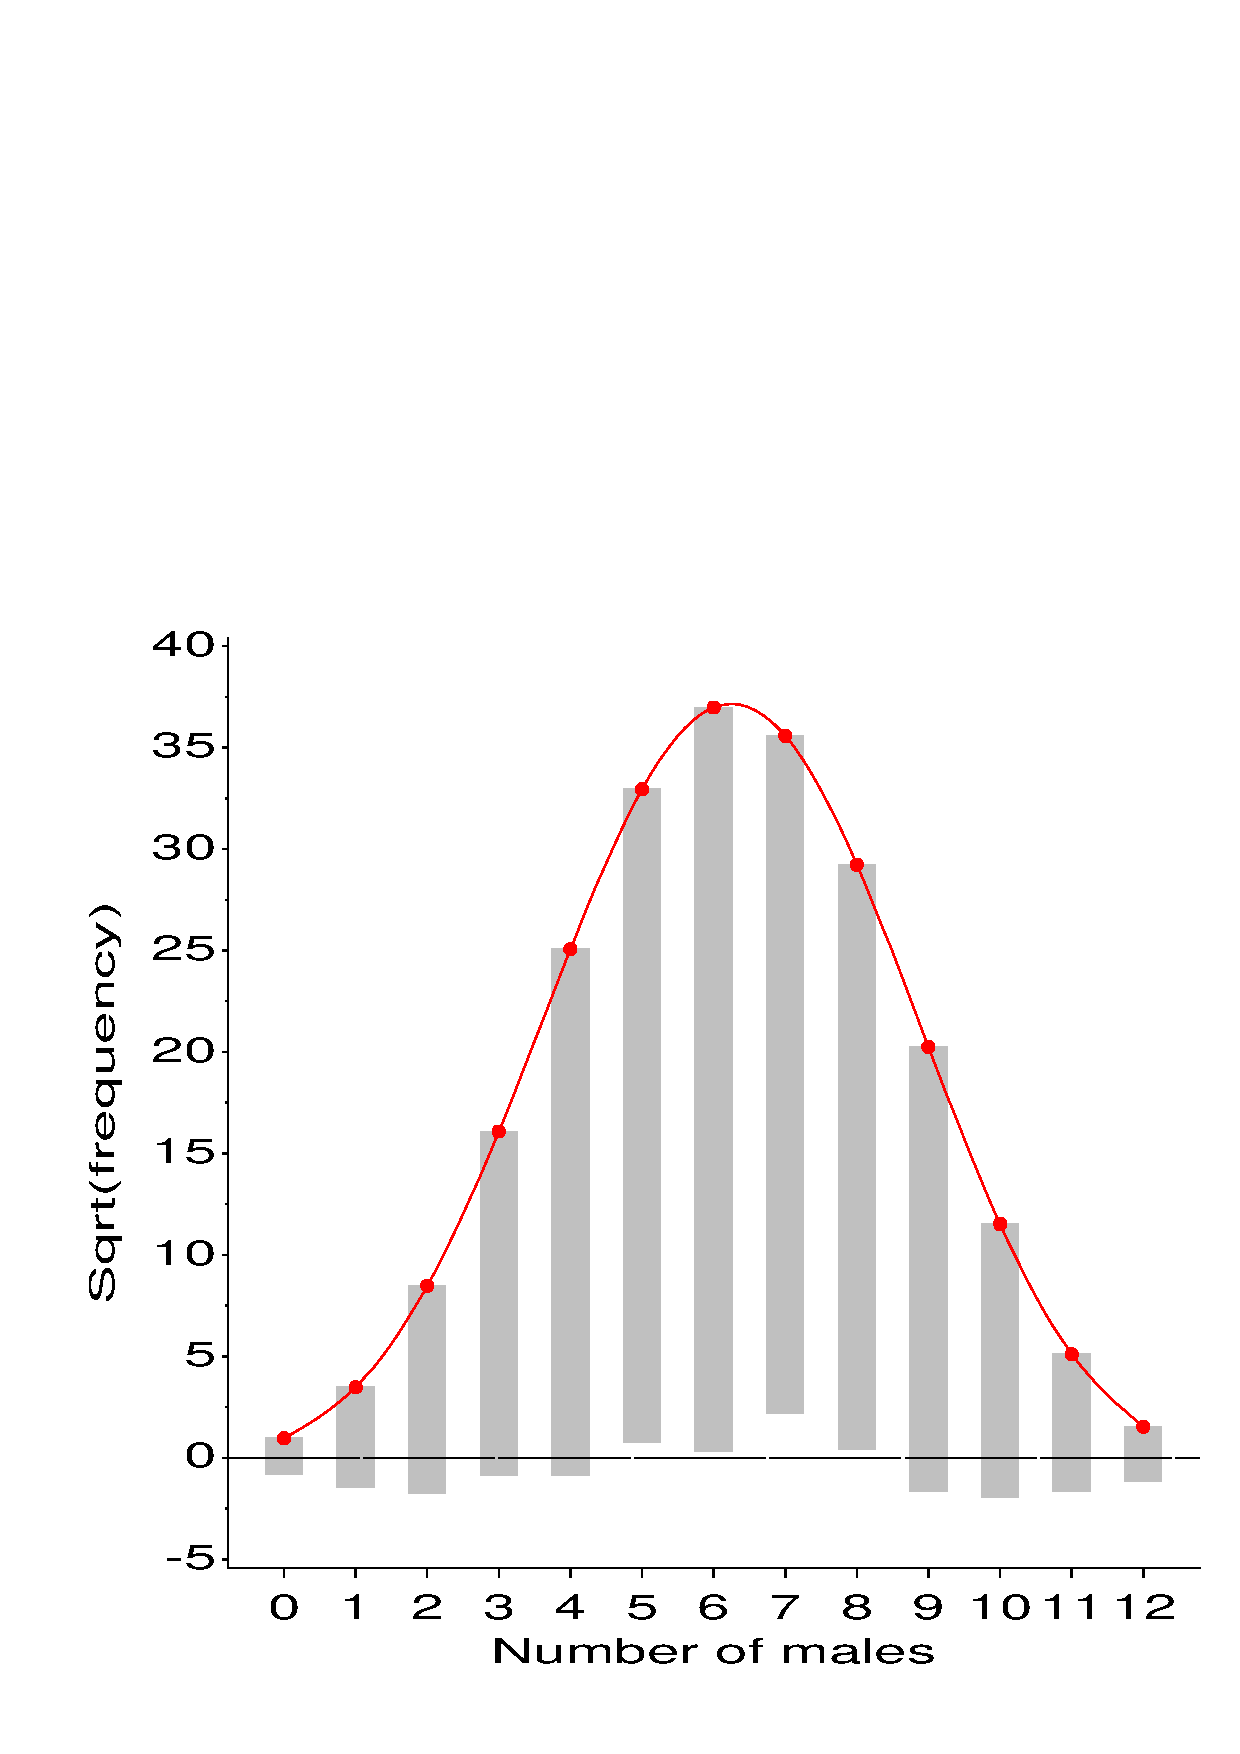
\includegraphics[width=1\linewidth]{saxony}\graphicsfile{ch2/fig/saxony.eps}{}
 \end{minipage}%
 \hfill
 \begin{minipage}[c]{.33\linewidth}
  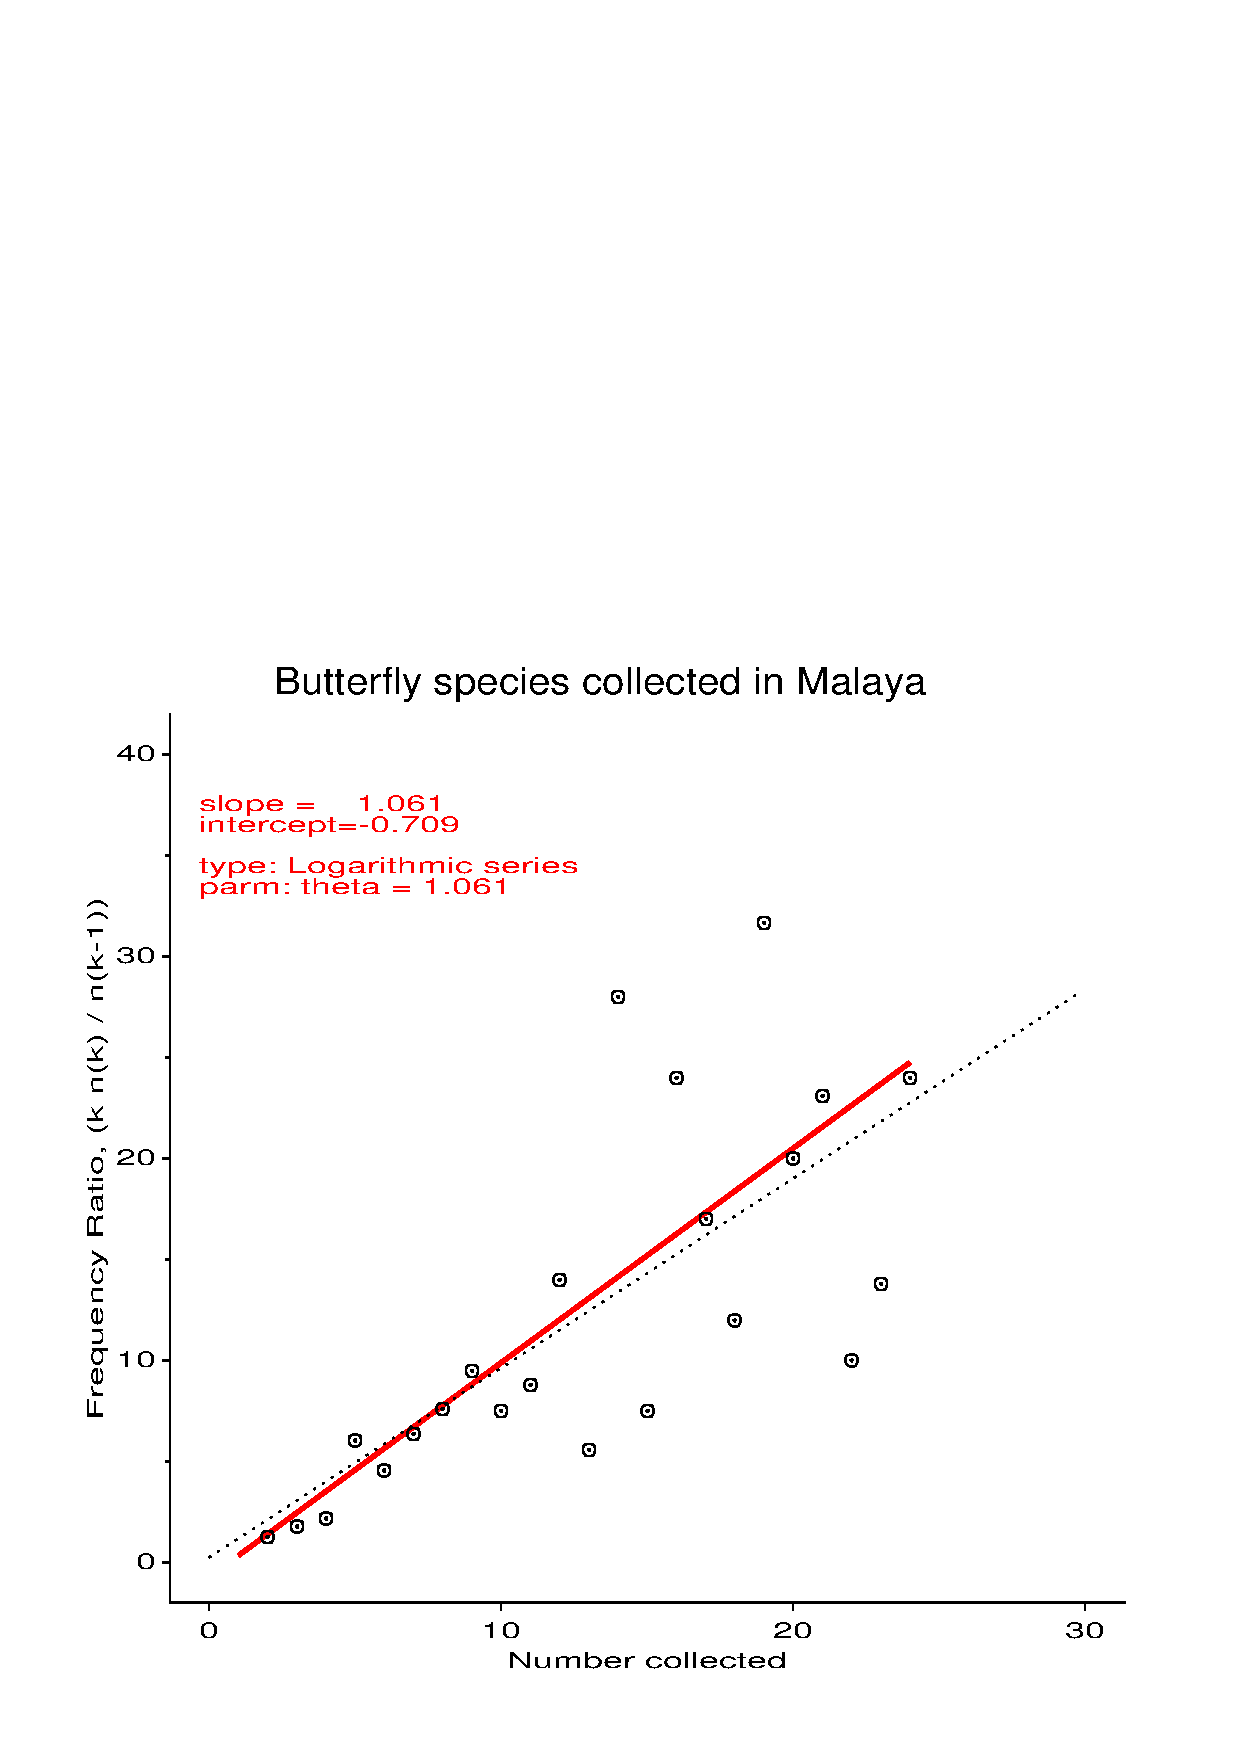
\includegraphics[width=1\linewidth]{orddemo3}\graphicsfile{ch2/fig/orddemo3.eps}{}
 \end{minipage}
 \hfill
 \begin{minipage}[c]{.33\linewidth}
  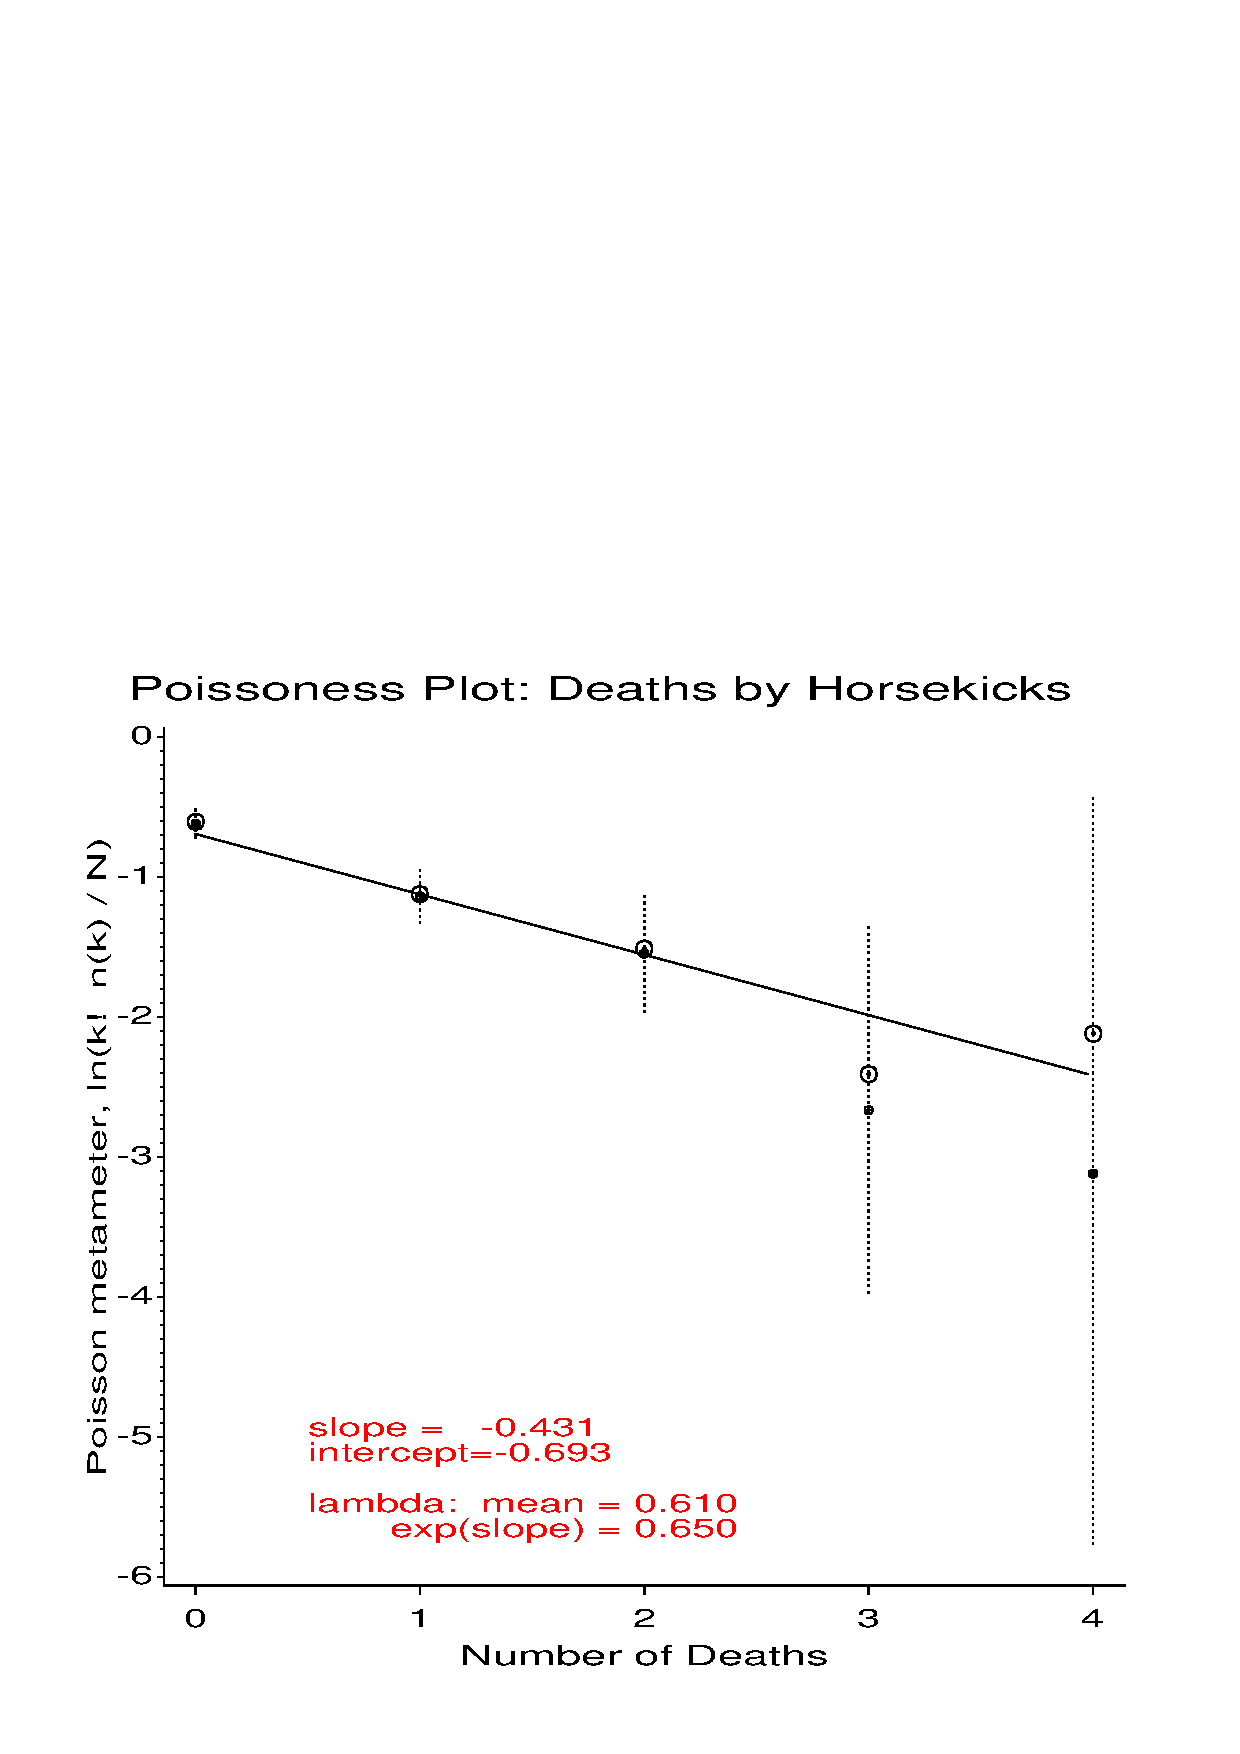
\includegraphics[width=1\linewidth]{poisdemo1}\graphicsfile{ch2/fig/poisdemo1.eps}{}
 \end{minipage}
\end{center}


\begin{quote}
{\Large\noindent
The analysis of two-way frequency tables concerns the association
between two variables.  Different specialized displays are focused
on visualizing an odds ratio ($2 \times 2$ tables), or the general
pattern of association, or the agreement between row and column
categories.}
\end{quote}
\minitoc
\clearpage

\section{Introduction}
\epigraph{If you choose to represent the various parts in life by
holes upon a table, of different shapes---some circular, some
triangular, some square, some oblong---we shall generally find that
the triangular person has got into the square hole, the oblong into
the triangular, and a square person has squeezed himself into the
round hole.}{Sydney Smith, 1769-1845}

Most methods of statistical analysis are concerned with understanding
relationships among variables.
With categorical variables, these relationships are usually
studied from data which has been
summarized by a
\glossterm{contingency table},
giving the frequencies of observations cross-classified
by two or more such variables.

This chapter is concerned with methods for understanding the association
between two categorical variables.
Some simple examples are also presented which involve a third, stratifying variable,
where we wish to determine if the relationship between two primary
variables is the same or different for all levels of the
stratifying variable.
Methods for fitting models and displaying associations for three-way
and larger tables are described in \chref{ch:mosaic}.

We describe briefly some methods for testing whether an association
exists between two variables and for quantifying the strength
of this association (\secref{sec:twoway-tests}).
In \secref{sec:twoway-strat} we extend these ideas to situations where
the relation between two variables is of primary interest, but there
are one or more background variables to be controlled.

The main emphasis, however, is on graphical methods which help
to describe the nature of an association between variables.
\secref{sec:twoway-fourfold} presents the fourfold display,
designed to portray the odds ratio in $2 \times 2$ tables or a set
of $k$ such tables.
Sieve diagrams (\secref{sec:twoway-sieve}) and association plots
(\secref{sec:twoway-assoc}) are more general methods for depicting
the pattern of associations an any two-way tables.
When the row and column variables represent the classifications
of different raters, specialized measures and visual displays
for inter-rater agreement (\secref{sec:twoway-agree}) are particularly
useful.
Another specialized display, the trilinear plot (\secref{sec:twoway-trilinear})
is designed
for three-column frequency tables or compositional data.
In order to make clear some of the distinctions which occur in
\ctab{} analysis, I begin with several examples.

\begin{Example}[berkeley1]{Berkeley admissions}
\tabref{tab:berk22} shows aggregate data on applicants to
graduate school at Berkeley for the six largest departments in 1973
classified by admission and gender
\citep{Bickel-etal:75}.
See \datref{dat:berkeley} for the complete data set.
For such data we might wish to study whether there is an association
between admission and gender.
Are male (or female) applicants more likely to be admitted?
The presence of an association might be considered as
evidence of sex bias in admission practices.

\tabref{tab:berk22} is an example of the simplest kind of \ctab,
a $2 \times 2$ classification of individuals according to two
dichotomous (binary) variables.
For such a table, the question of whether there is an association
between admission and gender is equivalent to asking if the
proportions of males and females who are admitted to graduate
school are the same, or whether the difference in proportions
admitted is zero.
\begin{table}[htb]
\caption{Admissions to Berkeley graduate programs}
\label{tab:berk22}
 \begin{center}
\begin{tabular}{lrr|rrr}
\hline
  & Admitted & Rejected & Total & \red{\% Admit} & \red{Odds(Admit)}\\
\hline
 Males & 1198 & 1493 & 2691  & \red{44.52} & \red{0.802}\\
 Females & 557 & 1278 & 1835 & \red{30.35} & \red{0.437}\\
\hline
 Total & 1755 & 2771 & 4526  & 38.78 & 0.633\\
\hline
\end{tabular}
\end{center}
\end{table}

\end{Example}

Although the methods for quantifying association in larger tables can be
used for $2 \times 2$ tables, there are specialized measures
(described in \secref{sec:twoway-tests}) and
graphical methods for these simpler tables.

It is frequently useful to make a distinction between \glossterm{outcome},
or response variables, on the one hand, and possible \glossterm{explanatory}
or predictor variables on the other.
In \tabref{tab:berk22}, it is natural to consider admission
as the outcome, and gender as the explanatory variable.
In other tables, no variable may be clearly identified as \emph{the}
outcome, or there may be several response variables.

\begin{Example}[haireye1]{Hair color and eye color}
\tabref{tab:hairdat} shows data collected by
\citet{Snee:74}
on the relation between hair color and eye color among 592
students in a statistics course
(\datref{dat:haireye}).  Neither hair color nor eye color
is considered a response in relation to the other;  our interest concerns
whether an association exists between them.
Hair color and eye color have both been classified
into four categories.  Although the categories used are among the most
common, they are not the only categories possible.%
\footnote{If students had been asked to write down their hair and eye
colors, it is likely that many more than four categories of each
would appear in a sample of nearly 600.}
Everyday observation suggests that there probably is an association
between hair color and eye color, and we will describe tests
and measures of associations for larger tables in
\secref{sec:twoway-overall}.
\begin{table}[htb]

\caption{Hair-color eye-color data}\label{tab:hairdat}
\begin{center}
\begin{tabular}{|lrrrr|r|}
\hline
        & \multicolumn{4}{c|}{Hair Color}        & \\
Eye     &         &         &         &         &       \\
Color   &  Black  &  Brown  &    Red  &  Blond  & Total \\[2ex] \hline
Green   &      5  &     29  &     14  &     16  &    64 \\
Hazel   &     15  &     54  &     14  &     10  &    93 \\
Blue    &     20  &     84  &     17  &     94  &   215 \\
Brown   &     68  &    119  &     26  &      7  &   220 \\[1ex] \hline
Total   &    108  &    286  &     71  &    127  &   592 \\ \hline
\end{tabular}
\end{center}
\end{table}


\end{Example}

Table variables may be treated simply as unordered,
\glossterm{nominal} variables,  or as
\glossterm{ordinal} variables, where the categories are
ordered according to some underlying dimension.
For example, the categories of hair color or eye color
are typically considered as nominal categories;
however, they
might arguably be considered to be ordered from light to dark.
When the variables are ordinal, more sensitive
and therefore more powerful tests of association can be used.

If, as we suspect, hair color and eye color are associated,
we would like to understand \emph{how} they are associated.
The graphical methods described later in this chapter help
reveal the pattern of associations present.

\begin{Example}[arthrit1]{Arthritis treatment}
The data in \tabref{tab:arthrit} compares an active treatment for rheumatoid
arthritis to a placebo
\citep{KochEdwards:88}.
The outcome reflects
whether individuals showed no improvement, some improvement, or
marked improvement.
Here, the outcome variable is an ordinal one, and it is probably
important to determine if the relation between treatment and outcome
is the same for males and females.
The data set is given more fully in \datref{dat:arthrit}.

This is, of course, a three-way table, with factors
Treatment, Sex, and Improvement.
If the relation between treatment and outcome is the same for
both genders, an analysis of the Treatment by Improvement
table (collapsed over sex) could be carried out.
Otherwise we could perform separate analyses for
men and women, or
treat the combinations of treatment and sex as four levels of
a ``population'' variable, giving a $4 \times 3$ two-way table.
These simplified approaches each ignore certain information
available in
an analysis of the full three-way table.
\begin{table}[tb]

\caption{Arthritis treatment data}\label{tab:arthrit}
\begin{center}
\begin{tabular}{ll|rrr|r}
\hline
     &  & \multicolumn{3}{c|}{Improvement}            &  \\
\hline
   Treatment&  Sex    &None    &Some    &Marked  &  Total \\[2ex]
\hline
   Active   &  Female &      6 &      5 &     16 &     27 \\
            &  Male   &      7 &      2 &      5 &     14 \\
\hline
   Placebo  &  Female &     19 &      7 &      6 &     32 \\
            &  Male   &     10 &      0 &      1 &     11 \\[1ex]
\hline
   Total    &         &     42 &     14 &     28 &     84 \\
\hline
\end{tabular}
\end{center}
\end{table}


\end{Example}

\section{Tests of association for two-way tables}\label{sec:twoway-tests}

\subsection{Notation and terminology}\label{sec:twoway-notation}
To establish notation, let \(\mat{N}  =  \{  n_{ij}  \}\) be the
observed frequency table of variables \(A\) and \(B\) with \(r\) rows
and \(c\) columns, as shown in \tabref{tab:rbyc}.
In what follows, a subscript is replaced by a ``$+$''
when summed over the corresponding variable, so \(n_{i+}  =  \sum_j \,
n_{ij}\) gives the total frequency in row \(i\), \(n_{+j}  =  \sum_i \,
n_{ij}\) gives the total frequency in column \(j\), and \(n_{++}  =
\sum_i \sum_j \,  n_{ij}\) is the grand total; for convenience,
\(n_{++}\) is also symbolized by \(n\).
\begin{table}[htb]
\caption[The R by C contingency table]{The $R \times C$ contingency table}
\label{tab:rbyc}
\vspace{1ex}
\begin{center}
\begin{tabular}{l|llll|l}
\hline
Row      & \multicolumn{4}{c|}{Column category}      &          \\
Category &   1      &   2      & $\cdots$  &  $C$    & Total    \\
\hline
   1     & $n_{11}$ & $n_{12}$ & $\cdots$ & $n_{1C}$ & $n_{1+}$ \\
   2     & $n_{21}$ & $n_{22}$ & $\cdots$ & $n_{2C}$ & $n_{2+}$ \\
$\vdots$ & $\vdots$ & $\vdots$ & $\cdots$ & $\vdots$ & $\vdots$ \\
   $R$   & $n_{R1}$ & $n_{R2}$ & $\cdots$ & $n_{RC}$ & $n_{R+}$   \\  
\hline
Total    & $n_{+1}$ & $n_{+2}$ & $\cdots$ & $n_{+C}$ & $n_{++}$   \\
\hline
\end{tabular}
\end{center}
\end{table}

When each observation is randomly sampled from some population
and classified on two categorical variables, $A$ and $B$,
we refer to the \glossterm{joint distribution} of these variables,
and let $\pi_{ij} = \Pr(A=i,\,B=j)$ denote the probability that
an observation is classified in row $i$, column $j$ (or cell $(ij)$)
in the table.
Corresponding to these population joint probabilities, the
cell proportions, $p_{ij} = n_{ij} / n$, give the sample joint
distribution.

The row totals $n_{i+}$ and column totals $n_{+j}$ are called marginal frequencies for variables $A$ and $B$ respectively.
These describe the distribution of each variable \emph{ignoring} the other.
For the population probabilities, the \glossterm{marginal distributions}
are defined analogously as the row and column totals of the 
joint probabilities,
$\pi_{i+} = \sum_j \pi_{ij}$, and
$\pi_{+j} = \sum_i \pi_{ij}$.
The sample marginal proportions are, correspondingly, 
$p_{i+} = \sum_j p_{ij} = n_{i+} / n$, and 
$p_{+j} = \sum_i p_{ij} = n_{+j} / n$.

When one variable (the column variable, $B$, for example) is a response
variable, and the other ($A$) is an explanatory variable,
it is most often useful to examine the distribution of the response $B$
for \emph{each} level of $A$ separately.
These define the \glossterm{conditional distributions} of $B$, given the
level of $A$, and are defined for the population as
$\pi_{j\given i} = \pi_{ij} / \pi_{i+}$.

These definitions are illustrated in \outref{out:berkfreq.1}.
For the Berkeley data (\tabref{tab:berk22}), it shows the joint frequencies, $n_{ij}$, and joint sample percentages,
$100 \times p_{ij}$, in the first two rows within each table cell.
The third row in each cell (``Row pct'')
gives the conditional percentage of admission or rejection,
$100 \times p_{j\given i}$ for males and females separately.
The row and column labelled ``Total'' give the
marginal frequencies, $n_{i+}$ and $n_{+j}$,
and marginal percentages, $p_{i+}$ and $p_{+j}$.

\begin{Output}[htb]
\caption{Admission to Berkeley graduate programs: joint, marginal, and conditional percents}\label{out:berkfreq.1}
\small
\verbatiminput{ch\thechapter/out/berkfreq.1}
\end{Output}

\renewcommand{\FileName}{twobytwo}

\begin{frame}
%\makeatletter\slidebox@restore\makeatother
\frametitle{Graphical Methods for 2$\times$2 tables: Example}
\begin{itemize}
 \item \citet{Bickel-etal:75}: data on admissions to graduate departments
 at Berkeley in 1973.
 \item Aggregate data for the six largest departments:
 \begin{table}[htb]
\caption{Admissions to Berkeley graduate programs}
\label{tab:berk22}
 \begin{center}
\begin{tabular}{lrr|rrr}
\hline
  & Admitted & Rejected & Total & \red{\% Admit} & \red{Odds(Admit)}\\
\hline
 Males & 1198 & 1493 & 2691  & \red{44.52} & \red{0.802}\\
 Females & 557 & 1278 & 1835 & \red{30.35} & \red{0.437}\\
\hline
 Total & 1755 & 2771 & 4526  & 38.78 & 0.633\\
\hline
\end{tabular}
\end{center}
\end{table}


 \item Evidence for gender bias?
 \begin{itemize}

 \item Odds ratio, 
 $\theta = \frac{\mbox{Odds}(\mbox{Admit}\given\mbox{Male})}{\mbox{Odds}(\mbox{Admit}\given\mbox{Female})} = 
 \frac{1198 / 1493}{557 / 1276} = \frac{0.802}{0.437} = 
 1.84$
 \item $\rightarrow$ Males 84\% more likely to be admitted. 
 \item Chi-square tests: $G^2_{(1)} = 93.7$, $\chi^2_{(1)} = 92.2, \: p < 0.0001$
 \end{itemize}
\end{itemize}

\end{frame}
\begin{frame}[plain]
\begin{center}
\includegraphics[width=.7\textwidth]{fig/Admissions2}
\end{center}
\begin{itemize*}
 \item How to analyse these data?
 \item How to visualize \& interpret the results?
 \item Does it matter that we collapsed over Department?
\end{itemize*}


\end{frame}

\subsection{Standard analysis}
\begin{frame}[fragile]
% \makeatletter\slidebox@restore\makeatother
 \frametitle{Standard analysis: PROC FREQ}

% \vspace{2ex}
\begin{Input}
 proc freq data=berkeley;
   weight freq;
   tables gender*admit / chisq;
\end{Input}
 Output:
\begin{Output}[gobble=7,baselinestretch=.8]
               Statistics for Table of gender by admit

       Statistic                     DF       Value      Prob
       ------------------------------------------------------
       Chi-Square                     1     92.2053    <.0001
       Likelihood Ratio Chi-Square    1     93.4494    <.0001
       Continuity Adj. Chi-Square     1     91.6096    <.0001
       Mantel-Haenszel Chi-Square     1     92.1849    <.0001
       Phi Coefficient                       0.1427          
\end{Output}
 How to visualize and interpret?
\end{frame}

\subsection{Fourfold displays}
\begin{frame}
% \makeatletter\slidebox@restore\makeatother
 \frametitle{Fourfold displays for 2 $\times$ 2 tables}
 \begin{itemize*}
 \item \boldital{Quarter circles}: radius $\sim \sqrt{n_{ij}} \Rightarrow$
 \textbf{area} $\sim$ \textbf{frequency}
 \item \boldital{Independence}: Adjoining quadrants $\approx$ align
 \item \boldital{Odds ratio}: ratio of areas of diagonally opposite cells
 \item \boldital{Confidence rings}: Visual test of 
 $H_0 : \theta = 1 \leftrightarrow$ \alert{adjoining rings overlap}

 \begin{center}
   \includegraphics[width=.45\dispwidth,clip]{fig/pie2x2g}
 \end{center}
 \item Confidence rings do not overlap: $\theta \neq 1$  (reject $H_0$)
 \end{itemize*}
\end{frame}

\begin{frame}
 %\makeatletter\slidebox@restore\makeatother
 \frametitle{Fourfold displays for 2 $\times$ 2 $\times $ \textit{k} tables}
 \begin{itemize*}
 \item Data in \tabref{tab:berk22} had been pooled over departments
 \item Stratified analysis: one fourfold display for each department
 \item Each $2 \times 2$ table standardized to equate marginal frequencies
 \item Shading: highlight departments for which $H_a : \theta_i \ne 1$

 \begin{center}
 %  \includegraphics[width=.6\dispwidth,clip]{fig/pie2x2bb.eps}
   \includegraphics[width=.6\dispwidth,clip]{fig/pie2x2b}
 \end{center}
 \item Only one department (A) shows association; $\theta_A = 0.349 \rightarrow
 $ women $(0.349)^{-1} = 2.86$ times as likely as men to be admitted.
 \end{itemize*}
 \end{frame}

\begin{frame}
 %\makeatletter\slidebox@restore\makeatother
   \frametitle{What happened here?}
  Why do the results \emph{collapsed over} department disagree with the results \emph{by} department?
  \begin{block}{Simpson's paradox}
   \begin{itemize}
	 \item<1-> Aggregate data are misleading because they falsely
	 assume men and women apply \emph{equally} in each field.
	 \item<2-> But:
	   \begin{itemize*}
	   \item Large differences in admission rates across departments.
	   \item Men and women apply to these departments differentially.
	   \item Women applied in large numbers to departments with low admission rates.
	 \end{itemize*}
	 \item<3->
	  Other graphical methods can show these effects.
 	 \item<3-> (This ignores possibility of \emph{structural bias} against women:
	 differential funding of fields to which women are more likely to apply.)
  \end{itemize}
  \end{block}
\end{frame}

\begin{frame}[fragile]
%\makeatletter\slidebox@restore\makeatother

\frametitle{The \sasprogt{FOURFOLD} and the \macrot{FFOLD}}
  \begin{itemize*}
  \item The \sasprog{FOURFOLD} is written in \IML.
  \item The \macro{FFOLD} provides a simpler interface.
  \item Printed output: (a) significance tests for individual odds ratios,
  (b) tests of homogeneity of association (here, over departments) and
  (c) conditional association (controlling for department).
  \end{itemize*}
Plot by department:
\begin{Input}[fontsize=\small,label=\fbox{\texttt{berk4f.sas}},baselinestretch=0.8]
%include catdata(berkeley);

%ffold(data=berkeley, 
   var=Admit Gender,       \sascomment{/* panel variables   */} 
   \sasemph{by=Dept},                \sascomment{/* stratify by dept  */}
   down=2, across=3,       \sascomment{/* panel arrangement */}
   htext=2);               \sascomment{/* font size         */}
\end{Input}
Aggregate data: first sum over departments,
using the \macro{TABLE}:
\begin{Input}[fontsize=\small,baselinestretch=0.9,firstnumber=8]
%table(data=berkeley, \sasemph{out=berk2}, 
   var=Admit Gender,       \sascomment{/* omit dept          */}
   weight=count,           \sascomment{/* frequency variable */}
   order=data);
%ffold(\sasemph{data=berk2}, var=Admit Gender);
\end{Input}
\end{frame}

\subsection{Odds ratio plots}
\begin{frame}[fragile]
\frametitle{Odds ratio plots}
\begin{Rin}
> library(vcd)
> oddsratio(UCBAdmissions, log=FALSE)
\end{Rin}
\begin{Rout}
    A     B     C     D     E     F 
0.349 0.803 1.133 0.921 1.222 0.828 
\end{Rout}
\begin{Rin}
> lor <- oddsratio(UCBAdmissions)  # capture log odds ratios
> plot(lor)
\end{Rin}
\begin{center}
   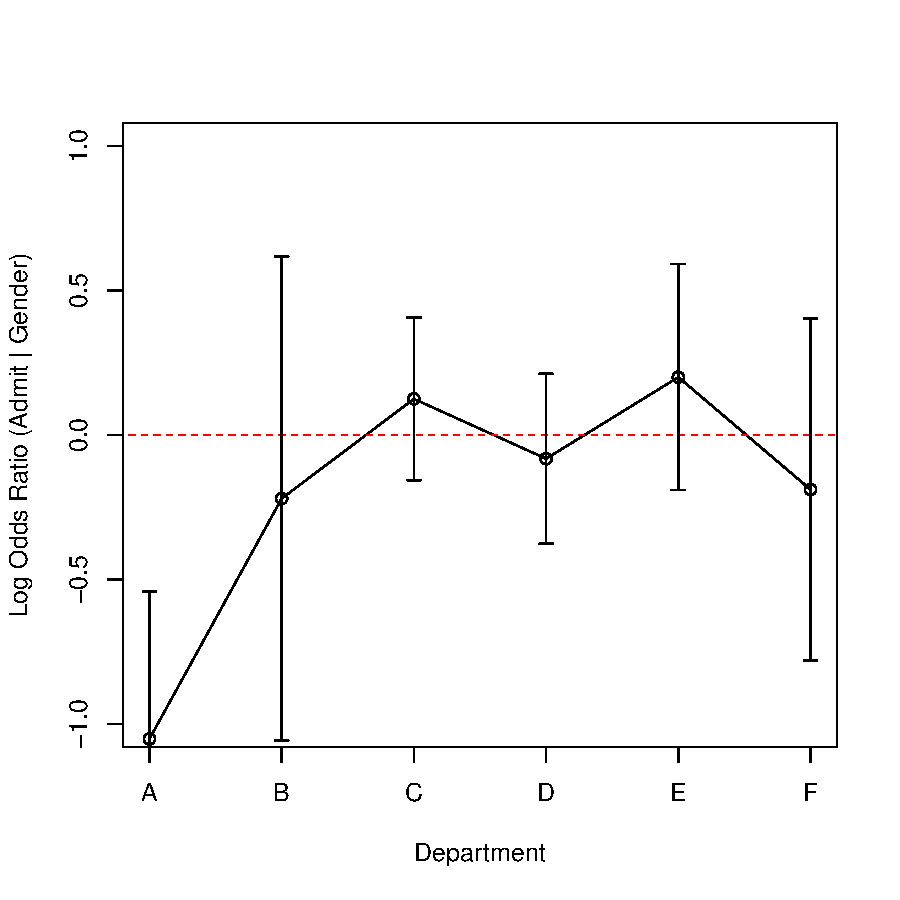
\includegraphics[width=.45\dispwidth,clip,trim=0 20 20 40]{fig/vcd-tut-oddsratio}
\end{center}

\end{frame}


\subsection{Larger tables---Overall analysis}\label{sec:twoway-overall}
For two-way tables overall tests of association can be carried out
using \PROC{FREQ}.
If the table has more than two factors (as in the
Arthritis Treatment data), the other factors will be
ignored (and collapsed) if not included the
\texttt{TABLES} statement.
This simplified analysis may be misleading if
the excluded factors interact with the factors used in the
analysis.

\begin{Example}[arthrit2]{Arthritis treatment}
Since the main interest is in the relation between treatment and
outcome, an overall analysis (which ignores sex) could be carried out
using \PROC{FREQ} as shown below.
\ixd{arthritis treatment}

\begin{listing}
title 'Arthritis Treatment: PROC FREQ Analysis';
data arth;
   input sex$ treat$ @;
   do improve = 'None  ', 'Some', 'Marked';
      input count @;
      output;
      end;
datalines;
Female  Active    6  5  16
Female  Placebo  19  7   6
Male    Active    7  2   5
Male    Placebo  10  0   1
;
*-- Ignoring sex;
proc freq order=data;
   weight count;
   tables treat * improve / cmh chisq nocol nopercent;
   run;
\end{listing}

In this analysis, note that:
\begin{itemize}
\item TREAT and IMPROVE are both character variables, which \PROC{FREQ}
       orders alphabetically (i.e., `Marked', `None', `Some') by
       default.  Because I want to treat the IMPROVE variable as
       ordinal, I used \texttt{order=data} on the \PROC{FREQ}
       statement to have the levels of IMPROVE ordered by their order
       of appearance in the \Dset.

\ix{Cochran-Mantel-Haenszel tests|(}
\item The \opt{chisq}{FREQ} gives the usual \(\chi^2\) tests
       (Pearson, Fisher's, etc.).  The \opt{cmh}{FREQ} requests the
       \IX{Cochran-Mantel-Haenszel tests}, including specialized
		 tests for ordinal variables.
\end{itemize}
The output, shown in \outref{out:arthfreq.1}, begins with the frequency table, including row
percentages.  The row percentages show a clear effect of treatment:
for people given the Active treatment, 51\% showed Marked improvement,
while among those given the Placebo, 67\% showed no improvement.

The results for the \opt{chisq}{FREQ} are also shown in \outref{out:arthfreq.1}.  All tests
show a significant association between treatment and outcome.

\begin{Output}
\caption{Arthritis treatment data, overall analysis}\label{out:arthfreq.1}
\small
\verbatiminput{ch3/out/arthfreq.1}
\end{Output}
\end{Example}

\subsection{Tests for ordinal variables}\label{sec:ordinaltests}

For \(r \times  c\) tables, different tests are applicable depending
on whether either or both of the row and column variables are
ordinal.  Tests which take the ordinal nature of a variable into
account are provided by the \opt{cmh}{FREQ} on the
\stmt{tables}{FREQ}.
These tests are based on assigning numerical scores to
the table categories;  the default (table) scores treat the levels as
equally spaced.  They generally have higher power when the pattern of
association is determined by the order of an ordinal variable.

For the arthritis data, these tests (\opt{cmh}{FREQ}) give the
output shown in \outref{out:arthfreq.2}.

\begin{Output}
\caption{Arthritis treatment data, overall analysis}\label{out:arthfreq.2}
\small
\verbatiminput{ch3/out/arthfreq.2}
\end{Output}

The three types of tests differ in the types of departure from
independence they are sensitive to:

\begin{itemize}
\item \boldital{General Association}.  When the row and column
       variables are both nominal (unordered) the only alternative
       hypothesis of interest is that there is \emph{some} association
       between the row and column variables.  The CMH test statistic
       is similar to the (Pearson) Chi-Square and Likelihood Ratio
       Chi-Square in the Statistics table; all have \((r - 1) (c -
       1)\) df.
\ix{Cochran-Mantel-Haenszel tests!general association}
\ix{likelihood ratio test}

\item \boldital{Row Mean Scores Differ}.  If the column variable is
       ordinal, assigning scores to the column variable produces a
       mean for each row.  The association between row and column
       variables can be expressed as a test of whether these means
       differ over the rows of the table, with \(r - 1\) df.  This
       is analogous to the Kruskal-Wallis non-parametric test (ANOVA
       based on rank scores).
\ix{Kruskal-Wallis test}
\ix{Cochran-Mantel-Haenszel tests!row means differ}

\item \boldital{Nonzero Correlation (Linear association)}.  When {\bf both} row and
       column variables are ordinal, we could assign scores to both
       variables and compute the correlation ($r$).  The Mantel-Haenszel
       \(\chi^2\) is equal to \(( N - 1) r^2\), where N is the total
       sample size.  The test is most sensitive to a pattern where
       the row mean score changes linearly over the rows.
\end{itemize}
\ix{Cochran-Mantel-Haenszel tests!linear association}
{\bf Notes}:

\begin{itemize}
\item Different kinds of scores can be assigned using the
\opt{scores}{FREQ}
on the \stmt{tables}{FREQ}, but only the
relative spacing of the scores is important.
The default, \pname{SCORES=TABLE} uses integer row and column numbers
for character variables, and numeric levels (or formatted equivalents)
for numeric variables.

\item When only one variable is ordinal, make it the {\bf last} one
       on the \stmt{tables}{FREQ}, because \PROC{FREQ} only computes
       means across the column variable.
\item When there are only $r=2$ rows (as there are here), the 
nonzero correlation and row
       means tests are equivalent.
		 In a $2 \times 2$ table, all three tests are identical.
\end{itemize}

\subsection{Sample CMH Profiles}\label{sec:Sample}

Two contrived examples may make the differences among these tests
more apparent.  Visualizations of the patterns of association
reinforces the aspects to which the tests are most sensitive.

\subsubsection{General Association}
\ix{Cochran-Mantel-Haenszel tests!general association|(}
The table below exhibits a
general association between variables $A$ and $B$, but no difference in
row means or linear association.  The row means are calculated by
assigning integer scores, $b_i = i$ to the column categories.
\figref{fig:cmhdemo}(a) shows
the pattern of association in this table graphically, as a sieve diagram
(described in \secref{sec:twoway-sieve}).

 \begin{center}
 \begin{tabular}{r|rrrrr|rr}
  \hline
   & b1 & b2 & b3 & b4 & b5 & Total & Mean \\ 
  \hline
  a1 & 0 & 15 & 25 & 15 & 0 & 55 & 3.0 \\ 
  a2 & 5 & 20 & 5 & 20 & 5 & 55 & 3.0 \\ 
  a3 & 20 & 5 & 5 & 5 & 20 & 55 & 3.0 \\ 
  \hline
  Total & 25 & 40 & 35 & 40 & 25 & 165 & 3.0\\ 
  Mean & 2.8 & 1.6 & 1.4 & 1.6 & 2.8 & 2.1\\
  \hline
 \end{tabular}
 \end{center}


This is reflected in the \PROC{FREQ} output shown in
\outref{out:cmhdemo.1}.
The chi-square values for non-zero correlation and different
row mean scores are exactly zero because the row means are all equal.
Only the general association test shows that $A$ and $B$
are associated.
\begin{Output}[ht]
\caption{General Association example: CMH tests}\label{out:cmhdemo.1}
\small
\verbatiminput{ch3/out/cmhdemo.1}
\end{Output}
\ix{Cochran-Mantel-Haenszel tests!general association|)}

\subsubsection{Linear Association}
\ix{Cochran-Mantel-Haenszel tests!linear association|(}
The table below contains a weak,
non-significant general association, but significant row mean
differences and linear associations.
The unstructured test of general association would therefore
lead to the conclusion that no association exists, while the
tests taking ordinal factors into account would conclude otherwise.
Note that the largest frequencies
shift towards lower levels of $B$ as the level of variable $A$ increases.
See \figref{fig:cmhdemo}(b) for a visual representation of this pattern.

 \begin{center}
 \begin{tabular}{r|rrrrr|rr}
  \hline
     & b1 & b2 & b3 & b4 & b5 & Total & Mean \\ 
  \hline
  a1 & 2 & 5 & 8 & 8 & 8 & 31 & 3.48 \\ 
  a2 & 2 & 8 & 8 & 8 & 5 & 31 & 3.19 \\ 
  a3 & 5 & 8 & 8 & 8 & 2 & 31 & 2.81 \\ 
  a4 & 8 & 8 & 8 & 5 & 2 & 31 & 2.52 \\ 
  \hline
  Total & 17 & 29 & 32 & 29 & 17 & 124 & 3.00 \\ 
  Mean & 3.1 & 2.7 & 2.5 & 2.3 & 1.9 & 2.5\\
  \hline
 \end{tabular}
 \end{center}


Note that the \(\chi^2\)-values for the row-means and non-zero
correlation tests in \outref{out:cmhdemo.2}
are very similar, but the correlation test is more
highly significant since it is based on just one degree of
freedom.

\begin{Output}[htb]
\caption{Linear Association example: CMH tests}\label{out:cmhdemo.2}
\small
\verbatiminput{ch3/out/cmhdemo.2}
\end{Output}

The differences in sensitivity and power among these tests is
analogous to the difference between general ANOVA tests and tests for
linear trend in experimental designs with quantitative factors:
The more specific test has greater power, but is sensitive to
a narrower range of departure from the null hypothesis.


%% two subfig side-by-side
\begin{figure}[htb]
 \begin{minipage}[b]{.49\linewidth}
  \includegraphics[width=1\linewidth]{ch3/fig/cmhdemo1}
 \end{minipage}%
 \hfill
 \begin{minipage}[b]{.49\linewidth}
  \includegraphics[width=1\linewidth]{ch3/fig/cmhdemo2}
 \end{minipage}
 \caption[Sieve diagrams for general association and linear association]{Sieve diagrams for two patterns of association. (a) General association (b) linear association.
 In each figure,
 cells with greater than expected frequency are shown with solid, blue cross hatching and the number of boxes is proportional to the observed frequency.}\label{fig:cmhdemo}
\end{figure}
\ix{Cochran-Mantel-Haenszel tests!linear association|)}
\ix{Cochran-Mantel-Haenszel tests|)}

\section{Stratified analysis}\label{sec:twoway-strat}
An overall analysis ignores other variables (like sex), by
collapsing over them.  It is possible that the treatment is effective
only for one gender, or even that the treatment has opposite effects
for men and women.
\ixd{arthritis treatment}

A stratified analysis:

\begin{itemize}

\item controls for the effects of one or more background variables.
       This is similar to the use of a blocking variable in an ANOVA
       design.

\item is obtained by including more than two variables in the {\tt
       tables} statement.  List the stratification variables {\bf
       first}.  To examine the association between TREAT and IMPROVE,
       controlling for both SEX and AGE (if available):

\begin{equation*}
   \mbox{\texttt{tables }}
   \overbrace{\rule{0in}{1.5ex}\mbox{\texttt{ age * sex }}}^{\mbox{\scriptsize stratify by}}
   \mbox{\texttt{ * }}
   \overbrace{\rule{0in}{1.5ex}\mbox{\texttt{ treat }}}^{\mbox{\scriptsize explanatory}}
   \mbox{\texttt{ * }}
   \overbrace{\rule{0in}{1.5ex}\mbox{\texttt{ improve;}}}^{\mbox{\scriptsize response}}
\end{equation*}

\end{itemize}

\begin{Example}[arthrit3]{Arthritis treatment}
The statements below request a stratified analysis of the arthritis
treatment data
with CMH tests,
controlling for sex.

{\small
\begin{verbatim}
*-- Stratified analysis, controlling for sex;
proc freq order=data;
   weight count;
   tables sex * treat * improve / cmh chisq nocol nopercent;
   run;
\end{verbatim}
}

\PROC{FREQ} gives a separate table for each level of the stratification
variables (\outref{out:arthfreq.3} and \outref{out:arthfreq.4}), plus overall (partial) tests controlling for the
stratification variables (\outref{out:arthfreq.5}).
\ixd{arthritis treatment}

\begin{Output}[htb]
\caption{Arthritis treatment data, stratified analysis}\label{out:arthfreq.3}
\small
\verbatiminput{ch3/out/arthfreq.3}
\end{Output}

Note that the strength of
association%
\glosstex{meas of assoc}
between treatment and outcome is quite
strong for females (\outref{out:arthfreq.3}).  In contrast, the results for males (\outref{out:arthfreq.4}) shows
a not-quite significant association, even by the 
more powerful Mantel-Haenszel test.
However,
note that there are too few males for the general association
\(\chi^2\) tests to be reliable (the statistic does not follow the
theoretical \(\chi^2\) distribution).
\begin{Output}[htb]
\caption{Arthritis treatment data, stratified analysis}\label{out:arthfreq.4}
\small
\verbatiminput{ch3/out/arthfreq.4}
\end{Output}

The individual tables are followed by the (overall) partial tests of
association controlling for sex, shown in \outref{out:arthfreq.5}.  Unlike the tests for each stratum,
these tests {\bf do not} require large sample size in the individual
strata -- just a large total sample size.  Note that the \(\chi^2\)
values here are slightly larger than those from the initial analysis
that ignored sex.
\ixd{arthritis treatment}

\begin{Output}[htb]
\caption{Arthritis treatment data, stratified analysis}\label{out:arthfreq.5}
\small
\verbatiminput{ch3/out/arthfreq.5}
\end{Output}
\end{Example}

\subsection{Assessing homogeneity of association}
In a stratified analysis
it is often of interest to know if the association between the
primary table variables is the same over all strata.  For \(k \times
2 \times  2\) tables this question reduces to whether the \IX{odds ratio} is
the same in all k strata, and \PROC{FREQ} computes the \IX{Breslow-Day test}
for homogeneity of odds ratios
when you use the \opt{measures}{FREQ} on the {\tt
tables} statement.  \PROC{FREQ} cannot perform tests of homogeneity for
larger tables, but these can be easily done with the \texttt{CATMOD}
procedure.
\ix{homogeneity of association}

\begin{Example}[arthrit4]{Arthritis treatment}
For the arthritis data, homogeneity means that there is no three-way
Sex * Treatment * Outcome association.  That is, the association
between treatment and outcome (\texttt{improve})
is the same for both men and women.
This hypothesis can be stated
as the \loglin\ model,
\begin{equation}\label{eq:STO2}
 \textrm{[SexTreat] [SexOutcome] [TreatOutcome]}
 \period
\end{equation}
This notation (described in \secref{sec:loglin-counts})
lists only the high-order association
terms in a linear model for log frequency.
Thus, the model \eqref{eq:STO2}
allows associations between sex and treatment (e.g., more males
get the Active treatment), between sex and outcome (e.g. females
are more likely to show marked improvement),
and between treatment and outcome,
but no three-way association.
In the \PROC{CATMOD} step
below, the \stmt{LOGLIN}{CATMOD} specifies this \loglin\  model
as \pname{sex|treat|improve@2} (where \texttt{improve} is the Outcome variable)
which means ``all terms up to 2-way
associations''.

\begin{listing}
title2 'Test homogeneity of treat*improve association';
data arth;
   set arth;
   if count=0 then count=1E-20;
proc catmod order=data;
   weight count;
   model sex * treat * improve = _response_ /
         ml noiter noresponse nodesign nogls ;
   loglin sex|treat|improve@2 / title='No 3-way association';
run;
   loglin sex treat|improve   / title='No Sex Associations';
\end{listing}
\ixd{arthritis treatment}

(Frequencies of zero can be regarded as either ``structural
zeros''---a cell which could not occur, or as ``sampling zeros''---a
cell which simply did not occur.  \PROC{CATMOD} treats zero frequencies
as ``structural zeros'', which means that cells with \texttt{count = 0}
are excluded from the analysis.  The DATA step above replaces the one
zero frequency by a small number.)
\ix{structural zeros}
\ix{sampling zeros}
\ix{zeros!structural}
\ix{zeros!sampling}

In the output from \PROC{CATMOD}
shown in \outref{out:arthfreq.7}, the likelihood ratio \(\chi^2\) (the
badness-of-fit for the No 3-Way model) is the test for homogeneity
across sex.  This is clearly non-significant, so the
treatment-outcome association can be considered to be the same for
men and women.

\begin{Output}[htb]
\caption{Arthritis treatment data, testing homogeneity}\label{out:arthfreq.7}
\small
\verbatiminput{ch3/out/arthfreq.7}
\end{Output}

Note that the associations of sex with treatment and sex with outcome
are both small and of borderline significance, which suggests a
stronger form of homogeneity, the log-linear model [Sex]
[TreatOutcome] which says the only association is that between
treatment and outcome.  This model is tested by the second {\tt
loglin} statement given above, which produced the results shown
in \outref{out:arthfreq.8}.
The likelihood ratio test indicates that this model might provide a
reasonable fit.
\ix{homogeneity of association}
\begin{Output}[htb]
\caption{Arthritis treatment data, testing homogeneity}\label{out:arthfreq.8}
\small
\verbatiminput{ch3/out/arthfreq.8}
\end{Output}
\end{Example}


\section{Fourfold display for 2 x 2 tables}\label{sec:twoway-fourfold}
\ixon{fourfold display}
The \boldital{fourfold display} is a relative of the pie chart,
designed for the display of $2 \times 2$ (or $2 \times 2 \times k$)
tables
\citep{Fienberg:75,Friendly:94b,Friendly:94c}.
In this display the frequency
\(n_{ij}\) in each cell of a fourfold table is shown by a quarter
circle, whose radius is proportional to \(\sqrt { n_{ij} }\), so the
area is proportional to the cell count.
The fourfold display
is similar to a pie chart in using segments of
a circle to show frequencies.  It
differs from a pie chart in that it keeps the
angles of the segments constant and varies the radius,
whereas the pie chart varies the angles and keeps the radius constant.

The main purpose of this display is to depict the sample odds ratio,
\(\hat{\theta} = (n_{11} /  n_{12} )
\div  (n_{21} /  n_{22} )\).  An association between the variables
(\(\theta \neq 1\)) is shown by the tendency of diagonally opposite
cells in one direction to differ in size from those in the opposite
direction, and the display uses color or shading to show this
direction.  Confidence rings for the observed \(\theta\) allow a
visual test of the hypothesis of independence,
 \(H_0 :  \theta  =  1\).  They have
the property that (in a standardized display) the rings for adjacent quadrants overlap \emph{iff}
the observed counts are consistent with the null hypothesis.

\begin{Example}[berkeley2]{Berkeley admissions}
\figref{fig:fourfold11} shows the basic fourfold display for the
Berkeley admissions data (\tabref{tab:berk22}).
Here, the area of each quadrant is proportional to the cell frequency,
shown numerically in each corner.
The odds ratio is proportional to the product of the areas
shaded dark, divided by the product of the areas shaded light.
The sample odds ratio, Odds (Admit\(|\)Male) / Odds(Admit\(|\)Female) is
1.84 (see \exref{ex:berkeley1a})
indicating that males were nearly twice as likely to be admitted.

However, it is difficult to make these visual comparisons
because there are more men than women, and because the
proportions admitted and rejected are unequal.  In the unstandardized
display the confidence bands have no interpretation as a test
of \(H_0 :  \theta  =  1\).
\fig{fourfold11}{scale=.6}{Fourfold display for Berkeley admission data, unstandardized}


The data in a $2 \times 2$ table can be standardized to make these
visual comparisons easier.
\tabref{tab:berkrow} shows the Berkeley data with the addition of
row percentages (which equate for the number of men and women applicants)
 indicating the proportion of each gender accepted
and rejected.
We see that 44.52\% of males were admitted, while only 30.35\% of
females were admitted.
Moreover, the row percentages have the same odds ratio as the
raw data: $44.52 \times 69.65 / 30.35 \times 55.48 = 1.84$.
\figref{fig:fourfold12} shows the fourfold display where
the area of each quarter circle is proportional to these row
percentages.

With this standardization, the confidence rings have the property
that the confidence rings for each upper quadrant will overlap
with those for the quadrant below it if the
odds ratio does not differ from 1.0.
No similar statement can be made about the
corresponding left and right quadrants, however, because
the overall rate of admission has not been standardized.
\begin{table}[htb]
\caption{Admissions to Berkeley graduate programs, Frequencies and Row Percentages}
\label{tab:berkrow}
 \begin{center}
\begin{tabular}{lrr|rr}
\hline
  & \multicolumn{2}{c|}{Frequencies} &\multicolumn{2}{c}{Row Percents} \\
  & Admitted & Rejected & Admitted & Rejected  \\
\hline
 Males  & 1198 & 1493 &  44.52 & 55.48  \\
 Females & 557 & 1278 &  30.35 & 69.65  \\
\hline
\end{tabular}
\end{center}
\end{table}
\fig{fourfold12}{scale=.6}{Fourfold display for Berkeley admission data, genders equated}


As a final step, we can standardize the data so that both table margins
are equal, while preserving the odds ratio.
Each quarter circle is then drawn to have an area
proportional to this standardized cell frequency.  This makes it
easier to see the association between admission and sex without being
influenced by the overall admission rate or the differential tendency
of males and females to apply.  With this standardization, the four
quadrants will align (overlap) horizontally and vertically
when the odds ratio is 1, regardless of the
marginal frequencies.  The fully standardized display, which is
usually the most useful form, is shown in \figref{fig:fourfold13}.

%\fig{fourfold13}{scale=.6}{Fourfold display for Berkeley admission data, genders and admission equated%
%. The area of each shaded
%quadrant shows the frequency, standardized to equate the margins for
%sex and admission.  Circular arcs show the limits of a 99\% confidence
%interval for the odds ratio.}
\begin{figure}[htb]
  \centering
  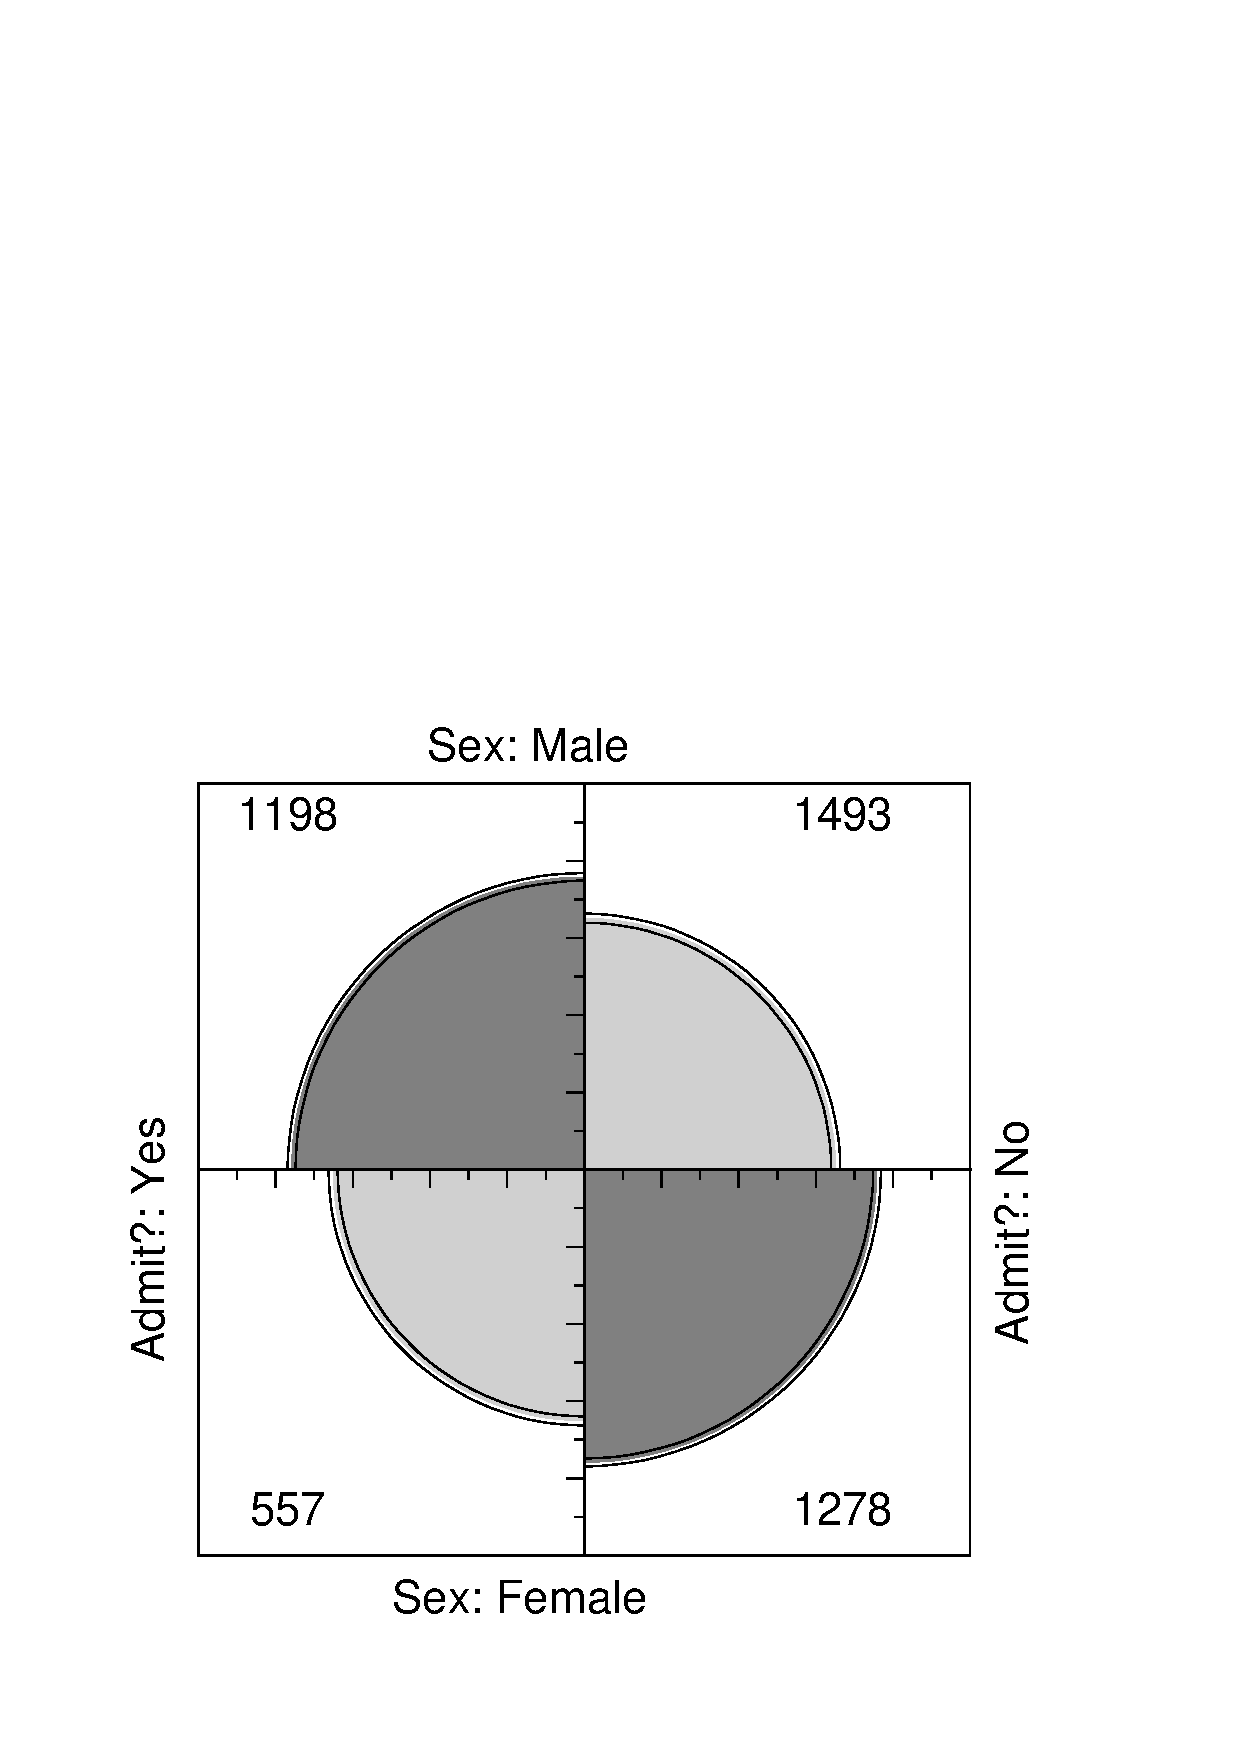
\includegraphics[scale=.6]{ch3/fig/fourfold13}
  \caption[Fourfold display for Berkeley admission data, genders and admission equated]{Fourfold display for Berkeley admission data, genders and admission equated%
. The area of each
quadrant shows the frequency, standardized to equate the margins for
sex and admission.  Circular arcs show the limits of a 99\% confidence
interval for the odds ratio.}\label{fig:fourfold13}
\end{figure}


The quadrants in \figref{fig:fourfold13} do not align and
the 99\% confidence rings around each quadrant do not overlap,
indicating that the odds ratio differs significantly from 1---putative
evidence of gender bias.  The very narrow
width of the confidence rings gives a visual indication of the
precision of the data---if we stopped here, we might feel quite confident of
this conclusion.
\end{Example}

\subsection{Confidence rings for odds ratio}
\ixon{fourfold dislplay!confidence rings}
Confidence rings for the fourfold display are computed from a
confidence interval for \(\theta\), whose endpoints can each be
mapped into a \(2 \times  2\) table.  Each such table is then drawn
in the same way as the data.

The interval for \(\theta\) is most easily found by considering the
distribution of \(\hat{\psi}  =  \log  \hat{\theta} \), whose standard
error may be estimated by \eqref{eq:aselogtheta}.  Then an approximate \(1  -  \alpha\) confidence
interval for \(\psi\) is given by
\begin{equation*}
 \hat{\psi} \,\pm\,  \hat{s} ( \hat{\psi} )  \:
z_{ 1 - \alpha  / 2 } =  \{ \hat{\psi}_l , \,  \hat{\psi}_u \} 
 \comma
\end{equation*}
as described in \secref{sec:twoway-twobytwo}.
The
corresponding limits for the odds ratio \(\theta\) are 
\(\{ \exp ( \hat{\psi}_l ) , \,  \exp ( \hat{\psi}_u ) \}\).  For the data
shown in \figref{fig:fourfold13}, 
\(\hat{\psi}  =  \log \,  \hat{\theta} =  .6104\), 
and \(\hat{s}  ( \hat{\psi} )  =  0.0639\), so the 99\%,
limits for \(\theta\) are \(\{ 1.5617, \,  2.1704 \}\).

Now consider how to find a \(2 \times  2\) table whose frequencies
correspond to the odds ratios at the limits of the confidence
interval.  A table standardized to equal row and column margins can
be represented by the \(2 \times  2\) matrix with entries
\begin{equation*}
 \left[
  \begin{array}{cc}
   p & (1-p) \\
  (1-p) & p
  \end{array}
 \right]
 \comma
\end{equation*}
whose odds ratio is \(\theta  =  p^2 /  ( 1  -  p)^2\).  
Solving for $p$ gives \(p  =  \sqrt \theta /  ( 1  +  \sqrt \theta )\).  The
corresponding frequencies can then be found by adjusting the
standardized table to have the same row and column margins as the
data. The results of these computations which generate the confidence
rings in \figref{fig:fourfold13} are shown in \tabref{tab:berkodds}.

\begin{table}[htb]
\caption{Odds ratios and equivalent tables for confidence rings.}\label{tab:berkodds}
 \begin{center}
\begin{tabular}{lr|rr|rr}
\hline
   &      Odds    & \multicolumn{2}{c|}{Standardized} & \multicolumn{2}{c}{Equivalent}  \\
   &      Ratio   & \multicolumn{2}{c|}{Table}   &  \multicolumn{2}{c}{Frequencies} \\
\hline
Lower &   1.562   &    0.555 & 0.445   &  1157.2 &  1533.8 \\
limit &           &    0.445 & 0.555   &   597.8 &  1237.2 \\[2ex]

Data  &   1.841   &    0.576 & 0.424   &  1198.0 &  1493.0 \\
      &           &    0.424 & 0.576   &   557.0 &  1278.0 \\[2ex]

Upper &   2.170   &    0.596 & 0.404   &  1237.8 &  1453.2 \\
limit &           &    0.404 & 0.596   &   517.2 &  1317.8 \\
\hline
\end{tabular}
\end{center}
\end{table}
\ixoff{fourfold dislplay!confidence rings}

\subsection{The \sasprog{FOURFOLD}}
Fourfold displays have been implemented in \IML{}.
The program is described in detail in an article in
\emph{Observations}
\citep{Friendly:94c}, and is listed and documented in
\macref{mac:fourfold}.

\texttt{fourfold} is a \IML{} module which is called as follows:
\begin{listing}
run fourfold(dim, table, vnames, lnames);
\end{listing}
where \texttt{table} is the $2 \times 2$ (or $2 \times 2 \times k$) frequency table whose dimensions are given by \texttt{dim};
\texttt{vnames} is a character vector containing the names of the table
variables, and
\texttt{lnames} is a character matrix of the category levels.
A variety of options for standardization, shading patterns and colors,
confidence rings, etc.\ are controlled by global variables,
described in \macref{mac:fourfold}.

To use the program, \texttt{\%include} the \sasprog{FOURFOLD}
within a \PROC{IML} step.  Then
enter the observed frequencies in an array \texttt{table},
and create a character vector \texttt{vnames} containing
the row and column variable names, and a two-row
character matrix \texttt{lnames} containing the
category labels.


For example, the plots in \figref{fig:fourfold11} and \figref{fig:fourfold13}
are produced by the statements below.
\begin{listing}
goptions hsize=7in vsize=7in;     *-- make plot square;

filename fourfold  \emph{'path/to/fourfold.sas'};
proc iml;
   %include fourfold;

   *-- Berkeley Admissions data;
   dim = \{2 2\};
   vnames = \{"Admit?" "Sex"\};
   lnames = \{"Yes" "No",
             "Male"  "Female"\};

          /* Admit Not */
   table = \{1198   1493,
             557   1278\};

   patterns=\{solid solid\};
   colors=\{grayd0 gray80\};

   std='MAX';               /* \figref{fig:fourfold11} */
   run fourfold(dim, table, vnames, lnames);

   std='MARG';              /* \figref{fig:fourfold13} */
   run fourfold(dim, table, vnames, lnames);
quit;
\end{listing}
The global variable \texttt{std} determines the way the table is
standardized.
\texttt{std='MAX'} scales the frequencies so that the largest value
is 100; \texttt{std='MARG'} is used to equate the marginal frequencies
for the row variable, the column variable, or both (the default).
The variable(s) equated are controlled by the global \texttt{config}
variable.  For example, to equate the second variable, as in \figref{fig:fourfold12},
you would specify \texttt{config=\{2\}}:
\begin{listing}
   std='MARG';
   config=\{2\};             /* \figref{fig:fourfold12} (equate gender) */
   run fourfold(dim, table, vnames, lnames);
\end{listing}

\subsection{Stratified analysis for $2 \times 2 \times k$ tables}\label{sec:twoway-fourstrat}
In a \(2 \times  2 \times  k\)
table, the last dimension often corresponds to ``strata'' or
populations, and it is typically of interest to see if the
association between the first two variables is homogeneous across
strata.  For such tables, simply make one fourfold panel for each
stratum.  The standardization of marginal frequencies is designed to
allow easy visual comparison of the pattern of association
when the marginal frequencies vary across two
or more populations

The admissions data shown in
\figref{fig:fourfold11}--\figref{fig:fourfold13} were actually obtained
from six departments ---the six largest at Berkeley
\citep{Bickel-etal:75}.
To determine the source of the apparent sex
bias in favor of males, we make a new plot, \figref{fig:pie2x2b},
stratified by department.
\ixd{Berkeley admissions}

Surprisingly, \figref{fig:pie2x2b} shows that, for five of the
six departments, the odds of admission is approximately the same for
both men and women applicants.  Department A appears to differs from
the others, with women approximately 2.86 (\(=  ( 313/19 )  /
(512/89)\)) times as likely to gain admission.  This appearance is
confirmed by the confidence rings, which in \figref{fig:pie2x2b}
are joint 99\% intervals for \(\theta_c ,  \,  c = 1, \dots ,
k\).

\begin{figure}[htb]
  \centering
  \includegraphics[scale=.8]{ch3/fig/pie2x2b}
  \caption[Fourfold display of Berkeley
admissions, by department]{Fourfold display of Berkeley
admissions, by department.  In each panel the confidence rings for
adjacent quadrants overlap if the odds ratio for admission and sex
does not differ significantly from 1.  The data in each panel have
been standardized as in \figref{fig:fourfold13}.}\label{fig:pie2x2b}
\end{figure}

This result, which contradicts the display for the aggregate data in
\figref{fig:fourfold13}, is a nice example of
\emph{Simpson's paradox}%
\footnote{Simpson's paradox \citep{Simpson:51} occurs in a three-way
table, $[A, B, C]$, when the marginal association between two variables,
$A, B$ collapsing over $C$ differs in \emph{direction} from the partial
association $A, B | C= c_k$ at the separate levels of $C$.
Strictly speaking, Simpson's paradox would require that for all
departments separately the odds ratio $\theta_k < 1$
(which occurs for Departments A, B, D, and F in \figref{fig:pie2x2b})
while in the aggregate data $\theta > 1$.
},
and illustrates clearly why an overall analysis of a three- (or higher-)
way table can be misleading.
\ix{Simpson's paradox}
The resolution of this contradiction can be found in the large
differences in admission rates among departments.  Men and women
apply to different departments differentially, and in these data
women happen to apply in larger numbers to departments that have a low
acceptance rate.  The aggregate results are misleading because they
falsely assume men and women are equally likely to apply in each
field.\footnote{This explanation ignores the possibility of structural bias
against women, e.g.,\ lack of resources allocated to departments that
attract women applicants.}

\begin{changebar}
Some final enhancements
of the fourfold display are
 shown in \figref{fig:pie2x2b2}.
Here (a) small tick marks are drawn to show the direction of association
(positive residuals)
and (b) the
\end{changebar} 
intensity of the shading colors is varied to distinguish
those strata for which the odds ratio differs significantly from 1
at $\alpha = .01$.%
\footnote{The \sasprog{FOURFOLD} allows these tests to be done either
individually or jointly (using a Bonferroni adjustment).}

\begin{figure}[htb]
  \centering
  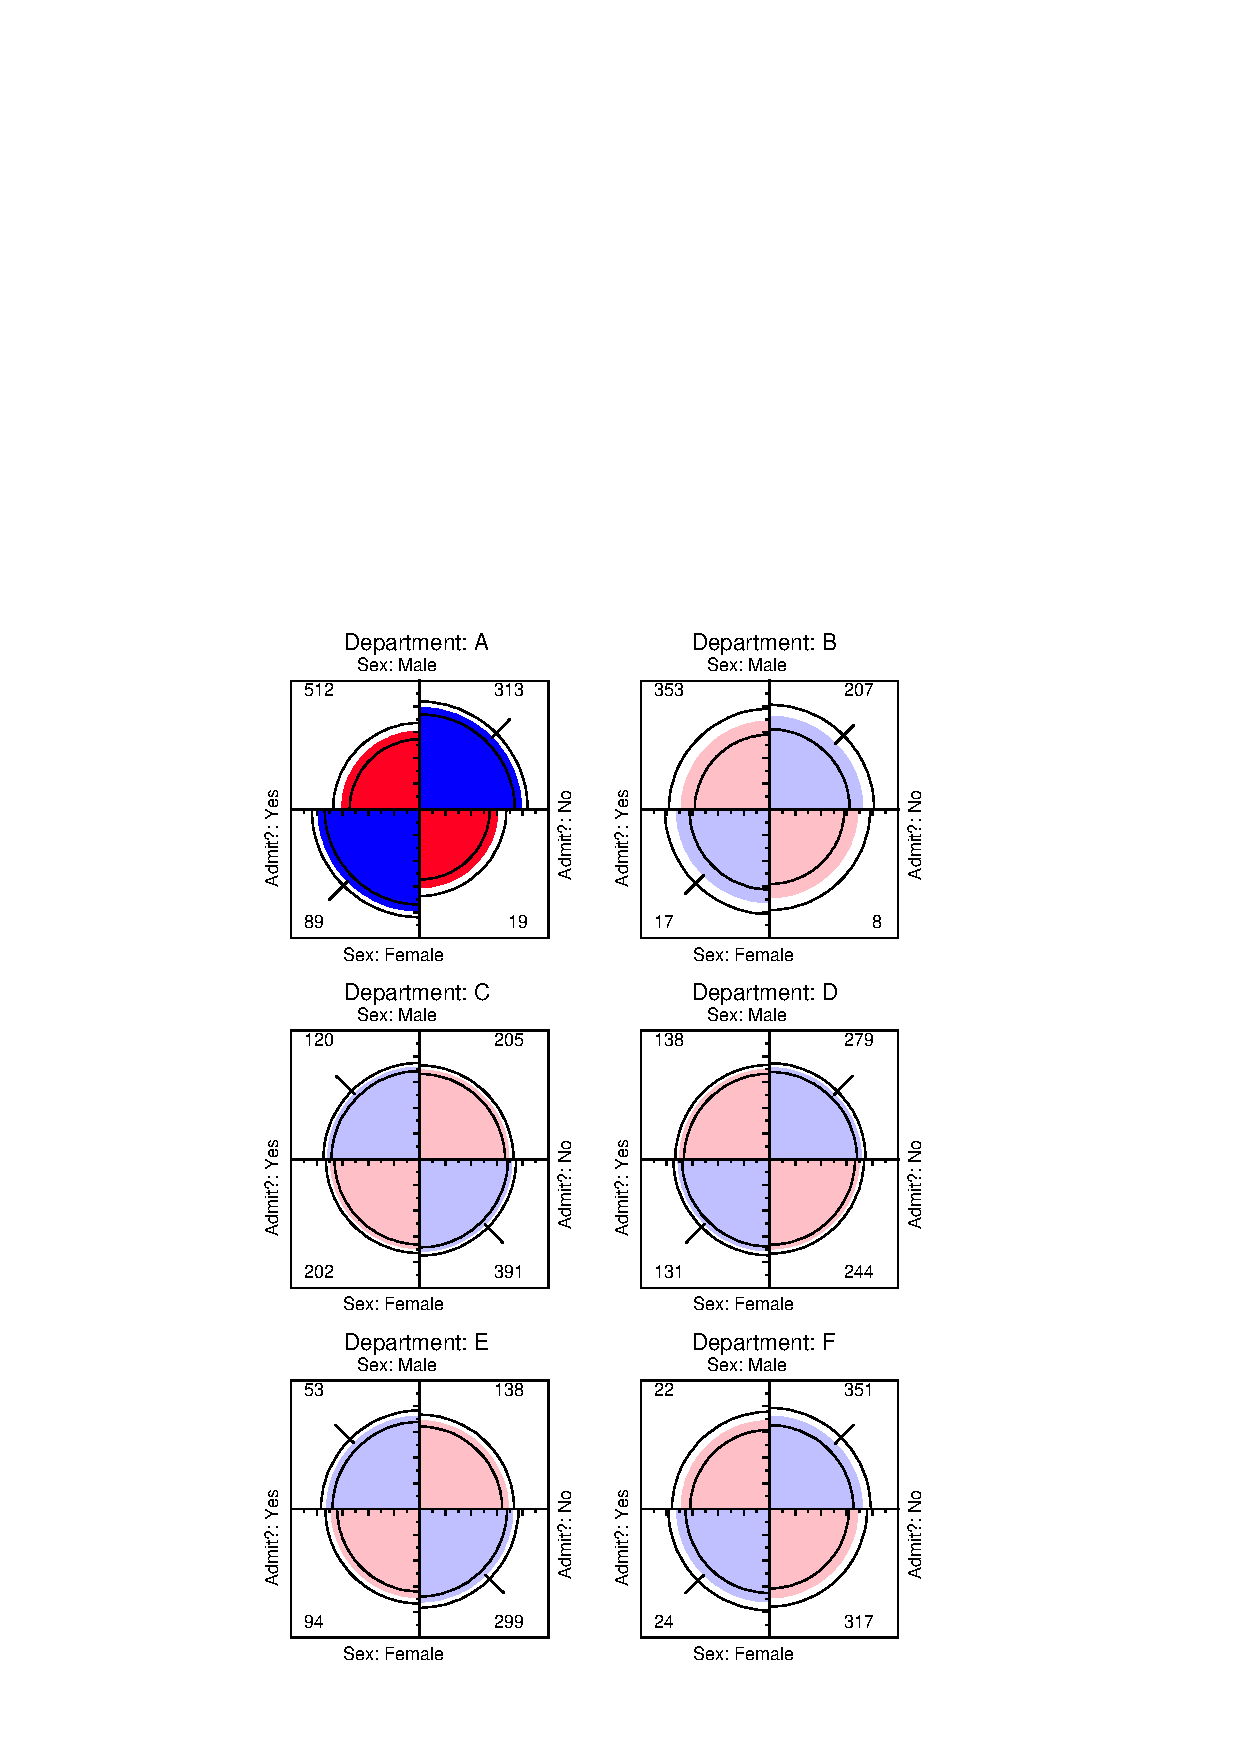
\includegraphics[scale=.8]{ch3/fig/pie2x2b2}
  \caption[Fourfold display of Berkeley
admissions, by department, enhanced]{Fourfold display of Berkeley
admissions, by department, enhanced.  Each panel is shaded
according to whether or not the odds ratio for admission and sex
differs significantly from 1.}\label{fig:pie2x2b2}
\end{figure}

\subsubsection{Visualization principles}
An important principle in the display of large, complex \Dsets\
is \boldital{controlled comparison}---we want to make comparisons
against a clear standard, with
other things held constant.
The fourfold display
differs from a pie chart in that it holds the
angles of the segments constant and varies the radius.
An important consequence is that we can quite easily compare a
series of fourfold displays for different strata, since corresponding
cells of the table are always in the same position.
As a result, an array of fourfold displays serve the goals of comparison and
detection better than an array of pie charts.
Moreover, it allows the observed frequencies to be standardized
by equating either the row or column totals, while preserving
the odds ratio.
In \figref{fig:pie2x2b}, for example,
the proportion of men and women, and the proportion
of accepted applicants were equated visually in each department.
This provides a clear standard which
also greatly facilitates controlled comparison.

Another principle is \boldital{visual impact}---we want the important
features
of the display to be easily distinguished from the less important
\citep{Tukey:93}.
\figref{fig:pie2x2b2} distinguishes the one department for which
the odds ratio differs significantly from 1 by shading intensity,
even though the same information can be found by inspection of the
confidence rings.

\begin{Example}[wheeze1]{Breathlessness and wheeze in coal miners}
The various ways of standardizing a collection of $2 \times 2$ tables
allows visualizing relations with different factors
(row percentages, column percentages, strata totals) controlled.
Different graphs can speak more eloquently to different questions.

\citet[Table 7.11]{Agresti:90} cites data from
\citet{AshfordSnowden:70} on the association between
two pulmonary conditions, breathlessness and wheeze, in a large sample of coal miners.
The miners are classified into age groups, and the question treated
by Agresti is whether the association between these two symptoms
is homogeneous over age.%
\footnote{A ninth group, aged 20-24 has been omitted from these
analyses.}
This question is addressed by displaying the odds ratio
in the $2 \times 2$ tables with the margins of breathlessness
and wheeze equated (i.e., with the default \pname{std='MARG';} option),
which gives the graph shown in \figref{fig:pie2x2wh1}.
Although the panels for all age groups show an overwhelmingly
positive association between these two symptoms, one can also
see that the strength of this association declines with increasing
age.

Note that the pattern of change over age is somewhat subtle
compared to the dominant positive association within each
panel.
When the goal is to display how the odds ratio varies with
a quantitative factor such as age, it is often better to simply
plot the odds ratio directly, as shown in \figref{fig:pie2x2wh2}.

The \sasprog{FOURFOLD} also provides the relevant test statistics,
shown in \outref{out:pie2x2wh}.
The test of whether the association is the same over age
is a test of the \loglin{} model
[BW][BA][WA] of no three-way association among the
variables Breathlessness, Wheeze and Age,
which is soundly rejected,
$G^2 (7) = 26.13$.

\begin{figure}[htb]
  \centering
  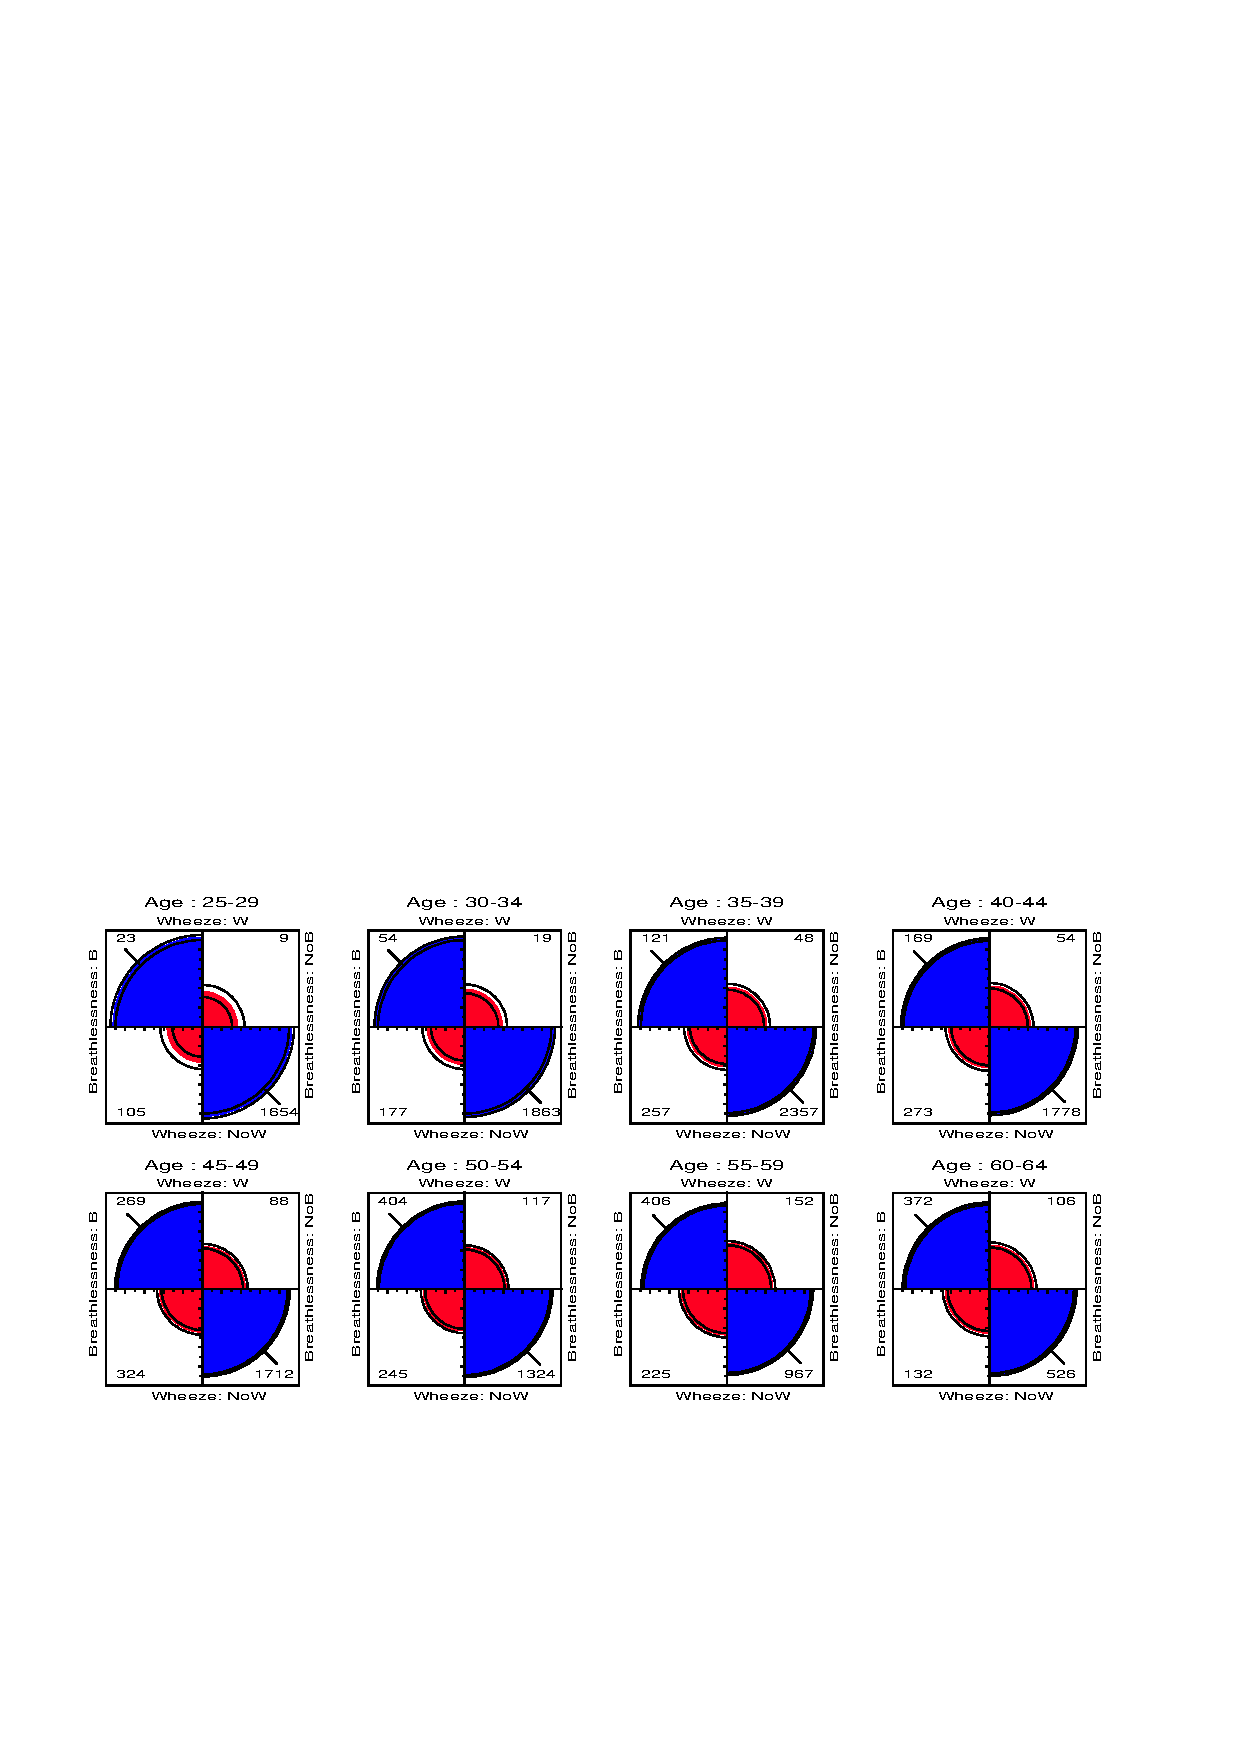
\includegraphics[scale=.8,clip]{ch3/fig/pie2x2wh1}
  \caption[Fourfold display for coal miners data, both margins equated]{Fourfold display for coal miners data, both margins equated.}\label{fig:pie2x2wh1}
\end{figure}
%
\begin{Output}
\caption{Odds ratios and tests of homogeneity of association for coal miners data}\label{out:pie2x2wh}
\small
\verbatiminput{ch3/out/pie2x2wh.out}
\end{Output}

\begin{figure}[htb]
  \centering
  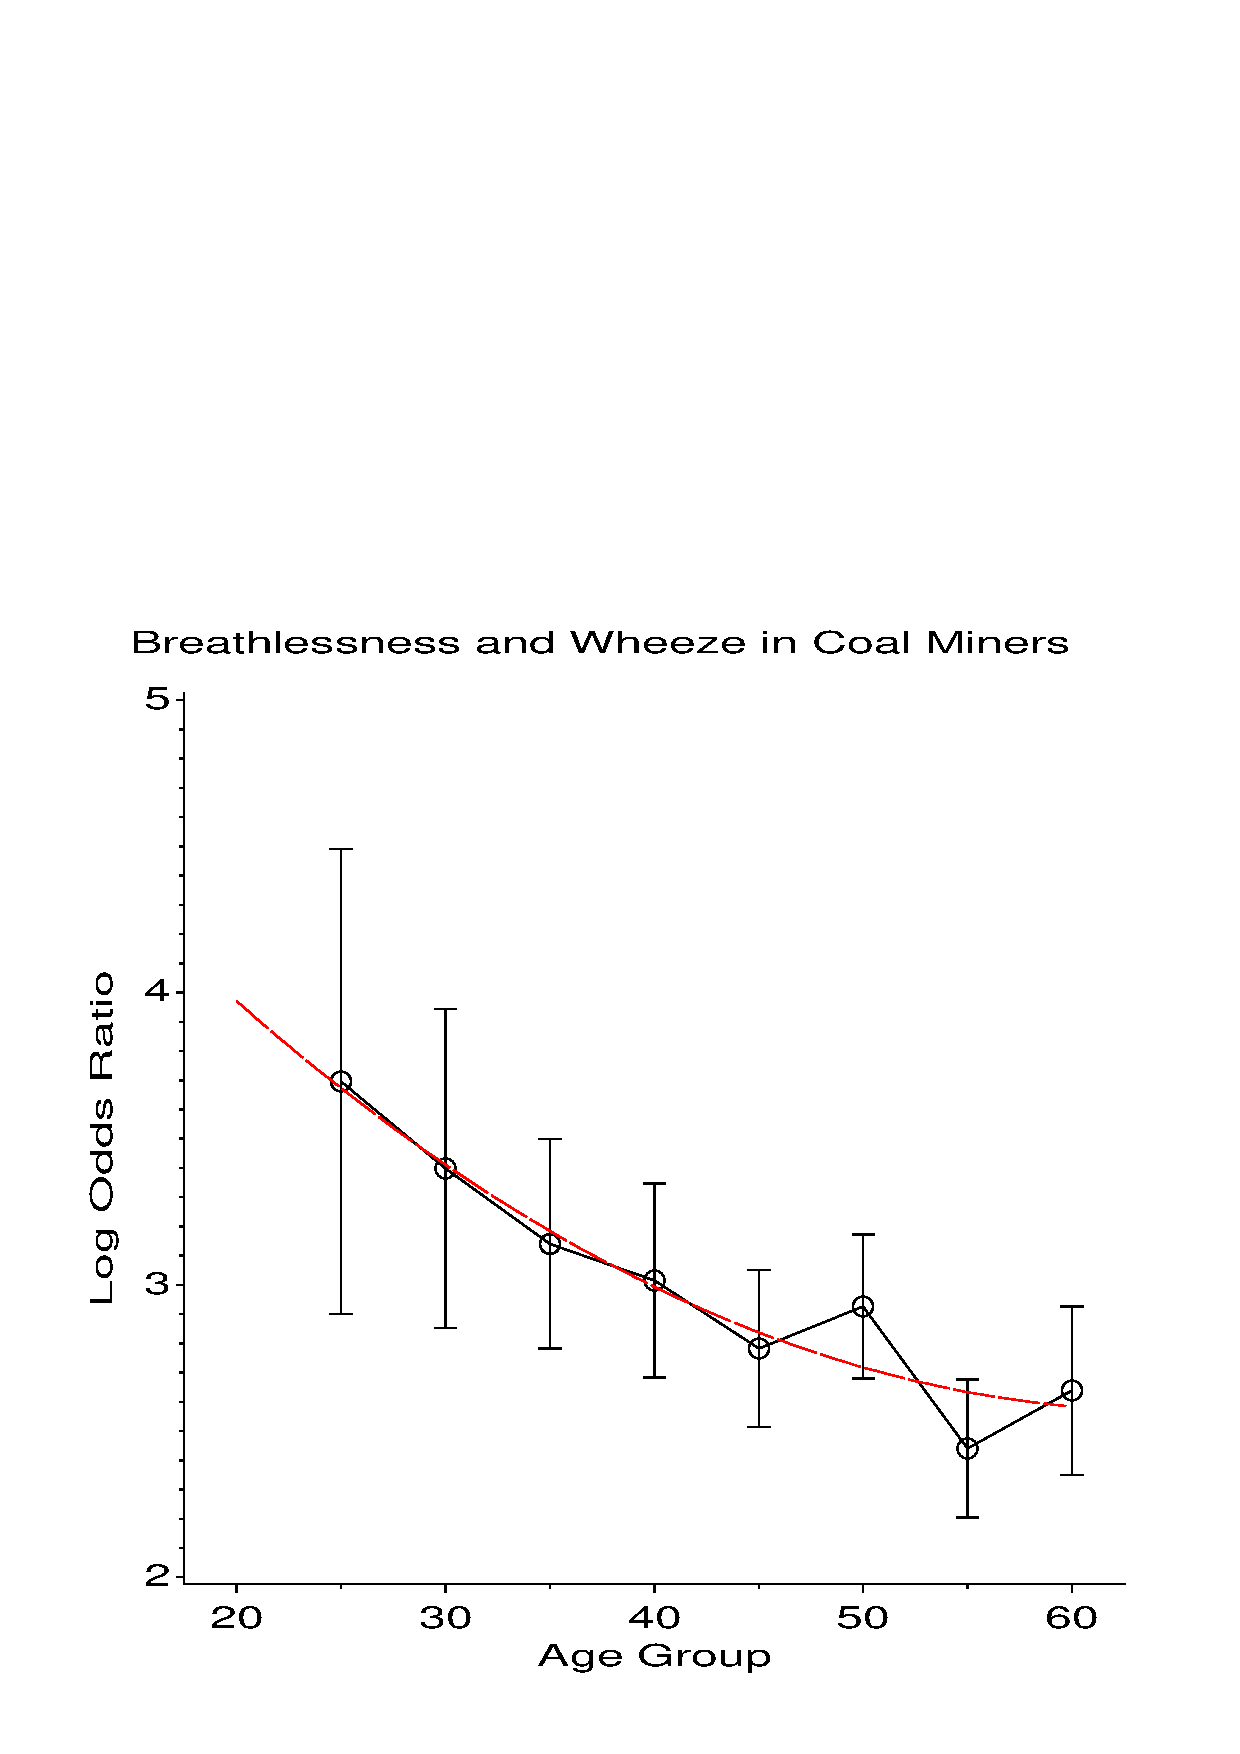
\includegraphics[scale=.6]{ch3/fig/pie2x2wh2}
  \caption[Breathlessness and wheeze in coal miners, odds ratios]{Breathlessness and wheeze in coal miners, log odds plot.  The smooth curve is a quadratic fit.
  Vertical bars give individual 95\% confidence intervals.}\label{fig:pie2x2wh2}
\end{figure}

A more poignant question, however, concerns the prevalence of these
two respiratory symptoms among miners and how these change over age.
The answer is concealed in \figref{fig:pie2x2wh1}, since the
proportion of miners with each symptom are equated in each age group.
This question can be addressed by standardizing the frequencies
to equate the numbers in each stratum (\texttt{std='MAX';}),
which gives the graph shown in \figref{fig:pie2x2wh3}.
If one regards age as reflecting number of years spent working
in coal mines,
this figure shows the sad result of such employment:
the relative frequency of miners with both symptoms steadily
increasing over age.
We return to these data in \exref{ex:ashford},
where we consider a variety of specific
logit models for the prevalence of each symptom
simultaneously with models for their log odds ratio.
\begin{figure}[htb]
  \centering
  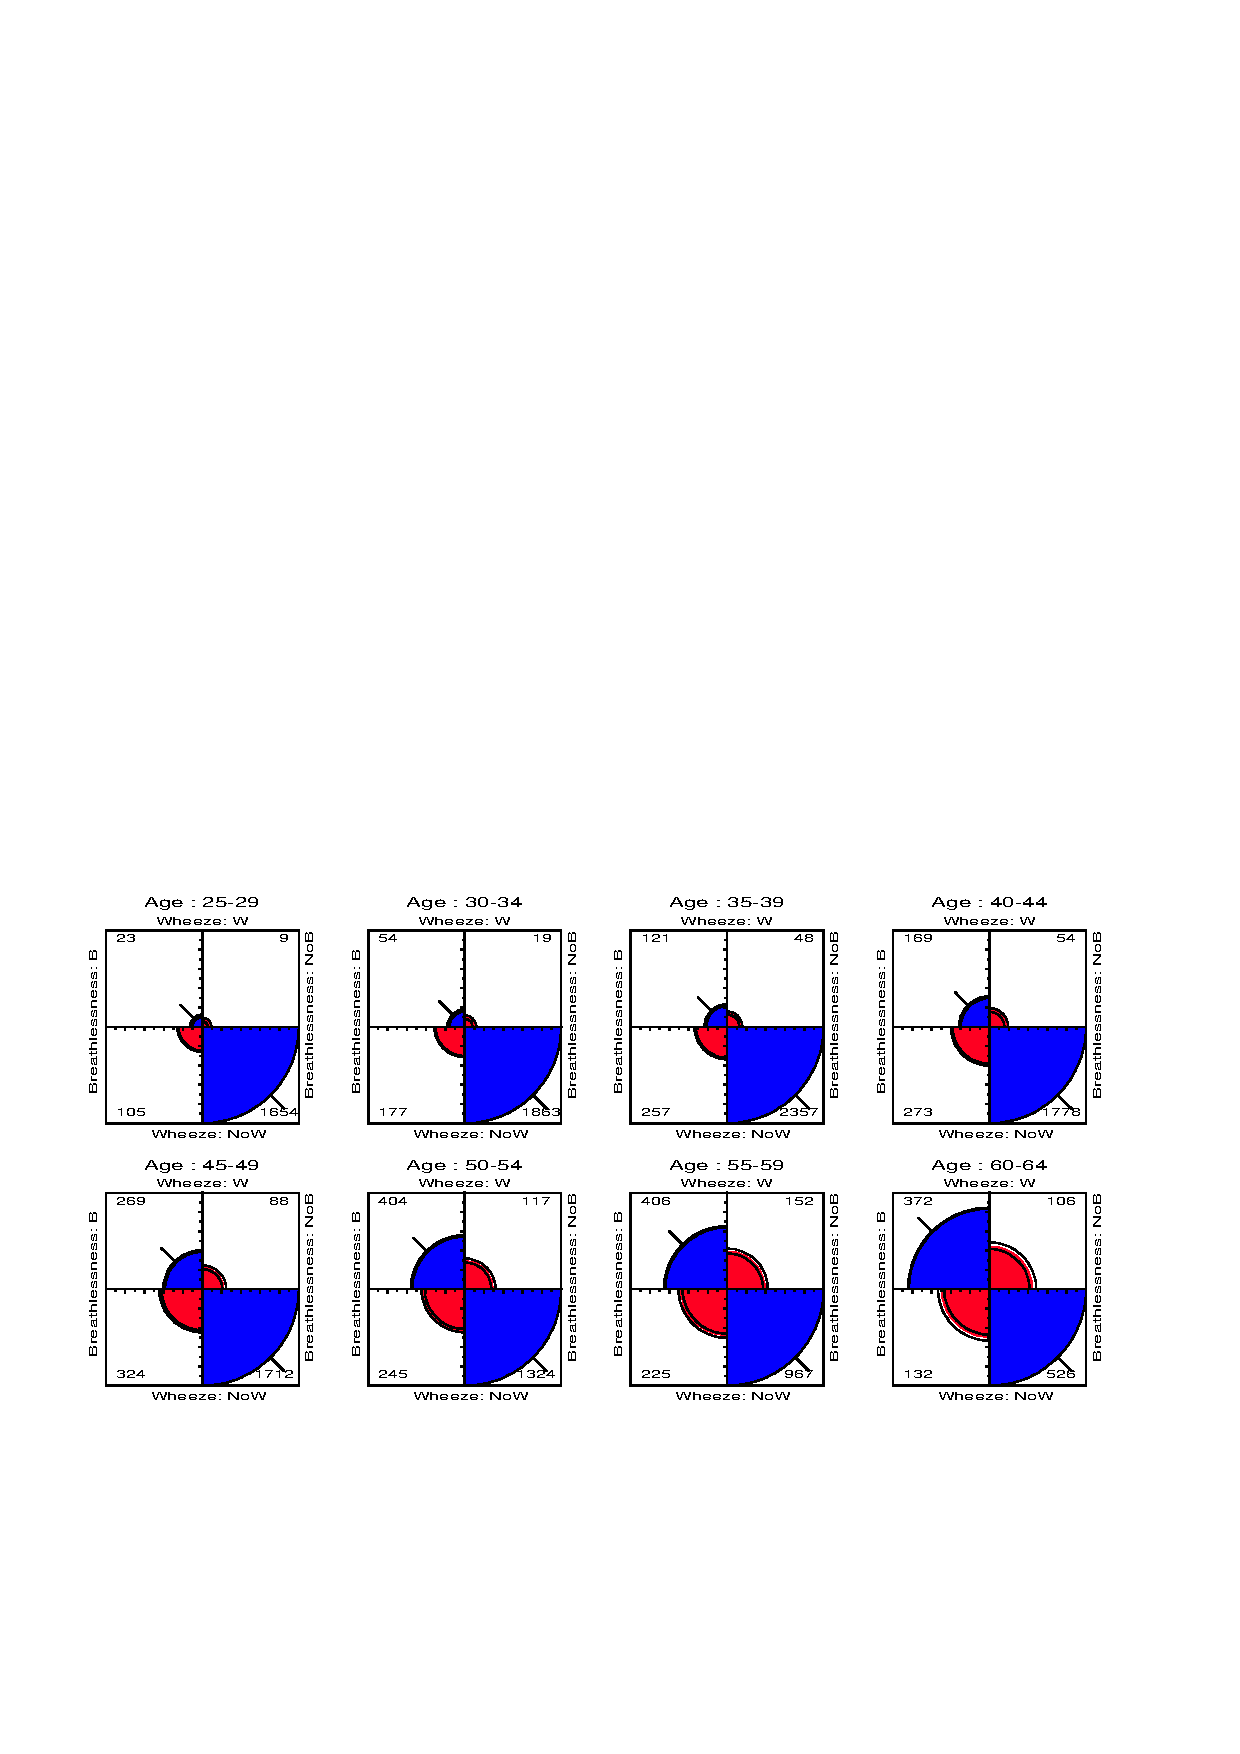
\includegraphics[scale=.8,clip]{ch3/fig/pie2x2wh3}
  \caption[Fourfold display for coal miners data, strata equated]{Fourfold display for coal miners data, strata equated.}\label{fig:pie2x2wh3}
\end{figure}
\end{Example}

%\begin{changebar}
%\begin{Example}[toxaemia0]{Toxaemic symptoms in pregnancy}
In \secref{sec:loglin-multiv}, we examine multivariate models
for two or more categorical responses.
\exref{ex:toxaemia} presents an analysis of data from
\citet{Brown-etal:83}
on the occurrence of two
signs of toxaemia (hypertension and protein urea)
among 13,384 expectant mothers in Bradford, England in their first pregnancy.
The mothers are classified by social class (1--5), and by the
number of cigarettes smoked per day (0, 1--19, or $20+$).

The models presented later describe how both the marginal distributions
of the responses, \emph{and} their association, vary with explanatory variables.
Here, we preview those data with a fourfold display focused on just
the association (odds ratio) between the two binary
response variables, Hypertension and Urea.


%% one figure
\begin{figure}[htb]
  \centering
  \includegraphics[width=\linewidth,clip]{ch3/fig/4ftox.eps}
  \caption[Fourfold display for toxaemia data]{Fourfold display for toxaemia data.  The level of mother's smoking increases from top to bottom;
  mother's social class increases from left to right}%
  \label{fig:4ftox}
\end{figure}

\figref{fig:4ftox} shows the fourfold displays for the 15 combinations
of mother's social class and smoking, with non-smokers in the top row,
and heaviest smokers in the bottom row.
We see that, with one exception (a cell with small total frequency),
the association between presence of hypertension and urea
is positive, and roughly of the same magnitude over the categories
of class, particularly for non- and moderate-smokers.
In \exref{ex:toxaemia} we plot the log odds ratio directly (\figref{fig:tox13}), as well as the log odds for prevalence
of these two symptoms.
\end{Example}

%\end{changebar}
\ixoff{fourfold display}

%\section{Tukey two-way plots}\label{sec:twoway-tukey}


\section{Sieve diagrams}\label{sec:twoway-sieve}
\ixon{sieve diagram}
\epigraph{They consider me to have sharp and penetrating vision because I see
them through the mesh of a sieve.}{Kahlil Gibran}
For two- (and higher-) way \ctabs{}, the
design principles of perception, detection, and comparison
(see \chref{ch:intro})
suggest that we should try to show the observed frequencies
in relation to what we would expect those frequencies to be
under a reasonable null model---for example, the
hypothesis that the row and column variables are unassociated.

To this end, several schemes for representing \ctabs\
graphically are
based on the fact that when the row and column variables are
independent, the estimated expected frequencies, \(m_{ij}\), are
products of the row and column totals (divided by the grand total).
\begin{equation*}
 m_{ij} = \frac{ n_{i+} n_{+j} } { n_{++} }
 \period
\end{equation*}
Then, each cell can be represented by a rectangle whose area shows
the cell frequency, \(n_{ij}\),  or deviation from independence.

For example, for any two-way table, the expected frequencies under independence
can be represented by rectangles whose widths are proportional to the
total frequency in each column, \(n_{+j}\), and whose heights are
proportional to the total frequency in each row, \(n_{i+}\); the area
of each rectangle is then proportional to \(m_{ij}\). \figref{fig:sieve0}
shows the expected frequencies for the hair and eye color
data (\tabref{tab:hairdat}).

This display simply represents the model---what the frequencies would
be if hair color and eye color were independent---not the data.
Note, however, that the rectangles are cross-ruled so that the number of
boxes in each (counting up the fractional bits) equals the expected
frequency with which the cell is labeled, and moreover, the
rulings are equally spaced in all cells.
Hence, cross-ruling the cells to show the observed frequency
would give a data display which implicitly compares observed
and expected frequencies.

\begin{figure}[htb]
  \centering
  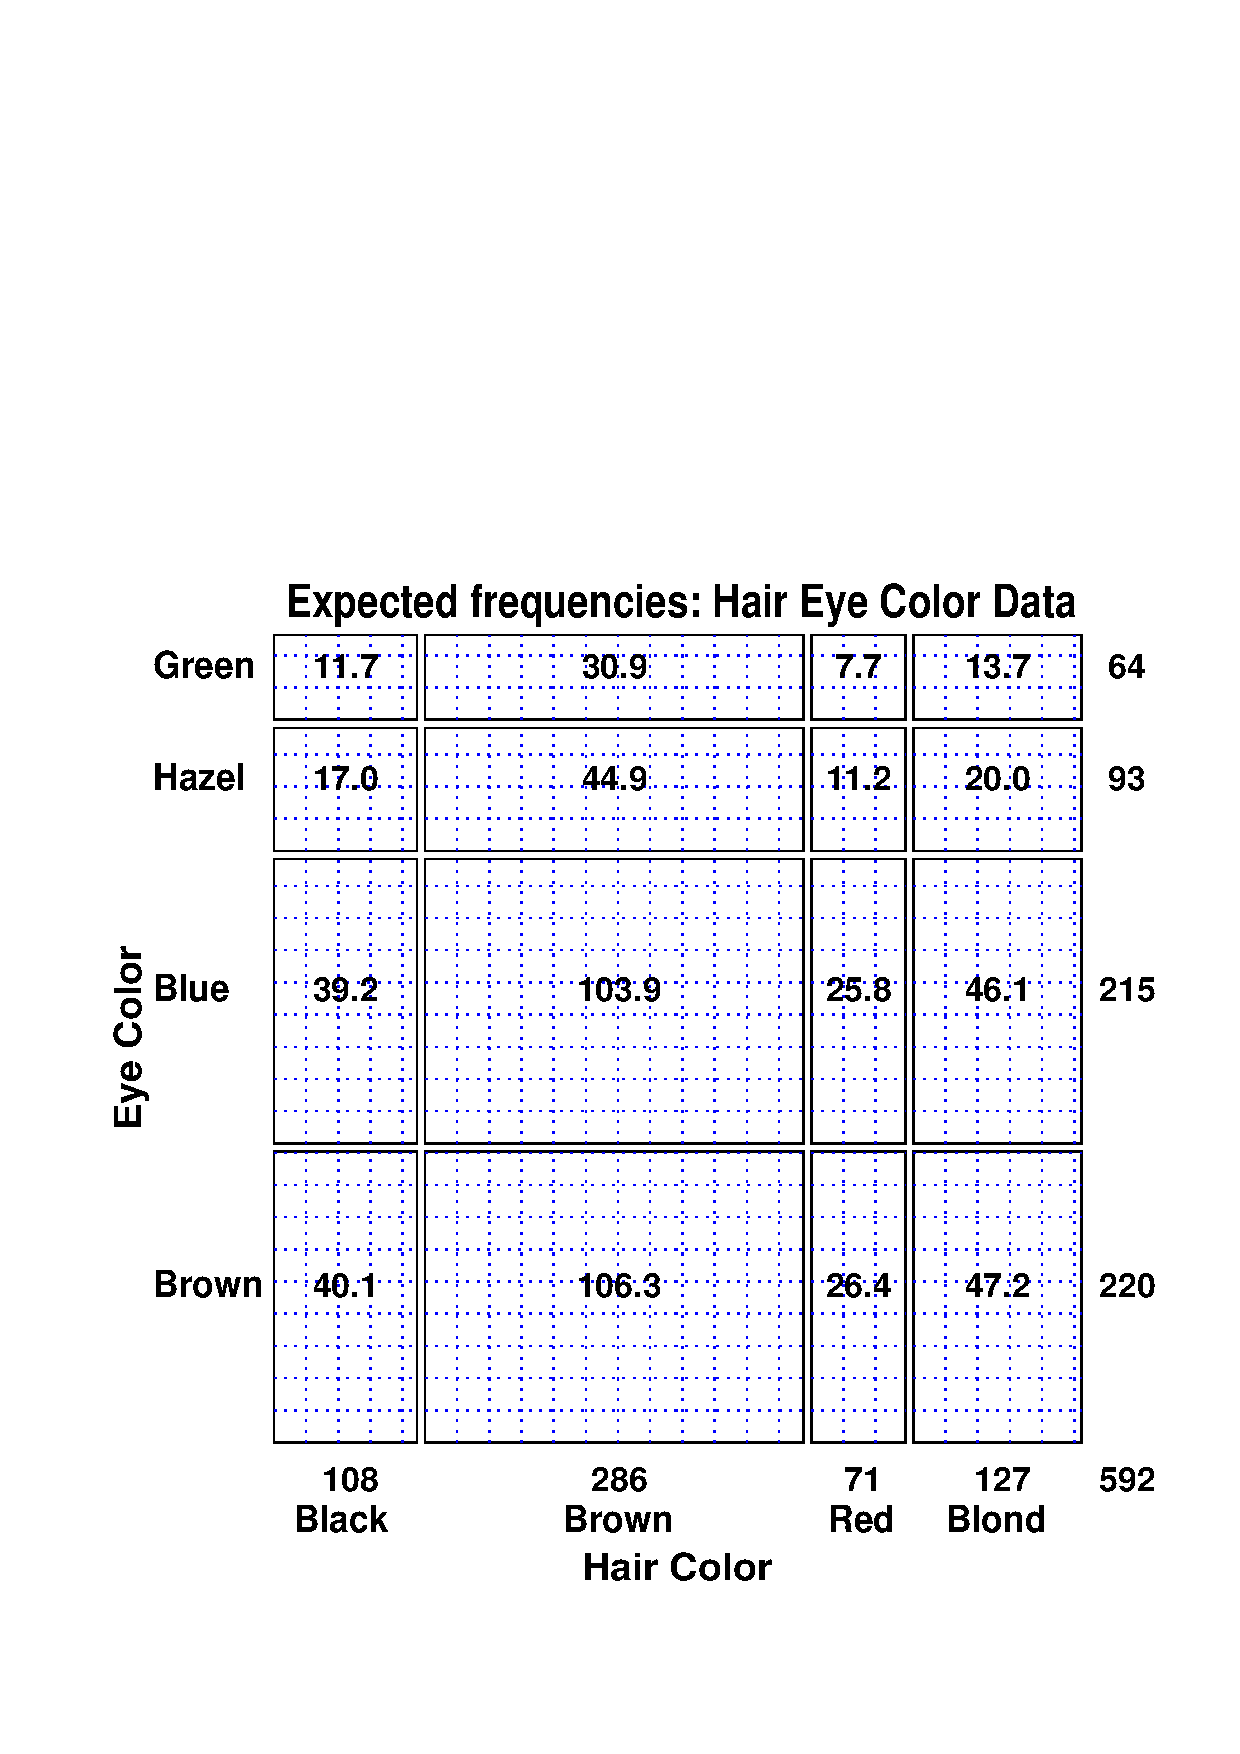
\includegraphics[scale=.5]{ch3/fig/sieve0}
  \caption[Expected frequencies under independence]{Expected frequencies under independence.  Each box has area equal to its expected frequency, and is cross-ruled proportionally to the expected frequency.}\label{fig:sieve0}
\end{figure}


Riedwyl and Sch\"{u}pbach
\citeyear{RiedwylSchupbach:83,RiedwylSchupbach:94}
%(1983, 1994)
proposed a
\glossterm{sieve diagram}
(later called a \glossterm{parquet diagram}) based on
this principle.  In this display the area of each rectangle is
proportional to expected frequency,
as in \figref{fig:sieve0},  but observed frequency is shown by
the number of squares in each rectangle.  Hence, the difference
between observed and expected frequency appears as variations in the density of
shading.
Cells whose observed frequency $n_{ij}$ exceeds the expected $m_{ij}$
appear denser than average.
The pattern of positive and negative deviations from independence
can be more easily seen by
using color, say, red for negative deviations, and blue for positive.%
\footnote{
Positive residuals are also shown by solid lines, negative residuals by broken
lines, so that they may still be distinguished in monochrome versions.}

\begin{Example}[haireye2]{Hair color and eye color}
The sieve diagram for hair color and eye color (\tabref{tab:hairdat})
is shown in
\figref{fig:sieve1}.
The pattern of color and shading shows the high frequency of
blue-eyed blonds and people with brown eyes and dark hair.
People with hazel eyes are also more likely to have red or brown hair,
and those with green eyes more likely to have red or blond hair,
than would be observed under independence.

\begin{figure}[htb]
  \centering
  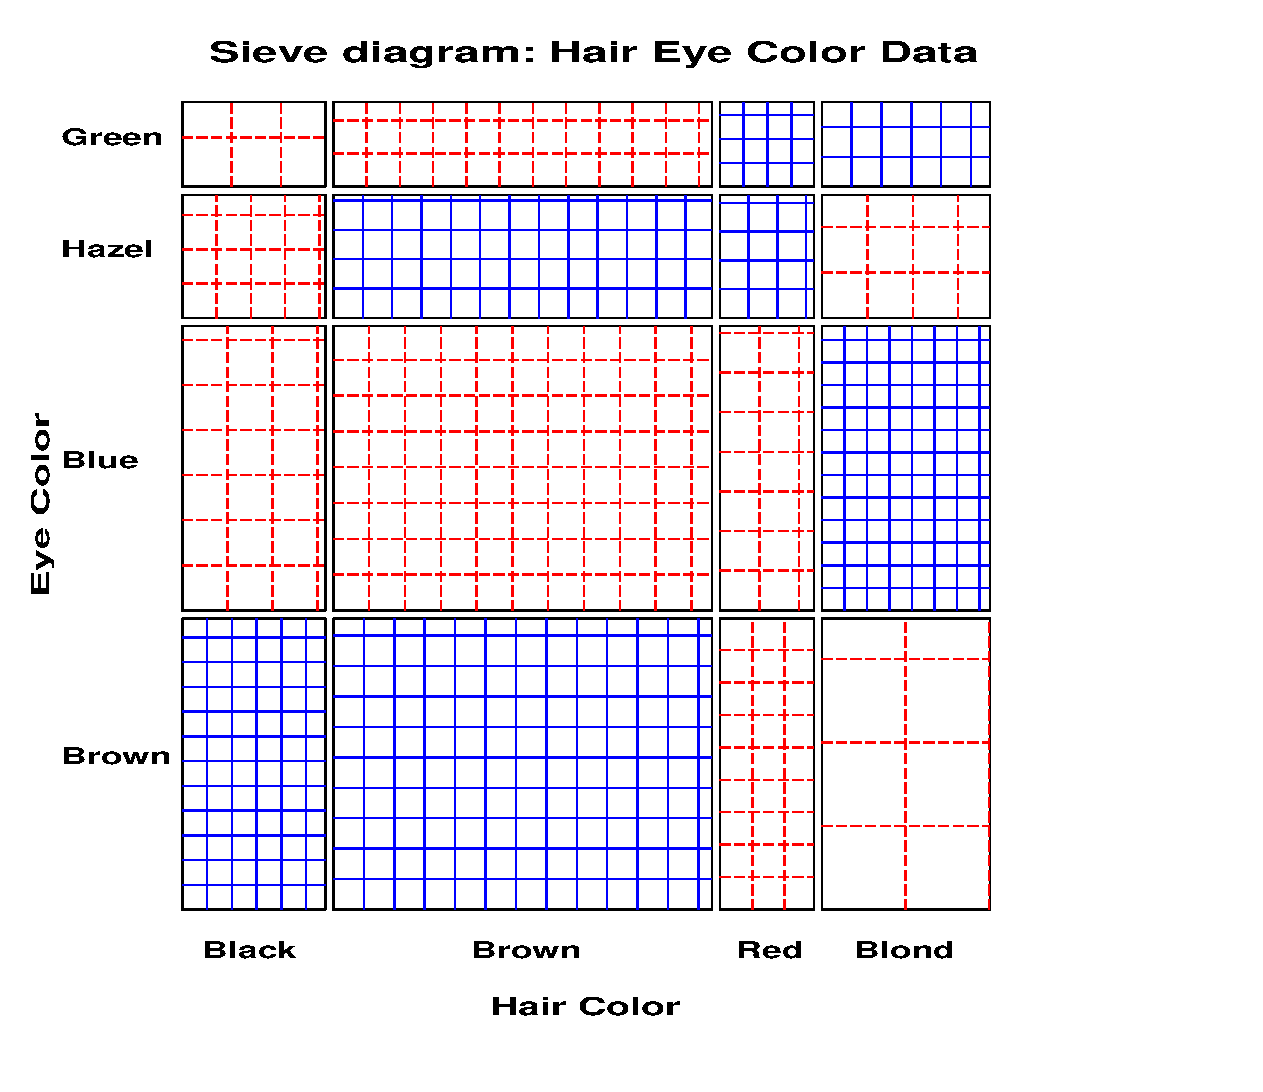
\includegraphics[scale=.5]{ch3/fig/sieve1}
  \caption[Sieve diagram for hair-color, eye-color data]{Sieve diagram for hair-color, eye-color data.  Observed frequencies are equal to the number
  squares in each cell, so departure from independence appears as variations
  in shading density.}\label{fig:sieve1}
\end{figure}
\ixd{hair-eye color}
\end{Example}

\begin{Example}[vision1]{Visual acuity}
\figref{fig:sieve2} shows the sieve diagram for data on visual acuity in a large
sample of women ($n=7477$) aged 30-39, working in the U.K.
Royal Ordnance factories during World War II
(\citet[Table 33.5]{KendallStuart:61},
\citet[p. 284]{Bishop-etal:75}).
For each person, unaided distance vision of each eye was measured
and categorized into four ordered grades.  The data are listed in
\datref{dat:vision}.

The diagonal cells show the obvious:
people tend to have the same visual acuity in both eyes, and there is
strong lack of independence.  The off diagonal cells show a more subtle
pattern which suggests symmetry---the cells below the diagonal
are approximately equally dense as the corresponding cells above the diagonal.
Moreover, the relatively consistent pattern on the diagonals
$\pm 1, \pm 2, \dots$ away from the main diagonals suggests
that the association may be explained in terms of the \emph{difference}
in visual acuity between the two eyes.
These suggestions can be tested by fitting  intermediate models
between the null model of independence (which fits terribly)
and the saturated model (which fits perfectly),
as we shall see later in this book.
A model of quasi-independence, for example (\exref{ex:victims})
ignores the diagonal cells and tests whether independence holds
for the remainder of the table.
%\aunote{Xref?}
\ixd{visual acuity}

\begin{figure}[htb]
  \centering
  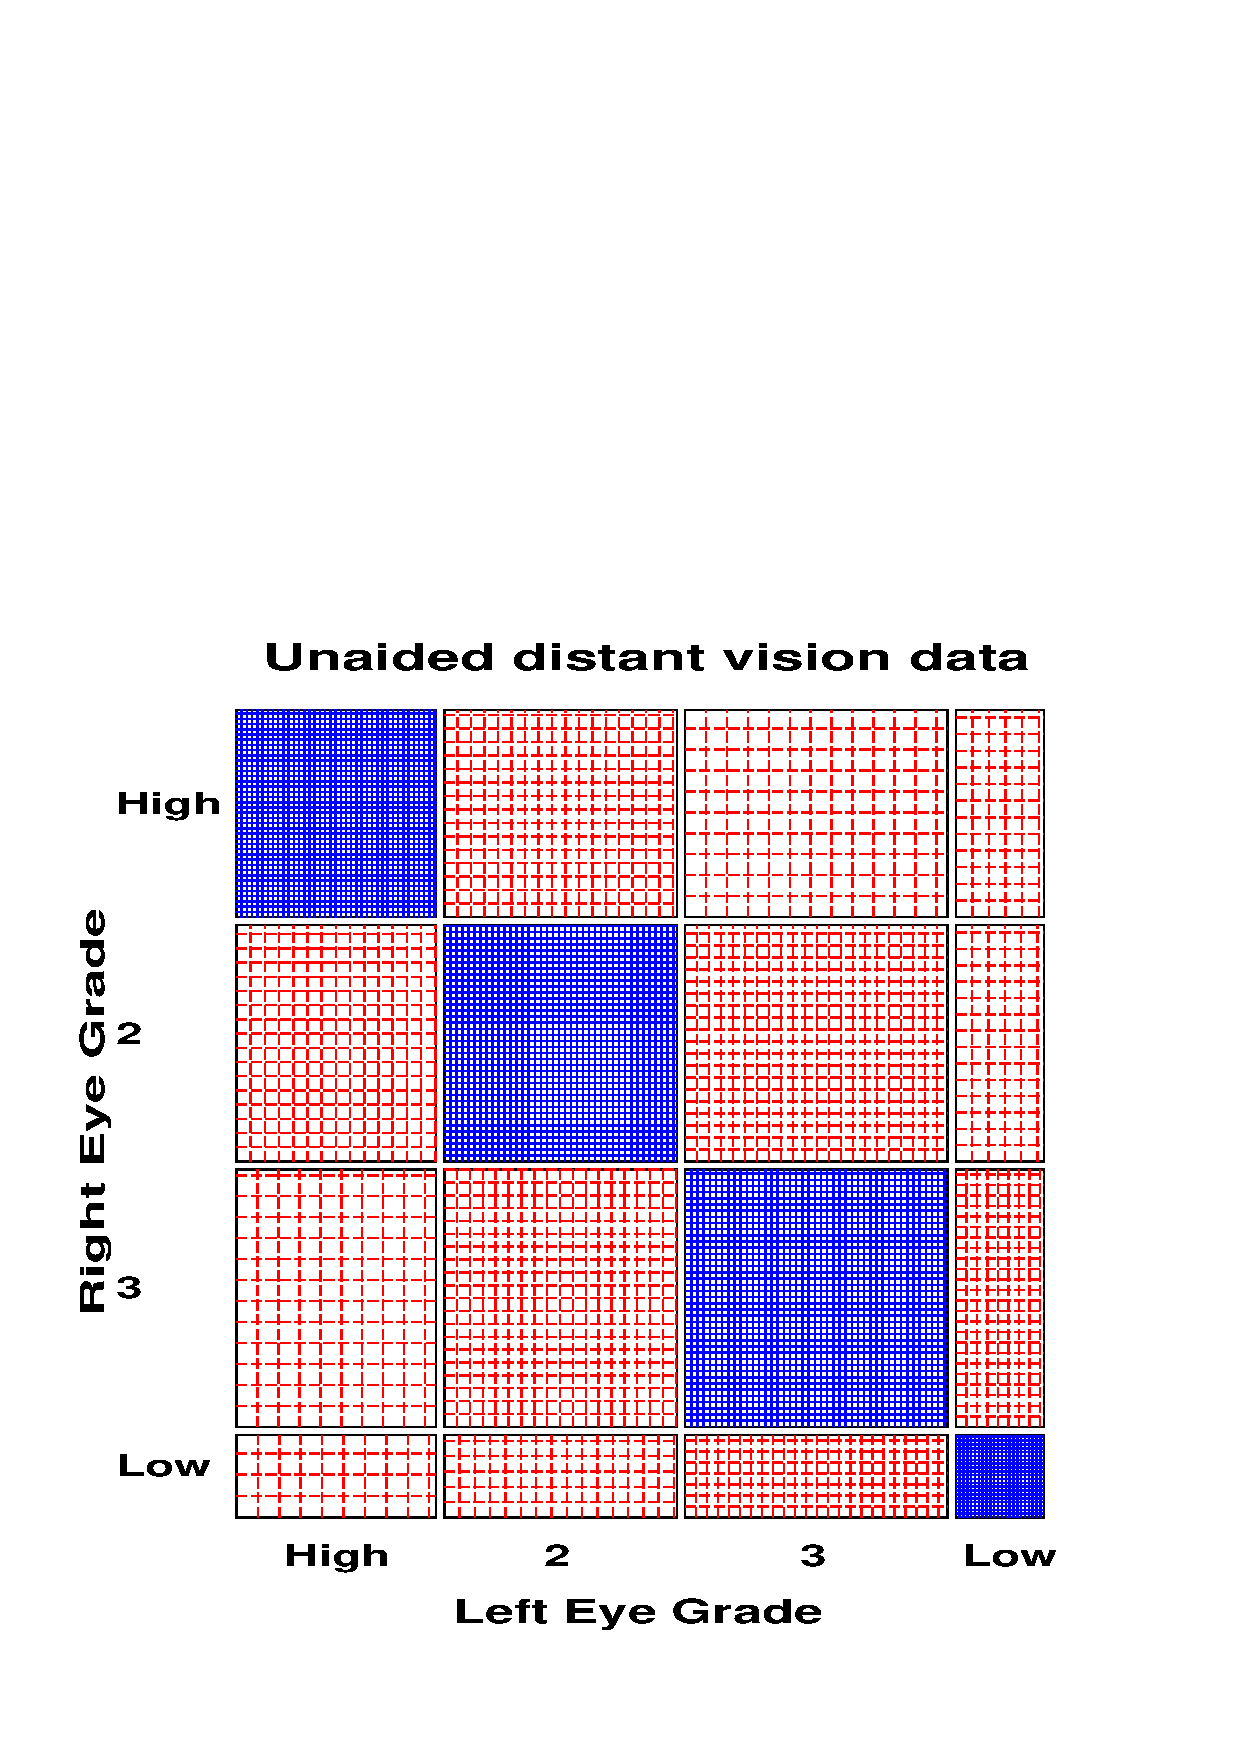
\includegraphics[scale=.5]{ch3/fig/sieve2}
  \caption{Vision classification data for 7477 women}\label{fig:sieve2}
\end{figure}
\end{Example}

\subsection{The \sasprog{SIEVE}}
Sieve diagrams are implemented as a general module in \IML{},
because the calculations and graphics are most easily handled using
matrices.
The program is listed and documented in \macref{mac:sieve}.

To use the program, \texttt{\%include} the \sasprog{SIEVE}
within a \PROC{IML} step.  Then
enter the observed frequencies in an array \texttt{f},
and create a character vector \texttt{vnames} containing
the row and column variable names, and a two-row
character matrix \texttt{lnames} containing the
category labels.
The sieve diagram is produced with the \texttt{sieve} module,
\begin{listing}
run sieve( f, vnames, lnames, title );
\end{listing}
For example, the sieve diagram in \figref{fig:sieve1}
for the hair color eye color data is produced by the
statements below.
Note that the graphics options \texttt{hsize} and \texttt{vsize}
should be set to make the plot square.
%% input: /users/faculty/friendly/sasuser/catdata/sievehair.sas
%% last modified: 05-Jan-98  9:15
\begin{listing}
goptions hsize=7in vsize=7in;
 
filename sieve '~/sasuser/catdata/sieve.sas';
proc iml;
   %include sieve;
   f = \{   5   29  14  16 ,       /* green */
          15   54  14  10 ,       /* hazel */
          20   84  17  94 ,       /* blue  */
          68  119  26   7 \};      /* brown */
 
   vnames = \{'Eye Color' 'Hair Color'\};
   lnames = \{'Green' 'Hazel' 'Blue' 'Brown' ,
             'Black' 'Brown' 'Red'  'Blond'\};
   title  = 'Sieve diagram: Hair Eye Color Data';
   font='hwpsl011';
   run sieve(f, vnames, lnames, title );
quit;
\end{listing}


\subsection{Larger tables}
\ix{interactive coding}
\ix{sieve diagram!interactive coding}
Sieve diagrams are strictly applicable to two-way tables.
However, larger tables may be displayed by representing two or more
table variables interactively along either of the dimensions of a two-way table.
Associations among the variables represented along the rows (or columns)
are not displayed, however associations \emph{between} the row
variable(s) and the column variable(s) are displayed.%
\footnote{The program fits a model where the row variable(s)
are independent of the column variable(s).}

\begin{Example}[berkeley3]{Berkeley admissions}
For example, a sieve diagram may be used to determine if the association
between gender and department is the same across departments
by structuring the three-way table as [Department] by [Admission-Gender],
which gives the plot shown in \figref{fig:sievebrk}
In terms of the \loglin{} models discussed in
the next chapter, this is equivalent to fitting the model
of joint independence, $[D] [AG]$.

\begin{figure}[htb]
  \centering
  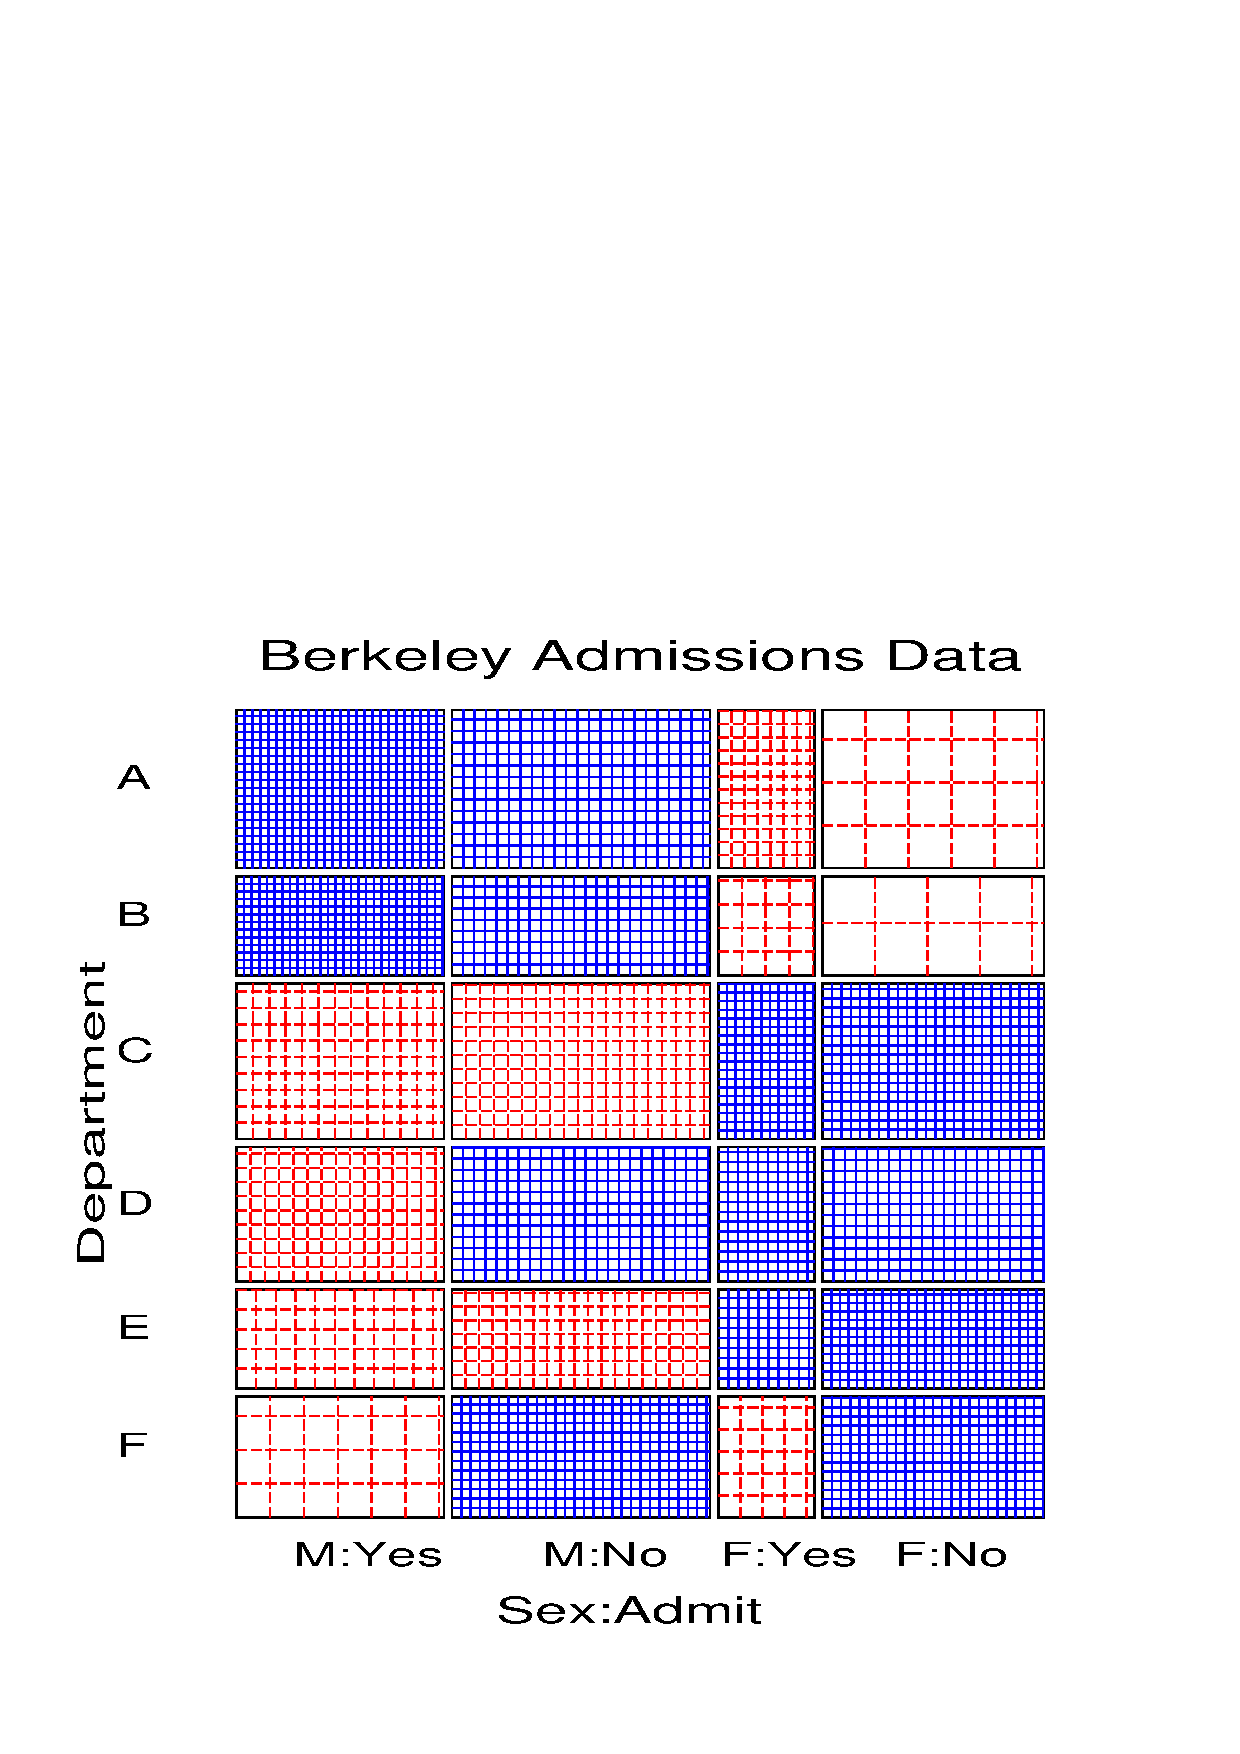
\includegraphics[scale=.5]{ch3/fig/sievebrk}
  \caption[Sieve diagram for Berkeley admissions data]{Sieve diagram for Berkeley admissions data.  The display fits a model (homogeneity) in which the combinations of sex and admission are jointly independent of department.}\label{fig:sievebrk}
\end{figure}

This sieve diagram is produced using the \texttt{sieve} module
as follows:
%% input: /users/faculty/friendly/sasuser/catdata/sievebrk.sas
%% last modified: 07-Jan-98 12:03
\begin{listing}
proc iml;
   %include sieve;
 
   vnames = \{"Department" "Sex:Admit" \};
   lnames = \{ "A" "B" "C" "D" "E" "F",
             "M:Yes" "M:No" "F:Yes"  "F:No" " " " "\};
          /*   Males       Females  */
   table = \{ 512  313      89   19,
             353  207      17    8,
             120  205     202  391,
             138  279     131  244,
              53  138      94  299,
              22  351      24  317\};
 
   font='hwpsl009';
   title  = 'Berkeley Admissions Data';
   run sieve(table, vnames, lnames, title );
quit;
\end{listing}

In this display the widths of the columns show the greater number of
male applicants than female; the greater overall admission rate for
males can be seen by comparing the ratios of widths (M:Yes / M:No) to
that of (F:Yes / F:No).
The marginal frequencies of all applicants to the various departments
are shown by the heights of the rectangles in each row.
Cells with many small squares (in blue)
correspond to those whose observed frequencies are greater than
expected under
independence.  \figref{fig:sievebrk} shows the greater numbers of
male applicants in departments A and B
(whose overall rate of admission is high) and greater numbers of female
applicants in the remaining departments (where the admission rate is low).
\end{Example}
\ixoff{sieve diagram}


\renewcommand{\FileName}{assoc}
\subsection{Nominal factors}
\begin{frame}[fragile]
  \frametitle{Testing Association in Two-Way Tables}
  \begin{block}{\large\bfseries Typical analysis: Nominal factors}
  \end{block}
      \begin{itemize}
	  \item Pearson $\chisq$ (or LR $\chisq$)--- when most expected
	  frequencies $\ge 5$.

\begin{listing}[frame=single]
proc freq;
   weight count;        \sascomment{/* if in frequency form */}
   table factor * response / \sasemph{chisq}; 
\end{listing}

	  \item Exact tests--- small tables, small sample sizes (e.g., Fisher's)

\begin{listing}[frame=single]
proc freq;
   weight count;        \sascomment{/* if in frequency form */}
   table factor * response / \sasemph{chisq};
   \sasemph{exact pchi;}
\end{listing}
	  \end{itemize}
\end{frame}

\begin{frame}[fragile]
  \frametitle{Example: Cholesterol diet and heart disease}
Is there a relation between Hi/Lo cholesterol diet and heart disease?
\vspace{2ex}

\begin{Input}[fontsize=\footnotesize,label=\fbox{\texttt{fat.sas}},baselinestretch=0.8]
title 'Cholesterol diet and heart disease';
data fat;
   input diet $ disease $ count;
datalines;
LoChol  No   6
LoChol  Yes  2
HiChol  No   4
HiChol  Yes 11
;

proc freq data=fat;
  weight count;
  tables diet * disease / chisq nopercent nocol;
  \sasemph{exact pchi};
\end{Input}
\end{frame}

\begin{frame}[fragile]
Standard output:
\begin{Output}[fontsize=\footnotesize,gobble=7,baselinestretch=.7]
                           Table of diet by disease

                     diet      disease

                     Frequency|
                     Row Pct  |No      |Yes     |  Total
                     ---------+--------+--------+
                     HiChol   |      4 |     11 |     15
                              |  26.67 |  73.33 |
                     ---------+--------+--------+
                     LoChol   |      6 |      2 |      8
                              |  75.00 |  25.00 |
                     ---------+--------+--------+
                     Total          10       13       23


                   Statistics for Table of diet by disease

            Statistic                     DF       Value      Prob
            ------------------------------------------------------
            Chi-Square                     1      4.9597    0.0259
            Likelihood Ratio Chi-Square    1      5.0975    0.0240
            Continuity Adj. Chi-Square     1      3.1879    \sasemph{0.0742}

         \sasemph{WARNING}: 50% of the cells have expected counts less than 5. 
                  (Asymptotic) Chi-Square may not be a valid test.
\end{Output}
\begin{itemize*}
  \item The Pearson and LR $\chisq$ tests are \emph{not valid}--- sample size too small
  \item The conservative continuity-adjusted test fails significance
\end{itemize*}
\end{frame}

\begin{frame}[fragile]
\begin{itemize*}
  \item Exact tests are \emph{valid} and significant.
\end{itemize*}
Exact test output:
\begin{Output}[fontsize=\footnotesize,gobble=7,baselinestretch=.8]
            		   Pearson Chi-Square Test
        		  ----------------------------------
        		  Chi-Square                  4.9597
        		  DF                               1
        		  Asymptotic Pr >  ChiSq      0.0259
        		  Exact      Pr >= ChiSq      0.0393


                		 Fisher's Exact Test
        		  ----------------------------------
        		  Cell (1,1) Frequency (F)         4
        		  Left-sided Pr <= F          0.0367
        		  Right-sided Pr >= F         0.9967

        		  Table Probability (P)       0.0334
        		  Two-sided Pr <= P           \sasemph{0.0393}
\end{Output}

\end{frame}

\begin{frame}[fragile]
  \frametitle{Preview: Visualizing association in 2 $\times$ 2 tables}
 \begin{minipage}[c]{.5\linewidth}
  \centering
  \includegraphics[width=.9\linewidth,clip]{fig/fat2}
 \end{minipage}%
 \begin{minipage}[c]{.5\linewidth}
   \begin{itemize}
    \item Fourfold display: area $\sim$ frequency
    \item Color: \blue{blue} ($+$), \red{red}($-$)
    \item Confidence bands: significance of odds ratio
    \item Interp: Hi cholesterol $\rightarrow$ Heart disease
   \end{itemize}
 \end{minipage}
\vspace{1ex}
\begin{listing}[frame=single]
%ffold(data=fat, var=diet disease);
\end{listing}

\end{frame}

\subsection{Ordinal factors and Stratified analyses}
\begin{frame}[fragile]
  \frametitle{Ordinal factors and Stratified analyses}

  \begin{block}{\large\bfseries More powerful CMH tests}
      \begin{itemize*}
	  \item When either the row (factor) or column (response) levels are
	  \alert{ordered}, more specific (CMH = Cochran - Mantel - Haentzel) tests
	  which take order into account have greater power to detect ordered
	  relations.
\begin{listing}[frame=single]
proc freq;
   weight count;
   table factor * response / chisq \sasemph{cmh}; 
\end{listing}
	  \end{itemize*}
  \end{block}
  \begin{block}{\large\bfseries Control for other background variables} 
      \begin{itemize*}
	    \item Stratified analysis tests the association between a main
		factor and response \emph{within}  levels of the control
		variable(s)
		\item Can also test for homogeneous association across strata
\begin{listing}[frame=single]
proc freq;
   weight count;
   table \sasemph{strata} * factor * response / chisq \sasemph{cmh}; 
\end{listing}
	  \end{itemize*}
  \end{block}
\end{frame}

% slide template
\begin{frame}[fragile]
  \frametitle{Example: Arthritis treatment}
  Data on treatment for rheumatoid arthritis \citep{KochEdwards:88}
  \begin{itemize}
	\item {\large\bfseries Ordinal response}: none, some, or marked improvement
	\item {\large\bfseries Factor}:  active treatment vs.\ placebo
	\item{\large\bfseries Strata}:  Sex
  \end{itemize}
\begin{listing}
                      |         Outcome
   ---------+---------+--------------------------+
   Treatment|  Sex    |None    |Some    |Marked  |  Total
   ---------+---------+--------+--------+--------+
   Active   |  Female |      6 |      5 |     16 |     27
            |  Male   |      7 |      2 |      5 |     14
   ---------+---------+--------+--------+--------+
   Placebo  |  Female |     19 |      7 |      6 |     32
            |  Male   |     10 |      0 |      1 |     11
   ---------+---------+--------+--------+--------+
   Total                    42       14       28       84
\end{listing}
\end{frame}

\begin{frame}[fragile]
{\bfseries Overall analysis, ignoring sex}:
\begin{Input}[fontsize=\footnotesize,label=\fbox{\texttt{arthfreq.sas} $\cdots$},baselinestretch=0.8]
title 'Arthritis Treatment: PROC FREQ Analysis';
data arth;
   input sex$ treat$ @;
   do improve = 'None  ', 'Some', 'Marked';
      input count @;
      output;
      end;
datalines;
Female  Active    6  5  16
Female  Placebo  19  7   6
Male    Active    7  2   5
Male    Placebo  10  0   1
;
\sascomment{*-- Ignoring sex;}
proc freq \sasemph{order=data};
   weight count;
   tables treat * improve / \sasemph{cmh} chisq nocol nopercent;
   run;
\end{Input}
{\bfseries Notes}:

\begin{itemize*}

  \item \PROC{FREQ} orders character variables alphabetically (i.e., `Marked', `None', `Some') by
   default.  
  \item To treat the IMPROVE variable as
   ordinal, use \alert{\texttt{order=data}} on the \PROC{FREQ}
   statement.

%  \item The \opt{chisq}{FREQ} gives the usual \(\chi^2\) tests
%   (Pearson, Fisher's, etc.).  The \opt{cmh}{FREQ} requests the
%   \IX{Cochran-Mantel-Haenszel tests} for ordinal variables.
\end{itemize*}
\end{frame}

\begin{frame}[fragile]
\bfseries{Overall analysis, ignoring sex}: Results (\texttt{chisq} option)
\begin{Output}[gobble=2]
             STATISTICS FOR TABLE OF TREAT BY IMPROVE

      Statistic                     DF     Value        Prob
      ------------------------------------------------------
      Chi-Square                     2    13.055       0.001
      Likelihood Ratio Chi-Square    2    13.530       0.001
      Mantel-Haenszel Chi-Square     1    12.859       0.000
      Phi Coefficient                      0.394
      Contingency Coefficient              0.367
      Cramer's V                           0.394
\end{Output}
Cochran-Mantel-Haenszel tests: (\texttt{cmh} option)
\begin{Output}[gobble=4]
               SUMMARY STATISTICS FOR TREAT BY IMPROVE
      Cochran-Mantel-Haenszel Statistics (Based on Table Scores)

    Statistic   Alternative Hypothesis    DF       Value      Prob
    --------------------------------------------------------------
       1        Nonzero Correlation        1      12.859     0.000
       2        Row Mean Scores Differ     1      12.859     0.000
       3        General Association        2      12.900     0.002
\end{Output}
\end{frame}

\subsection{CMH tests for ordinal variables}
\begin{frame}
\frametitle{CMH tests for ordinal variables}
Three types of test:
  \begin{block}{\large\bfseries Non-zero correlation} 
	  \begin{itemize*}
	  \item Use when \emph{both} row and column variables are ordinal.
	  \item CMH \(\chi^2 = ( N - 1) r^2\), assigning scores (1, 2, 3, ...)
	  \item most powerful for \emph{linear} association
	  \end{itemize*}
  \end{block}
  \begin{block}{\large\bfseries Row Mean Scores Differ} 
      \begin{itemize*}
	  \item Use when only \emph{column} variable is ordinal
	  \item Analogous to the Kruskal-Wallis non-parametric test (ANOVA on rank scores)
	  \item Ordinal variable must be listed \alert{last} in the \texttt{TABLES} statement
       \end{itemize*}
  \end{block}
  \begin{block}{\large\bfseries General Association} 
      \begin{itemize*}
	  \item Use when \emph{both} row and column variables are nominal.
	  \item Similar to overall Pearson \(\chi^2\) and Likelihood Ratio \(\chi^2\).
       \end{itemize*}
  \end{block}
\end{frame}

\begin{frame}[fragile,t]
  \frametitle{Sample CMH Profiles}
  \boldital{Only general association:}
\begin{listing}
        | b1    | b2    | b3    | b4    | b5    |  Total  Mean
--------+-------+-------+-------+-------+-------+
  a1    |     0 |    15 |    25 |    15 |     0 |     55   3.0
  a2    |     5 |    20 |     5 |    20 |     5 |     55   3.0
  a3    |    20 |     5 |     5 |     5 |    20 |     55   3.0
--------+-------+-------+-------+-------+-------+
Total        25      40      35      40      25      165
\end{listing}
\vspace{2ex}
Output:
\begin{Output}[gobble=4]
      Cochran-Mantel-Haenszel Statistics (Based on Table Scores)

    Statistic   Alternative Hypothesis    DF       Value      Prob
    --------------------------------------------------------------
       1        Nonzero Correlation        1       0.000     1.000
       2        Row Mean Scores Differ     2       0.000     1.000
       3        General Association        8      91.797     \sasemph{0.000}
\end{Output}
\end{frame}

\begin{frame}[fragile,t]
  \frametitle{Sample CMH Profiles}
\boldital{Linear Association:}

\begin{listing}
        | b1    | b2    | b3    | b4    | b5    |  Total   Mean
--------+-------+-------+-------+-------+-------+
  a1    |     2 |     5 |     8 |     8 |     8 |     31   3.48
  a2    |     2 |     8 |     8 |     8 |     5 |     31   3.19
  a3    |     5 |     8 |     8 |     8 |     2 |     31   2.81
  a4    |     8 |     8 |     8 |     5 |     2 |     31   2.52
--------+-------+-------+-------+-------+-------+
Total        17      29      32      29      17      124
\end{listing}
\vspace{2ex}
Output:
\begin{Output}[gobble=4]
      Cochran-Mantel-Haenszel Statistics (Based on Table Scores)

    Statistic   Alternative Hypothesis    DF       Value      Prob
    --------------------------------------------------------------
       1        Nonzero Correlation        1      10.639     \sasemph{0.001}
       2        Row Mean Scores Differ     3      10.676     \sasemph{0.014}
       3        General Association       12      13.400     0.341
\end{Output}
\end{frame}

\begin{frame}
  \frametitle{Sample CMH Profiles}
\boldital{Visualizing Association:} Sieve diagrams

\vspace{2ex}
 \begin{minipage}[b]{.5\linewidth}
  \centering
  \includegraphics[width=.95\linewidth]{fig/cmhdemo1}
%  \caption{General association (sieve diagram)}\label{fig:cmhdemo1}
 \end{minipage}%
 \begin{minipage}[b]{.5\linewidth}
  \centering
  \includegraphics[width=.95\linewidth]{fig/cmhdemo2}
%  \caption{Linear association (sieve diagram)}\label{fig:cmhdemo2}
 \end{minipage}
\end{frame}

\subsection{Stratified analysis}
\begin{frame}[fragile]
  \frametitle{Stratified analysis}
  \begin{block}{\large\bfseries Overall analysis}
      \begin{itemize*}
	  \item ignores other variables (like sex), by collapsing over them
	  \item risks losing important interactions (e.g., different associations for M \& F)
	  \end{itemize*}
  \end{block}
  \begin{block}{\large\bfseries Stratified analysis}
      \begin{itemize*}
	  \item controls for the effects of one or more background variables
	  \item list stratification variable(s) \emph{first} on the \texttt{TABLES} statement
\begin{listing}[frame=single]
proc freq;
   tables \sasemph{age * sex} * treat * improve;
\end{listing}
	  \end{itemize*}
  \end{block}
  \begin{block}{Looking forward: Loglinear models}
      \begin{itemize*}
	  \item allow more general hypotheses to be stated and tested
	  \item closer connection between testing and visualization (\alert{how} are variables associated)
 	  \end{itemize*}
 \end{block}
\end{frame}

\begin{frame}[fragile]
  \frametitle{Stratified analysis}
The statements below request a stratified analysis with CMH tests,
controlling for sex.

\begin{Input}[fontsize=\footnotesize,label=\fbox{$\cdots$ \texttt{arthfreq.sas} $\cdots$},baselinestretch=0.8,firstnumber=20]
\sascomment{*-- Stratified analysis, controlling for sex;}
proc freq order=data;
   weight count;
   tables sex * treat * improve / cmh chisq nocol nopercent;
   run;
\end{Input}
$\rightarrow$ separate tables (partial tests) for Females and Males
\begin{Output}
       STATISTICS FOR TABLE 1 OF TREAT BY IMPROVE
               CONTROLLING FOR SEX=Female

 Statistic                     DF     Value        Prob
 ------------------------------------------------------
 Chi-Square                     2    11.296       0.004
 Likelihood Ratio Chi-Square    2    11.731       0.003
 Mantel-Haenszel Chi-Square     1    10.935       0.001
  ...
\end{Output}
\begin{itemize*}
\item Strong association between TREAT and IMPROVE for females
\end{itemize*}
\end{frame}

\begin{frame}[fragile]
Males:
\begin{Output}
       STATISTICS FOR TABLE 2 OF TREAT BY IMPROVE
                CONTROLLING FOR SEX=Male

 Statistic                     DF     Value        Prob
 ------------------------------------------------------
 Chi-Square                     2     4.907       0.086
 Likelihood Ratio Chi-Square    2     5.855       0.054
 Mantel-Haenszel Chi-Square     1     3.713       0.054
  ...

\sasemph{WARNING}:  67% of the cells have expected counts less
           than 5. Chi-Square may not be a valid test.
\end{Output}
\begin{itemize*}
\item Weak association between TREAT and IMPROVE for males
\item Sample size $N=29$ for males is small
\end{itemize*}

\end{frame}

\begin{frame}[fragile]
\frametitle{Stratified tests}
  \begin{itemize*}
    \item Individual (\emph{partial}) tests are followed by a \emph{conditional} test,
	controlling for strata (SEX)
	\item These tests {\bf do not} require large sample size in the individual
strata--- just a large total sample size.
    \item They \emph{assume}, but do not \emph{test} that the association is the
	same for all strata.
  \end{itemize*}

\begin{Output}[gobble=6]
                 SUMMARY STATISTICS FOR TREAT BY IMPROVE
                           CONTROLLING FOR SEX

        Cochran-Mantel-Haenszel Statistics (Based on Table Scores)

      Statistic   Alternative Hypothesis    DF       Value      Prob
      --------------------------------------------------------------
         1        Nonzero Correlation        1      14.632     0.000
         2        Row Mean Scores Differ     1      14.632     0.000
         3        General Association        2      14.632     0.001
\end{Output}

\end{frame}

\subsection{Homogeneity of association}
\begin{frame}[fragile]
  \frametitle{Homogeneity of association}
  \begin{itemize}
	\item Is the association between the primary table variables the same over all strata?
	\item 2 $\times$ 2 tables: $\rightarrow$ Equal odds ratios across all strata?
      \begin{itemize*}
	  \item \PROC{FREQ}: \texttt{MEASURES} option on \texttt{TABLES} statement $\rightarrow$ Breslow-Day test
\begin{listing}[frame=single]
 proc freq;
    tables strata * factor * response / \sasemph{measures cmh} ;
\end{listing}

	  \end{itemize*}
	\item Larger tables: Use \PROC{CATMOD} to test for \emph{no three-way association} 
       \begin{itemize*} 
        \item $\equiv$ \alert{same} association for the primary factor \& response variables $\forall$ strata
        \item $\equiv$\loglin\ model: [Strata Factor] [Strata Response] [Factor Response]
\begin{listing}[frame=single]
 proc catmod;
    ...
    loglin strata | factor | response @2;
\end{listing}
       \end{itemize*}
  \end{itemize}
\end{frame}

\begin{frame}[fragile]
  \frametitle{Homogeneity of association: Example}
  \begin{itemize}
	\item Arthritis data: homogeneity $\leftrightarrow$ no 3-way sex * treatment * outcome association
      \begin{itemize*}
	  \item $\equiv$ \loglin\ model: [SexTreat] [SexOutcome] [TreatOutcome] 
	  \item $\equiv$ \texttt{loglin sex|treat|improve@2} for \PROC{CATMOD}
	  \item Zero frequencies: \PROC{CATMOD} treats as ``structural zeros'' by default; recode if necessary.
	  \end{itemize*}
  \end{itemize}

\begin{Input}[fontsize=\footnotesize,label=\fbox{$\cdots$ \texttt{arthfreq.sas}},baselinestretch=0.8,firstnumber=26]
title2 'Test homogeneity of treat*improve association';
data arth;
   set arth;
   if count=0 then count=1E-20;   \sascomment{*-- sampling zeros;}
proc catmod order=data;
   weight count;
   model sex * treat * improve = _response_ / ml ;
   loglin \sasemph{sex|treat|improve @2} / title='No 3-way association';
run;
   loglin sex treat|improve   / title='No Sex Associations';
\end{Input}
\end{frame}

\begin{frame}[fragile]
  \frametitle{Homogeneity of association: Example}
  \begin{itemize*}
  \item the likelihood ratio \(\chi^2\) (the
badness-of-fit for the No 3-Way model) is the test for homogeneity
  \item clearly non-significant $\rightarrow$
treatment-outcome association can be considered to be the same for
men and women.
  \end{itemize*}
\begin{Output}[baselinestretch=0.75]
      Test homogeneity of treat*improve association
                   No 3-way association
      MAXIMUM-LIKELIHOOD ANALYSIS-OF-VARIANCE TABLE

    Source                   DF   Chi-Square      Prob
    --------------------------------------------------
    SEX                       1        14.13    0.0002
    TREAT                     1         1.32    0.2512
    SEX*TREAT                 1         2.93    0.0871
    IMPROVE                   2        13.61    0.0011
    SEX*IMPROVE               2         6.51    0.0386
    TREAT*IMPROVE             2        13.36    0.0013

    \sasemph{LIKELIHOOD RATIO}          2         1.70    \sasemph{0.4267}
\end{Output}
  \begin{itemize*}
  \item But, associations of \texttt{SEX*TREAT} and \texttt{SEX*IMPROVE}
  are both small.
  \item Suggests stronger model of homogeneity, [Sex] [TreatOutcome],
  tested by \texttt{loglin sex treat|improve;} statement.
  \end{itemize*}

\end{frame}

\begin{frame}[fragile]
  \frametitle{Homogeneity of association: Reduced model}
\begin{Input}[fontsize=\footnotesize,label=\fbox{$\cdots$ \texttt{arthfreq.sas}},baselinestretch=0.8,firstnumber=30]
proc catmod order=data;
   weight count;
   model sex * treat * improve = _response_ / ml ;
   loglin sex|treat|improve@2 / title='No 3-way association';
run;
   loglin \sasemph{sex treat|improve}   / title='No Sex Associations';
\end{Input}
Output:
\begin{Output}[baselinestretch=0.75]
                   No Sex Associations
      MAXIMUM-LIKELIHOOD ANALYSIS-OF-VARIANCE TABLE

    Source                   DF   Chi-Square      Prob
    --------------------------------------------------
    SEX                       1        12.95    0.0003
    TREAT                     1         0.15    0.6991
    IMPROVE                   2        10.99    0.0041
    TREAT*IMPROVE             2        12.00    0.0025

    LIKELIHOOD RATIO          5         9.81    \sasemph{0.0809}
\end{Output}
  \begin{itemize*}
  \item Fits reasonably well
  \item How to interpret?
  \end{itemize*}

\end{frame}

\begin{frame}
  \frametitle{Homogeneity of association}
\boldital{Visualizing Association:} Mosaic displays

\vspace{2ex}
 \begin{minipage}[b]{.5\linewidth}
  \centering
  \includegraphics[width=.95\linewidth,clip]{fig/arthmos1} \\ Baseline model
 \end{minipage}%
 \begin{minipage}[b]{.5\linewidth}
  \centering
  \includegraphics[width=.95\linewidth,clip]{fig/arthmos2}  \\ Reduced model
 \end{minipage}

\end{frame}

\endinput

% slide template
\begin{frame}
  \frametitle{}
  \begin{itemize}
	\item{\large\bfseries }
      \begin{itemize*}
	  \item 
    	\begin{itemize*}
		\item 
		\item 
		\end{itemize*}
	  \item 
	  \end{itemize*}
	\item{\large\bfseries }
	\item{\large\bfseries }
  \end{itemize}
\end{frame}


\renewcommand{\FileName}{agree}
% slide template
\begin{frame}
  \frametitle{Observer Agreement}
  \begin{itemize}
	\item {\large\bfseries Inter-observer agreement} often used as to assess 
reliability of a subjective classification or assessment procedure
      \begin{itemize*}
        \item $\rightarrow$ square table, Rater 1 x Rater 2
	    \item Levels: diagnostic categories (normal, mildly impaired, severely
		impaired)
	  \end{itemize*}
	\item{\large\bfseries Agreement vs.\ Association:} Ratings can be strongly associated 
	without strong agreement
	\item{\large\bfseries Marginal homogeneity:}  Different frequencies of
	category use by raters affects measures of agreement
	\item{\large\bfseries Measures of Agreement:}
      \begin{itemize*}
	  \item Intraclass correlation:  ANOVA framework--- multiple raters!
	  \item Cohen's $\kappa$: compares the observed agreement, \(P_o  =
\sum p_{ii}\), to agreement expected by chance if the two observer's
ratings were independent, \(P_c = \sum p_{i+} \,  p_{+i}\).
  \begin{equation*} \label{eq:kappa}
  \kappa =  \frac{ P_o - P_c } { 1 - P_c }
  \end{equation*}
      \end{itemize*}
  \end{itemize}
\end{frame}

\subsection[Cohen's kappa]{Cohen's kappa}
\begin{frame}[fragile]
  \frametitle{Cohen's $\kappa$}
  \begin{itemize*}
      \item Properties of Cohen's $\kappa$:
    	\begin{itemize*}
		\item perfect agreement: \(\kappa = 1\)
		\item minimum \(\kappa\) may be \(< 0\); lower bound depends on marginal
       totals
	    \item Unweighted $\kappa$: counts only diagonal cells (same
       category assigned by both observers).
	    \item Weighted $\kappa$: allows partial credit for near agreement.
		(Makes sense only when the categories are \emph{ordered}.)
		\end{itemize*}
	  \item Weights:  
    	\begin{itemize*}
			\item Cicchetti-Alison (inverse integer spacing) vs.\
	  		\item Fleiss-Cohen (inverse square spacing)
 		\end{itemize*}
 \end{itemize*}

\begin{Output}[fontsize=\footnotesize]
       Integer Weights                 Fleiss-Cohen Weights
   1     2/3     1/3       0          1     8/9     5/9      0
 2/3       1     2/3     1/3        8/9       1     8/9    5/9
 1/3     2/3       1     2/3        5/9     8/9       1    8/9
   0     1/3     2/3       1          0     5/9     8/9      1
\end{Output}

\end{frame}

\begin{frame}[fragile]
  \frametitle{Cohen's $\kappa$: Example}
The table below summarizes responses of 91
married couples to a questionnaire item,

\begin{quote}
Sex is fun for me and my partner (a) Never or occasionally, (b)
fairly often, (c) very often, (d) almost always.  
\end{quote}
\vspace{2em}

\begin{Output}
              --------- Wife's Rating --------
Husband's     Never   Fairly     Very   Almost
Rating          fun    often    Often   always    |   SUM    
--------------------------------------------------+-------
Never fun         \sasemph{7}        7        2        3    |    19
Fairly often      2        \sasemph{8}        3        7    |    20
Very often        1        5        \sasemph{4}        9    |    19
Almost always     2        8        9       \sasemph{14}    |    33
--------------------------------------------------+-------
SUM              12       28       18       33    |    91    
\end{Output}
\end{frame}

\begin{frame}[fragile]
  \frametitle{Computing $\kappa$ with SAS}
  \begin{itemize}
	\item \PROC{FREQ}: Use \texttt{AGREE} option on \texttt{TABLES} statement
      \begin{itemize*}
	  \item Gives both unweighted and weighted $\kappa$ (default: CA weights)
	  \item \texttt{AGREE (wt=FC)} uses Fleiss-Cohen weights
	  \item Bowker's \citep{Bowker:48} test of symmetry: $H_0 : p_{ij} = p_{ji}$
	  \end{itemize*}
  \end{itemize}

\vspace{2ex}
\begin{Input}[fontsize=\footnotesize,label=\fbox{\texttt{kappa3.sas}},baselinestretch=0.8]
title 'Kappa for Agreement';
data fun;
   do Husband = 1 to 4;
   do Wife    = 1 to 4;
      input count @@;
      output;
      end; end;
datalines;
 7     7     2      3
 2     8     3      7
 1     5     4      9
 2     8     9     14
;
proc freq;
  weight count;
  tables Husband * Wife / noprint \sasemph{agree};      \sascomment{/* default: CA weights*/}
  tables Husband * Wife / noprint \sasemph{agree(wt=FC)};
\end{Input}
\end{frame}

\begin{frame}[fragile]
  \frametitle{Computing $\kappa$ with SAS}
Output (CA weights):
\begin{Output}[baselinestretch=0.8,gobble=3]
              Statistics for Table of Husband by Wife

                         Test of Symmetry
                      -----------------------
                      Statistic (S)    3.8778
                      DF                    6
                      Pr > S           0.6932

                          Kappa Statistics
 
    Statistic          Value       ASE     95% Confidence Limits
    ------------------------------------------------------------
    Simple Kappa      0.1293    0.0686      -0.0051       0.2638
    Weighted Kappa    0.2374    0.0783       0.0839       0.3909

                          Sample Size = 91
\end{Output}
Using Fleiss-Cohen weights:
\begin{Output}[gobble=3]
    Weighted Kappa    0.3320    0.0973       0.1413       0.5227
\end{Output}
\end{frame}

\begin{frame}[fragile]
  \frametitle{Observer agreement: Multiple strata}
  \begin{itemize}
	\item When the individuals rated fall into multiple groups, one can test for:
      \begin{itemize*}
	  \item Agreement within each group
	  \item Overall agreement (controlling for group)
	  \item Homogeneity: Equal agreement across groups
      \end{itemize*}
  \end{itemize}
Example: Diagnostic classification of mulitiple sclerosis by two neurologists,
for two populations \citep{LandisKoch:77}
\begin{listing}[baselinestretch=0.8]
                 Winnipeg patients        New Orleans patients
  NO rater:
                Cert Prob  Pos Doubt      Cert Prob  Pos Doubt 
                --------------------      --------------------
Winnipeg rater:
 Certain MS      38    5    0    1          5    3    0    0
 Probable        33   11    3    0          3   11    4    0
 Possible        10   14    5    6          2   13    3    4
 Doubtful MS      3    7    3   10          1    2    4   14 
\end{listing}
Analysis:
\begin{Input}[numbers=none]
 proc freq;
   tables \sasemph{strata} * rater1 * rater2 / \sasemph{agree};
\end{Input}

\end{frame}

\begin{frame}[fragile]
  \frametitle{Observer agreement: Multiple strata}
\begin{Input}[fontsize=\footnotesize,label=\fbox{\texttt{msdiag.sas}},baselinestretch=0.8]
data msdiag;
  do patients='Winnipeg  ', 'New Orleans';
     do N_rating = 1 to 4;
        do W_rating = 1 to 4;
           input count @;
           output;
           end;
        end;
     end;
 label N_rating = 'New Orleans neurologist'
       W_rating = 'Winnipeg neurologist';
datalines;
38  5  0  1
33 11  3  0
10 14  5  6
 3  7  3 10
 5  3  0  0
 3 11  4  0
 2 13  3  4
 1  2  4 14
;

*-- Agreement, separately, and controlling for Patients;
proc freq data=msdiag;
   weight count;
   tables \sasemph{patients} * N_rating * W_rating / norow nocol nopct agree;
\end{Input}
\end{frame}

\begin{frame}[fragile]
  \frametitle{Observer agreement: Multiple strata}
Output, strata 1: (New Orleans patients):
\begin{Output}[baselinestretch=0.8,gobble=3]
           Statistics for Table 1 of N_rating by W_rating
                Controlling for patients=New Orleans

                         Test of Symmetry
                      -----------------------
                      Statistic (S)    9.7647
                      DF                    6
                      Pr > S           0.1349

                          Kappa Statistics
 
    Statistic          Value       ASE     95% Confidence Limits
    ------------------------------------------------------------
    Simple Kappa      0.2965    0.0785       0.1427       0.4504
    Weighted Kappa    0.4773    0.0730       0.3341       0.6204

                          Sample Size = 69
\end{Output}
\end{frame}

\begin{frame}[fragile]
  \frametitle{Observer agreement: Multiple strata}

Output, strata 2: (Winnipeg patients):
\begin{Output}[baselinestretch=0.8,gobble=3]
           Statistics for Table 2 of N_rating by W_rating
                 Controlling for patients=Winnipeg

                          Test of Symmetry
                      ------------------------
                      Statistic (S)    46.7492
                      DF                     6
                      Pr > S            <.0001

                          Kappa Statistics
 
    Statistic          Value       ASE     95\% Confidence Limits
    ------------------------------------------------------------
    Simple Kappa      0.2079    0.0505       0.1091       0.3068
    Weighted Kappa    0.3797    0.0517       0.2785       0.4810

                         Sample Size = 149
\end{Output}
\end{frame}

\begin{frame}[fragile]
  \frametitle{Observer agreement: Multiple strata}

Overall test:
\begin{Output}[baselinestretch=0.8,gobble=3]
            Summary Statistics for N_rating by W_rating
                      \sasemph{Controlling for patients}

                     Overall Kappa Coefficients
 
    Statistic          Value       ASE     95\% Confidence Limits
    ------------------------------------------------------------
    Simple Kappa      0.2338    0.0424       0.1506       0.3170
    Weighted Kappa    0.4123    0.0422       0.3296       0.4949
\end{Output}
Homogeneity test:  $H_0: \kappa_1 = \kappa_2 = \dots = \kappa_k$
\begin{Output}[baselinestretch=0.8]
                \sasemph{Tests for Equal Kappa Coefficients}
 
          Statistic         Chi-Square    DF    Pr > ChiSq
          ------------------------------------------------
          Simple Kappa          0.9009     1      0.3425  
          Weighted Kappa        1.1889     1      0.2756  

                      Total Sample Size = 218
\end{Output}
\end{frame}

\begin{frame}
 \frametitle{Observer agreement: SAS 9.3 ODS graphs}
% three figures in tabular layout
 \begin{minipage}[c]{.5\linewidth}
  \centering
  \includegraphics[width=.95\linewidth]{fig/msdiag-WtKappaPlot}
    \\ \texttt{agree} option $\rightarrow$ plots of CIs for $\kappa$ ... 
 \end{minipage}%
 \begin{minipage}[c]{.5\linewidth}
  \centering
  \begin{tabular}{c}
  \includegraphics[width=.8\linewidth]{fig/msdiag-AgreePlot1} \\
  \includegraphics[width=.8\linewidth]{fig/msdiag-AgreePlot2} \\
   ... and agreement plots (next)
  \end{tabular}
 \end{minipage}
\end{frame}



\subsection{Observer Agreement Chart}
\begin{frame}
  \frametitle{Bangdiwala's Observer Agreement Chart}
  \begin{itemize}
	\item The observer agreement chart \cite{Bangdiwala:87} provides
      \begin{itemize*}
	  \item a simple graphic representation of the strength of agreement, and 
 	  \item a measure of strength of agreement with an intuitive
interpretation.
	  \end{itemize*}
	 

	\item Construction: 
      \begin{itemize*}
	  \item \(n \times  n\) square, $n$=total sample size
	  \item Black squares, each of size \(n_{ii} \times  n_{ii} \rightarrow\)  observed agreement
	  \item Positioned within larger rectangles, each of size \(n_{i+} \times  n_{+i} \rightarrow\) maximum possible agreement
	  \item $\Rightarrow$ visual impression of the strength of agreement is
	  \end{itemize*}
  \begin{equation*}
  B_N  =
  \frac{ \mbox{area of dark squares}}
  { \mbox{area of rectangles}}  =
  \frac{ \sum_i^k \,  n_{ii}^2 }
  { \sum_i^k \,  n_{i+} \,  n_{+i} }
  \end{equation*}
  \end{itemize}
\end{frame}

\begin{frame}
Husbands and wives: $B_N = .146$
 \begin{center}
 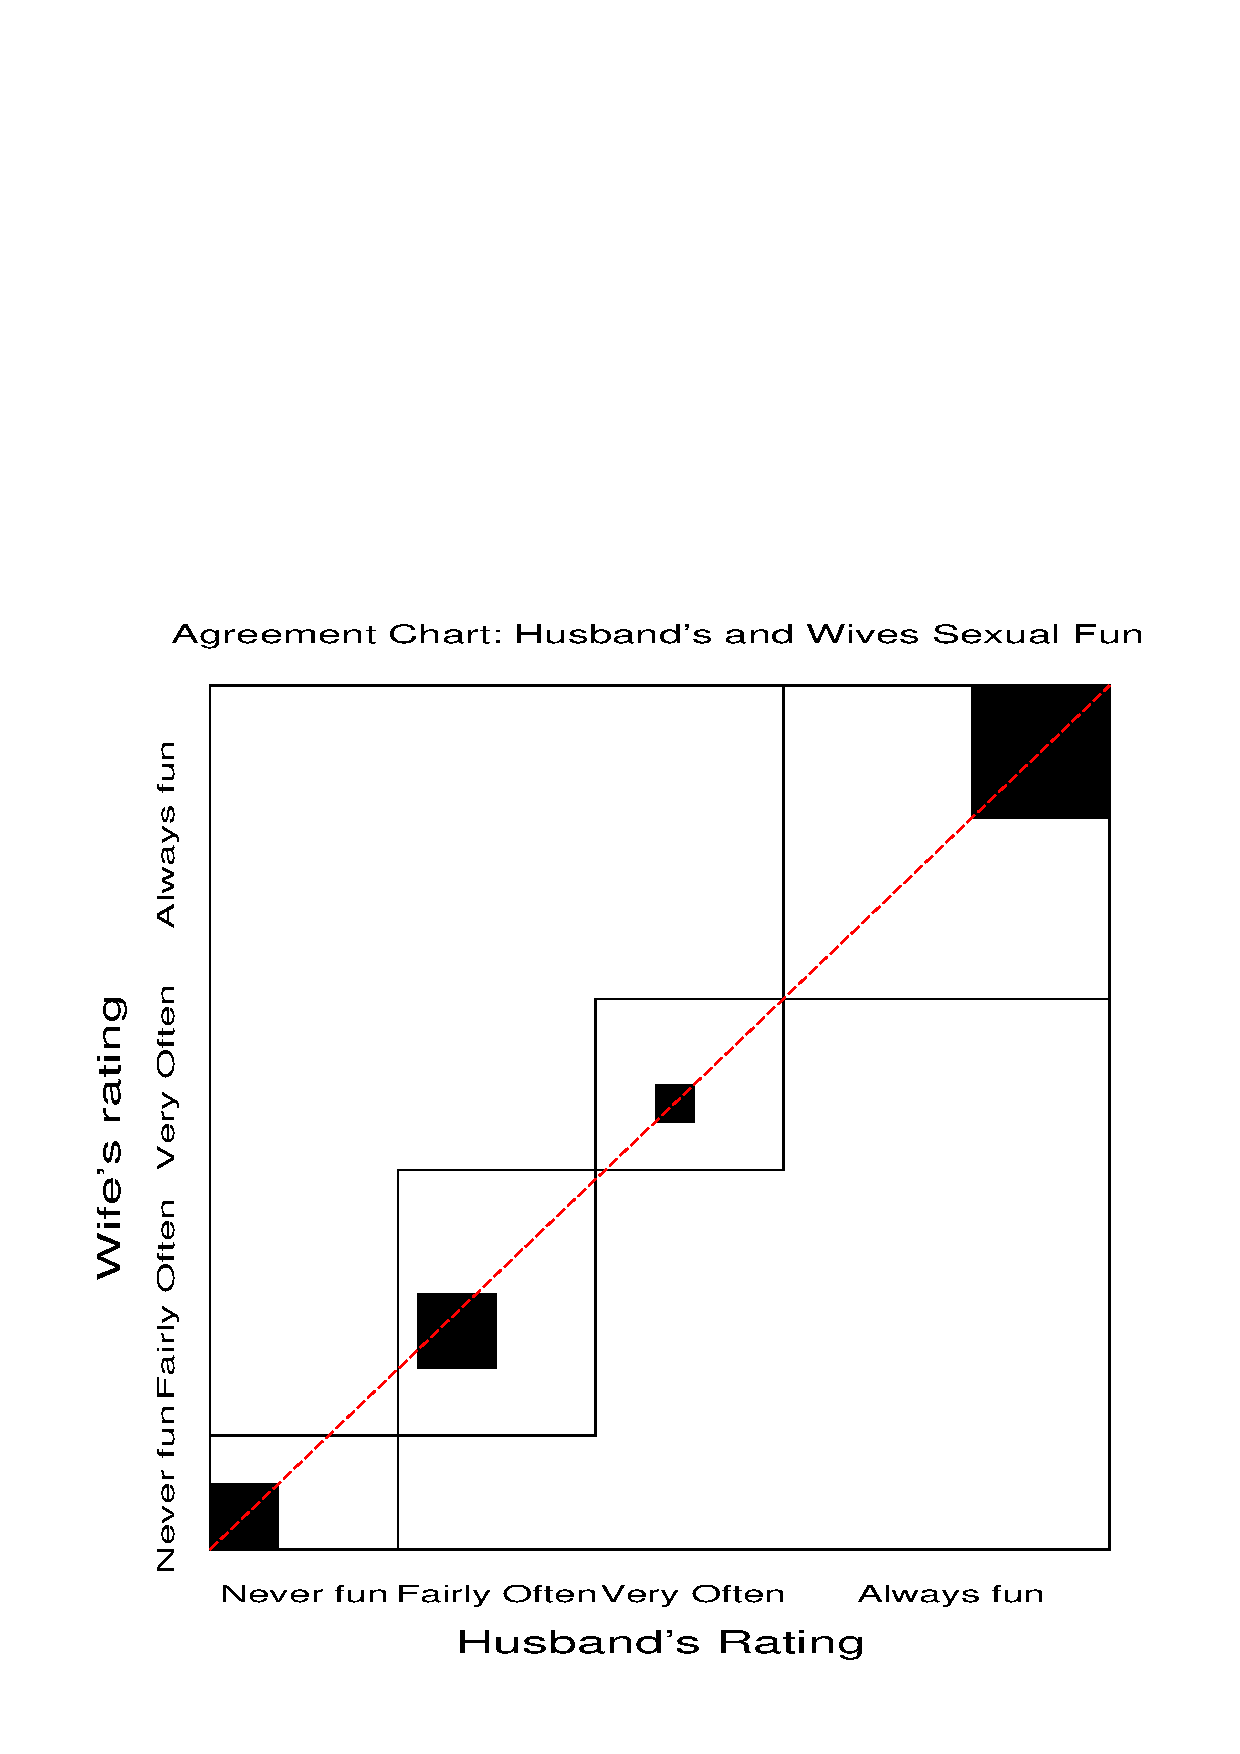
\includegraphics[width=.7\textwidth,clip,keepaspectratio]{fig/agreemt1}
 \end{center}
  
\end{frame}

\begin{frame}
  \frametitle{Weighted Agreement Chart: Partial agreement}
 Partial agreement:
include  weighted contribution from off-diagonal cells, \(b\)
steps from the main diagonal, using weights $ 1 > w_1 > w_2 > \cdots$.

  \[
 \left.
 \begin{array}{ccccc}
   &  & n_{i-b,i} &  & \\
    &  & \vdots    &  & \\
    n_{i, i-b} & \cdots & n_{i, i} & \cdots & n_{i, i+b} \\
    &  & \vdots    &  & \\
   &  & n_{i-b,i} &  &
 \end{array}
  \right.
  \qquad
 \left.
 \begin{array}{ccccc}
   &  & w_2 &  & \\
   &  & w_1 &  & \\
 w_2 & w_1 & 1 & w_1 & w_2 \\
   &  & w_1 &  & \\
   &  & w_2 &  & \\
 \end{array}
  \right.
  \]

  \begin{itemize}
	\item Add shaded rectangles, size $\sim$ sum of frequencies, \(A_{bi}\), within $b$ steps of main diagonal
	\item $\Rightarrow$ weighted measure of agreement,
  \[
  B_N^w  =
  \frac{ \mbox{weighted sum  of agreement}}
  { \mbox{area of rectangles} }  =
  1 - \frac{ \sum_i^k \,
  [ n_{i+} n_{+i} - n_{ii}^2  -
  \sum_{b=1}^q \,  w_b  A_{bi} ] }
  { \sum_i^k \,  n_{i+} \,  n_{+i} }
  \]
  \end{itemize}
\end{frame}

\begin{frame}
Husbands and wives: $B_N^w = .628$ with $w_1 = 8/9$
 \begin{center}
 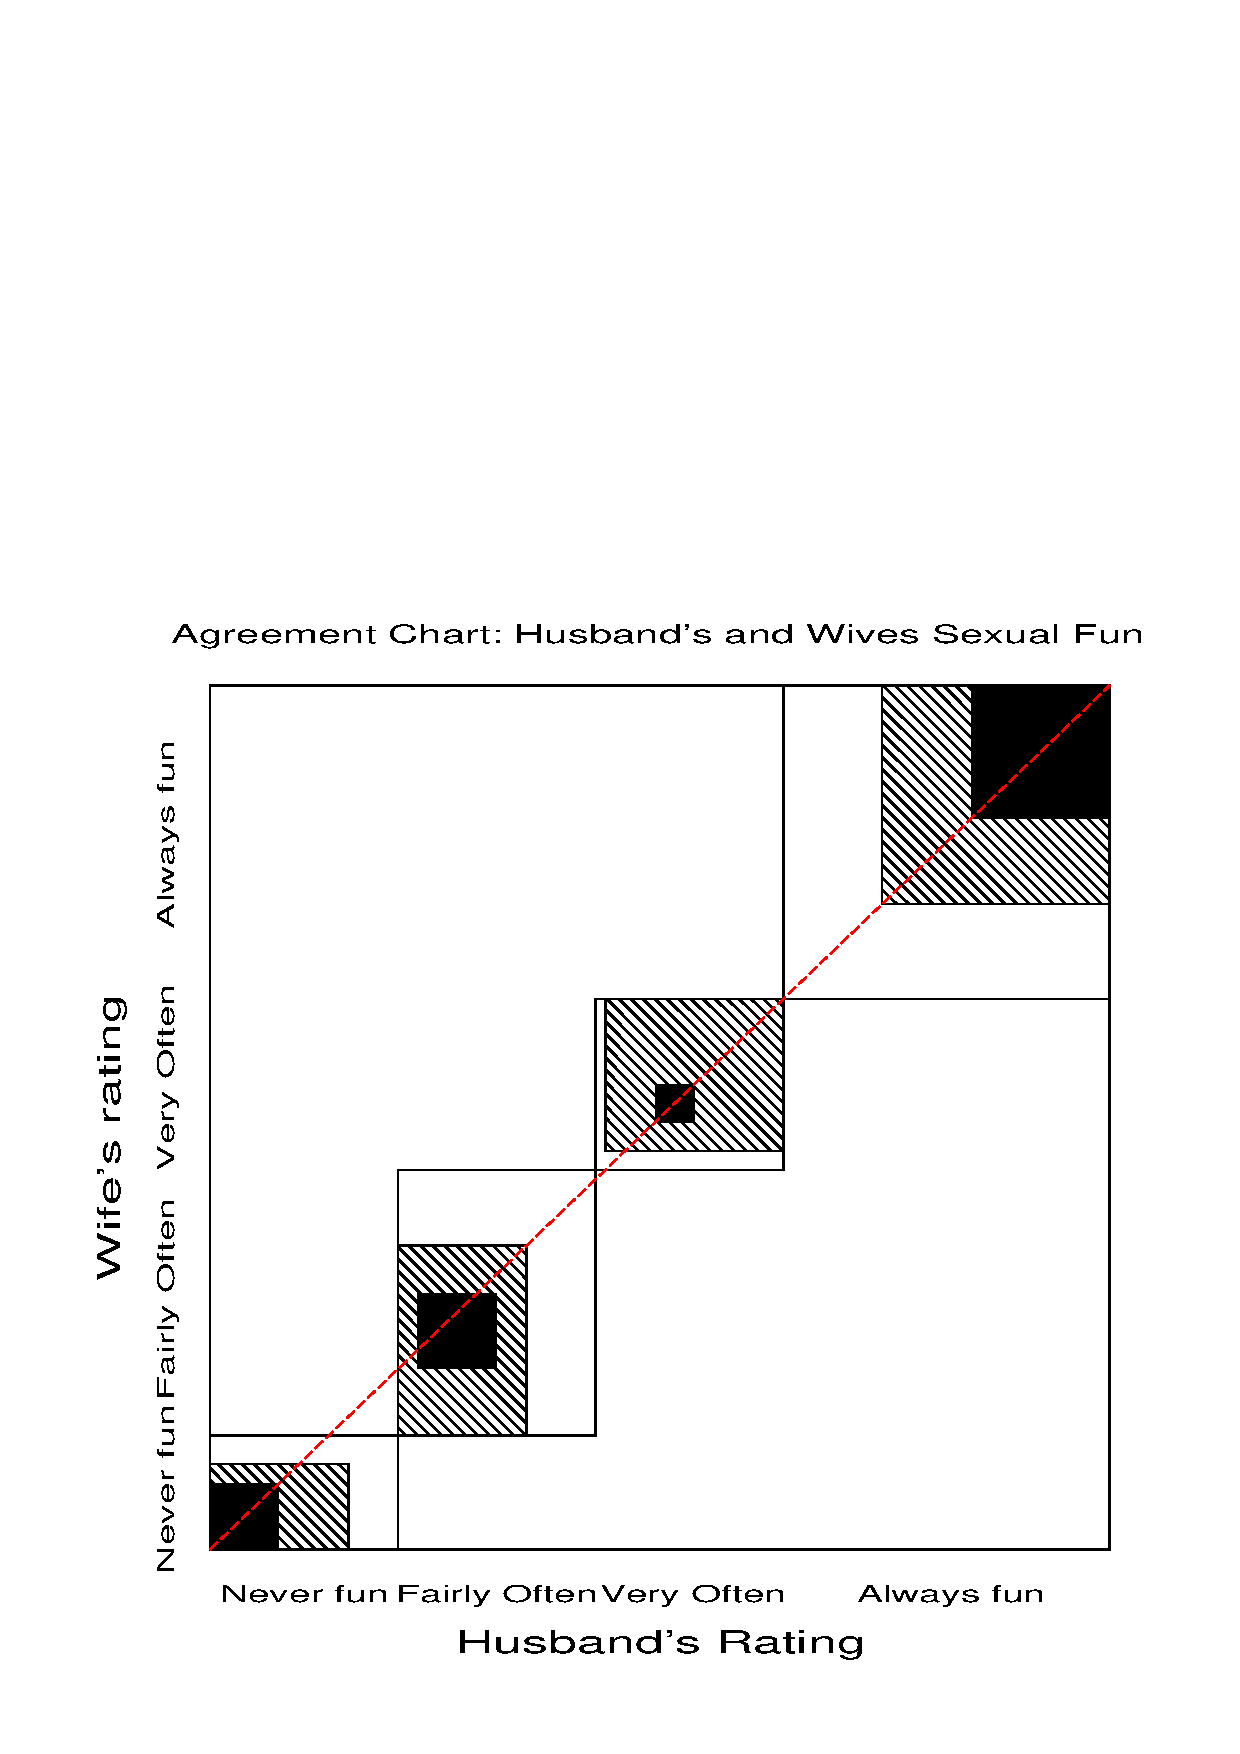
\includegraphics[width=.7\textwidth,clip,keepaspectratio]{fig/agreemt2}
 \end{center}
\end{frame}

\renewcommand{\FileName}{agree-Sex-SAS}
\begin{frame}[fragile]
\frametitle{\macrot{agreeplot}}
\begin{Input}[gobble=1,baselinestretch=0.8,fontsize=\footnotesize]
 proc format;
  value \sasemph{rating} 1='Never_fun' 2='Fairly_often' 
               3='Very_often' 4='Almost_always';
 data sexfun;
   \sasemph{format Husband Wife rating.;}
   do Husband = 1 to 4;
   do Wife    = 1 to 4;
     input count @@;
     output;
     end; end;
 datalines;
  7     7     2      3
  2     8     3      7
  1     5     4      9
  2     8     9     14
 ;

 \sascomment{*-- Convert numbers to formatted values;}
 %table(data=sexfun, var=Husband Wife, char=true, weight=count, out=table);
 %agreeplot(data=table, var=Husband Wife, title=Husband and Wife Sexual Fun);
\end{Input}
\begin{itemize*}
 \item To preserve ordering, integer values are used for Husband and Wife
 \item A SAS format is used to provide value labels
 \item The \macro{table} converts numeric $\rightarrow$ character
\end{itemize*}

\end{frame}
\renewcommand{\FileName}{agree-Sex-R}
\begin{frame}[fragile]
\frametitle{\texttt{agreementplot()} in the \pkg{vcd}}
\begin{Rin}[fontsize=\footnotesize]
> library(vcd)        # load the vcd package
> data(SexualFun)
> agreementplot(t(SexualFun), main="Agreement plot: Sex is Fun")
\end{Rin}
\begin{center}
\includegraphics[width=.45\textwidth,keepaspectratio]{fig/agree-sex}
 \end{center}
\end{frame}

\subsection{Marginal homogeneity}
\begin{frame}
  \frametitle{Marginal homogeneity and Observer bias}
  \begin{itemize*}
	\item Different raters may consistently use higher or lower response categories
	\item Test-- \boldital{marginal homogeneity}: $H_0 : n_{i+} = n_{+i}$
	\item Shows as departures of the squares from the diagonal line
 \begin{center}
 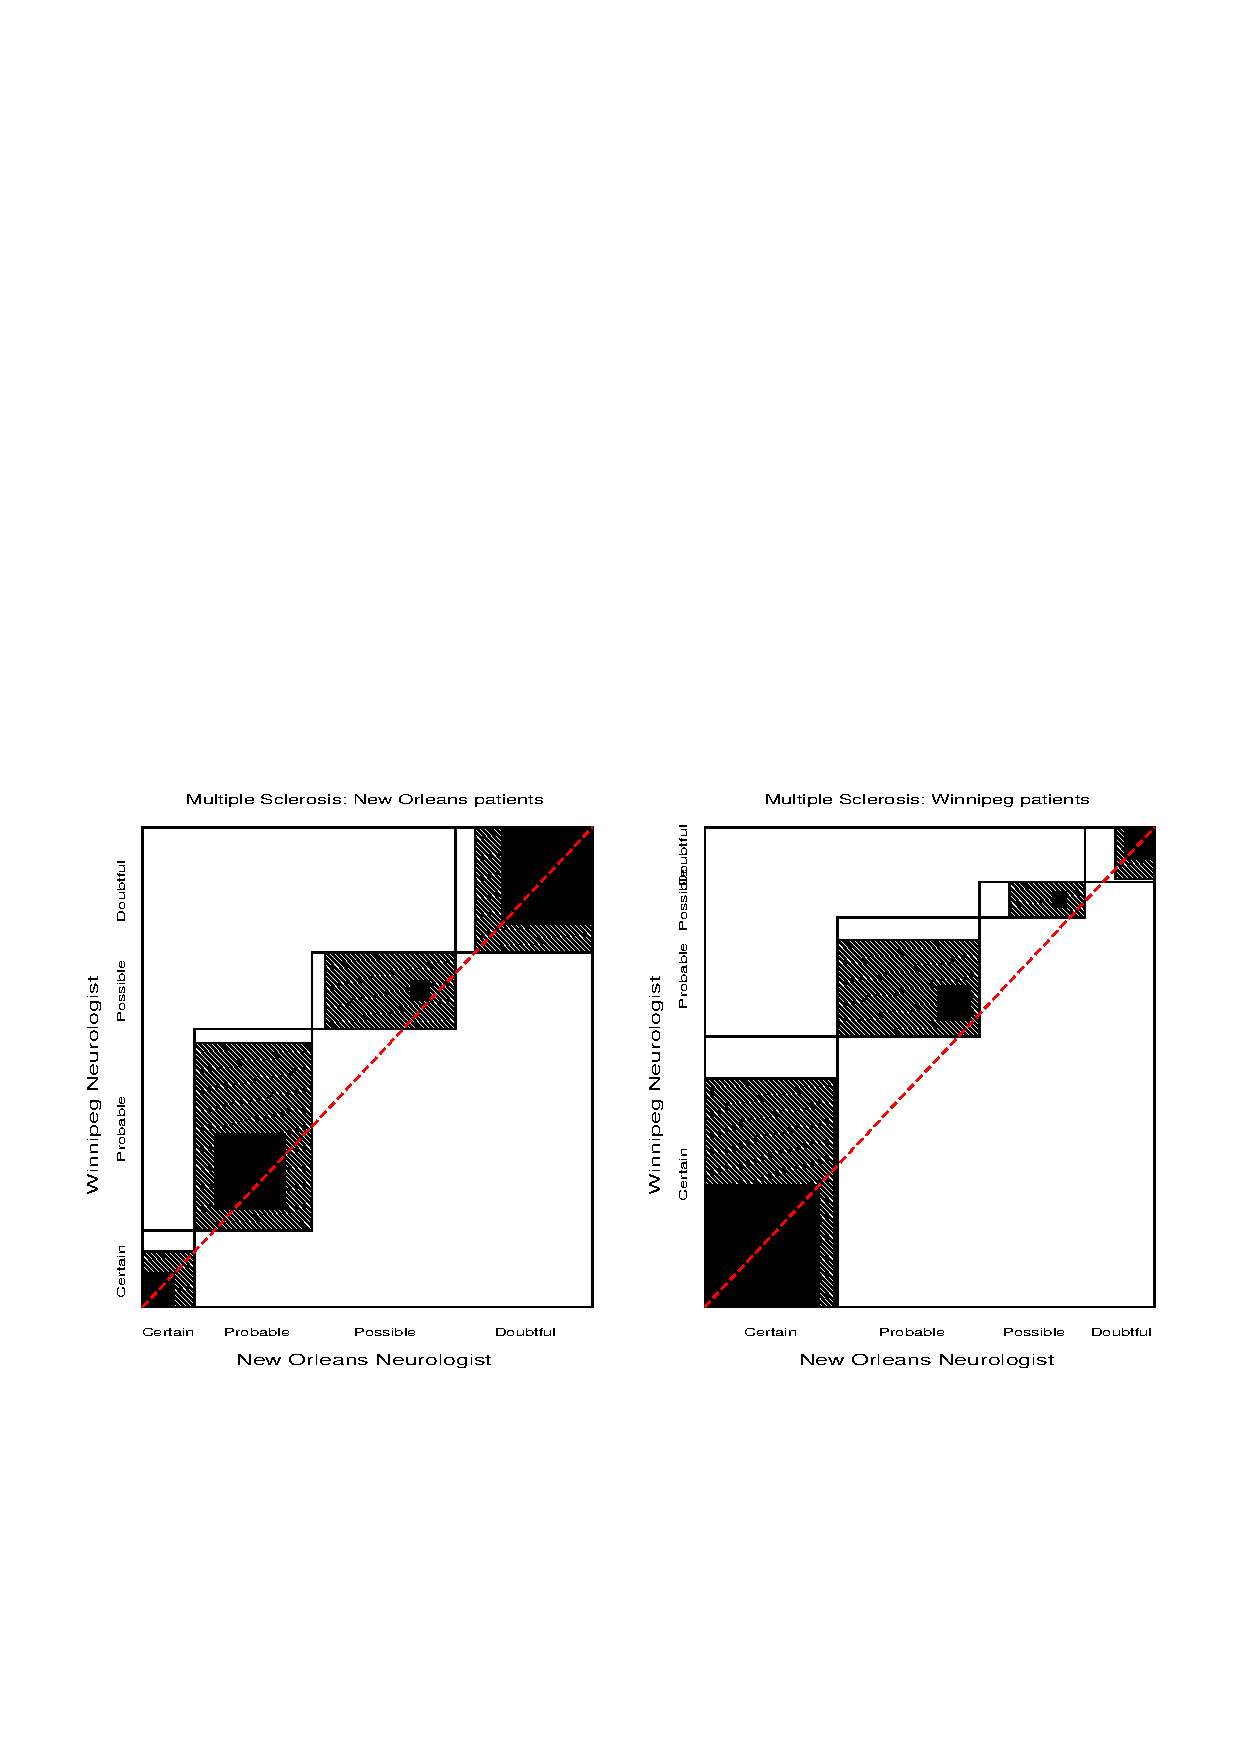
\includegraphics[width=.9\textwidth,clip]{fig/agree2}
 \end{center}
 \item Winnipeg neurologist tends to use more severe categories
  \end{itemize*}
\end{frame}

\begin{frame}[fragile]
  \frametitle{Testing marginal homogeneity}
  \begin{itemize}
	\item  Test marginal homogeneity using \PROC{CATMOD}
      \begin{itemize*}
	  \item Two tests available:
    	\begin{itemize*}
		\item Equal marginal frequencies: \texttt{RESPONSE marginals;} statement
		\item Equal mean scores: \texttt{RESPONSE means;} statement
		\end{itemize*}
      \end{itemize*}
  \end{itemize}
\begin{Input}[fontsize=\footnotesize,label=\fbox{\texttt{agreemar.sas} $\cdots$},baselinestretch=0.8]
title 'Classification of Multiple Sclerosis: Marginal Homogeneity';
proc format;
   value diagnos 1='Certain ' 2='Probable'  3='Possible'  4='Doubtful';

data ms;
 format win_diag no_diag diagnos.;
   do win_diag = 1 to 4;
   do no_diag  = 1 to 4;
      input count @@;
      if count=0 then count=1e-10;  \sascomment{/* avoid structural zeros */}
      output;
      end; end;
datalines;
   5     3     0      0
   3    11     4      0
   2    13     3      4
   1     2     4     14
;
\end{Input}
\end{frame}

\begin{frame}[fragile]
  \frametitle{Testing marginal homogeneity}
\begin{Input}[fontsize=\footnotesize,label=\fbox{$\cdots$ \texttt{agreemar.sas} $\cdots$},baselinestretch=0.8,firstnumber=20]
title2 'Testing equal marginal proportions';
proc catmod data=ms;
   weight count;
   \sasemph{response marginals;}
   model win_diag * no_diag = _response_ / oneway;
   repeated neuro 2 / _response_= neuro;
\end{Input}
Output:
\begin{Output}[gobble=5,baselinestretch=0.9]
                 Testing equal marginal proportions
                        Analysis of Variance
 
            Source         DF   Chi-Square    Pr > ChiSq
            --------------------------------------------
            Intercept       3       222.62        <.0001
            \sasemph{Neuro           3        10.54        0.0145}

            Residual        0          .           .    
\end{Output}
$\Rightarrow$ marginal proportions differ (test of \texttt{neuro})

\end{frame}

\begin{frame}[fragile]
  \frametitle{Testing marginal homogeneity}
Test of mean scores is more powerful for ordered categories:
\begin{Input}[fontsize=\footnotesize,label=\fbox{$\cdots$ \texttt{agreemar.sas}},baselinestretch=0.8,firstnumber=26]
title2 'Testing equal means';
proc catmod data=ms;
   weight count;
   \sasemph{response means;}
   model win_diag * no_diag = _response_ / oneway;
   repeated neuro 2 / _response_= neuro;
\end{Input}
Output:
\begin{Output}[gobble=5,baselinestretch=0.9]
                        Testing equal means
                        Analysis of Variance
 
            Source         DF   Chi-Square    Pr > ChiSq
            --------------------------------------------
            Intercept       1       570.61        <.0001
            \sasemph{Neuro           1         7.97        0.0048}

            Residual        0          .           .    
\end{Output}
$\Rightarrow$ test of \texttt{neuro}, on 1 df (linear) more highly significant

\end{frame}

\endinput

% slide template
\begin{frame}
  \frametitle{}
  \begin{itemize}
	\item{\large\bfseries }
      \begin{itemize*}
	  \item 
    	\begin{itemize*}
		\item 
		\item 
		\end{itemize*}
	  \item 
	  \end{itemize*}
	\item{\large\bfseries }
	\item{\large\bfseries }
  \end{itemize}
\end{frame}


\section{Trilinear plots}\label{sec:twoway-trilinear}
The \glossterm{trilinear plot}
(also called a \emph{ternary diagram} or \emph{trinomial plot})
is a specialized display for a 3-column \ctab{} or for
three variables whose relative proportions are to be displayed.
Individuals may be assigned to one of three diagnostic categories,
for example, or a chemical process may yield three constituents
in varying proportions, or we may look at the division of votes
among three parties in a parliamentary election.
This display is useful, therefore, for both frequencies
and proportions.
Trilinear plots are featured prominently in \citet{Aitchison:86},
who describes statistical models for this type of
\glossterm{compositional data}.  \citet{Upton:76,Upton:94}
uses them in detailed analyses of spatial and temporal changes in
British general elections.
\citet{Wainer:96} reviews a variety of other uses of trilinear
plots and applies them to aid in understanding the distributions
of students achievement in the
National Assessment of Educational Progress,
making some aesthetic improvements to the traditional form of these
plots along the way.

A trilinear plot displays each observation as a point inside
an equilateral triangle whose coordinate corresponds to the
relative proportions in each column.
The three vertices represent the three extremes when 100\%
occurs in one of the three columns; a point in the exact
center corresponds to equal proportions of $\frac13$ in
all three columns.  For instance, \figref{fig:tripdemo2}
shows how three points whose compositions of three variables,
A, B, and C are shown as annotations.
Note that each apex corresponds to 100\% of the labeled
variable, and the percentage of this variable decrease
linearly along a line to the midpoint of the opposite
baseline.
The grid lines in the figure show the percentage value along
each axis.

\begin{figure}[htb]
  \centering
  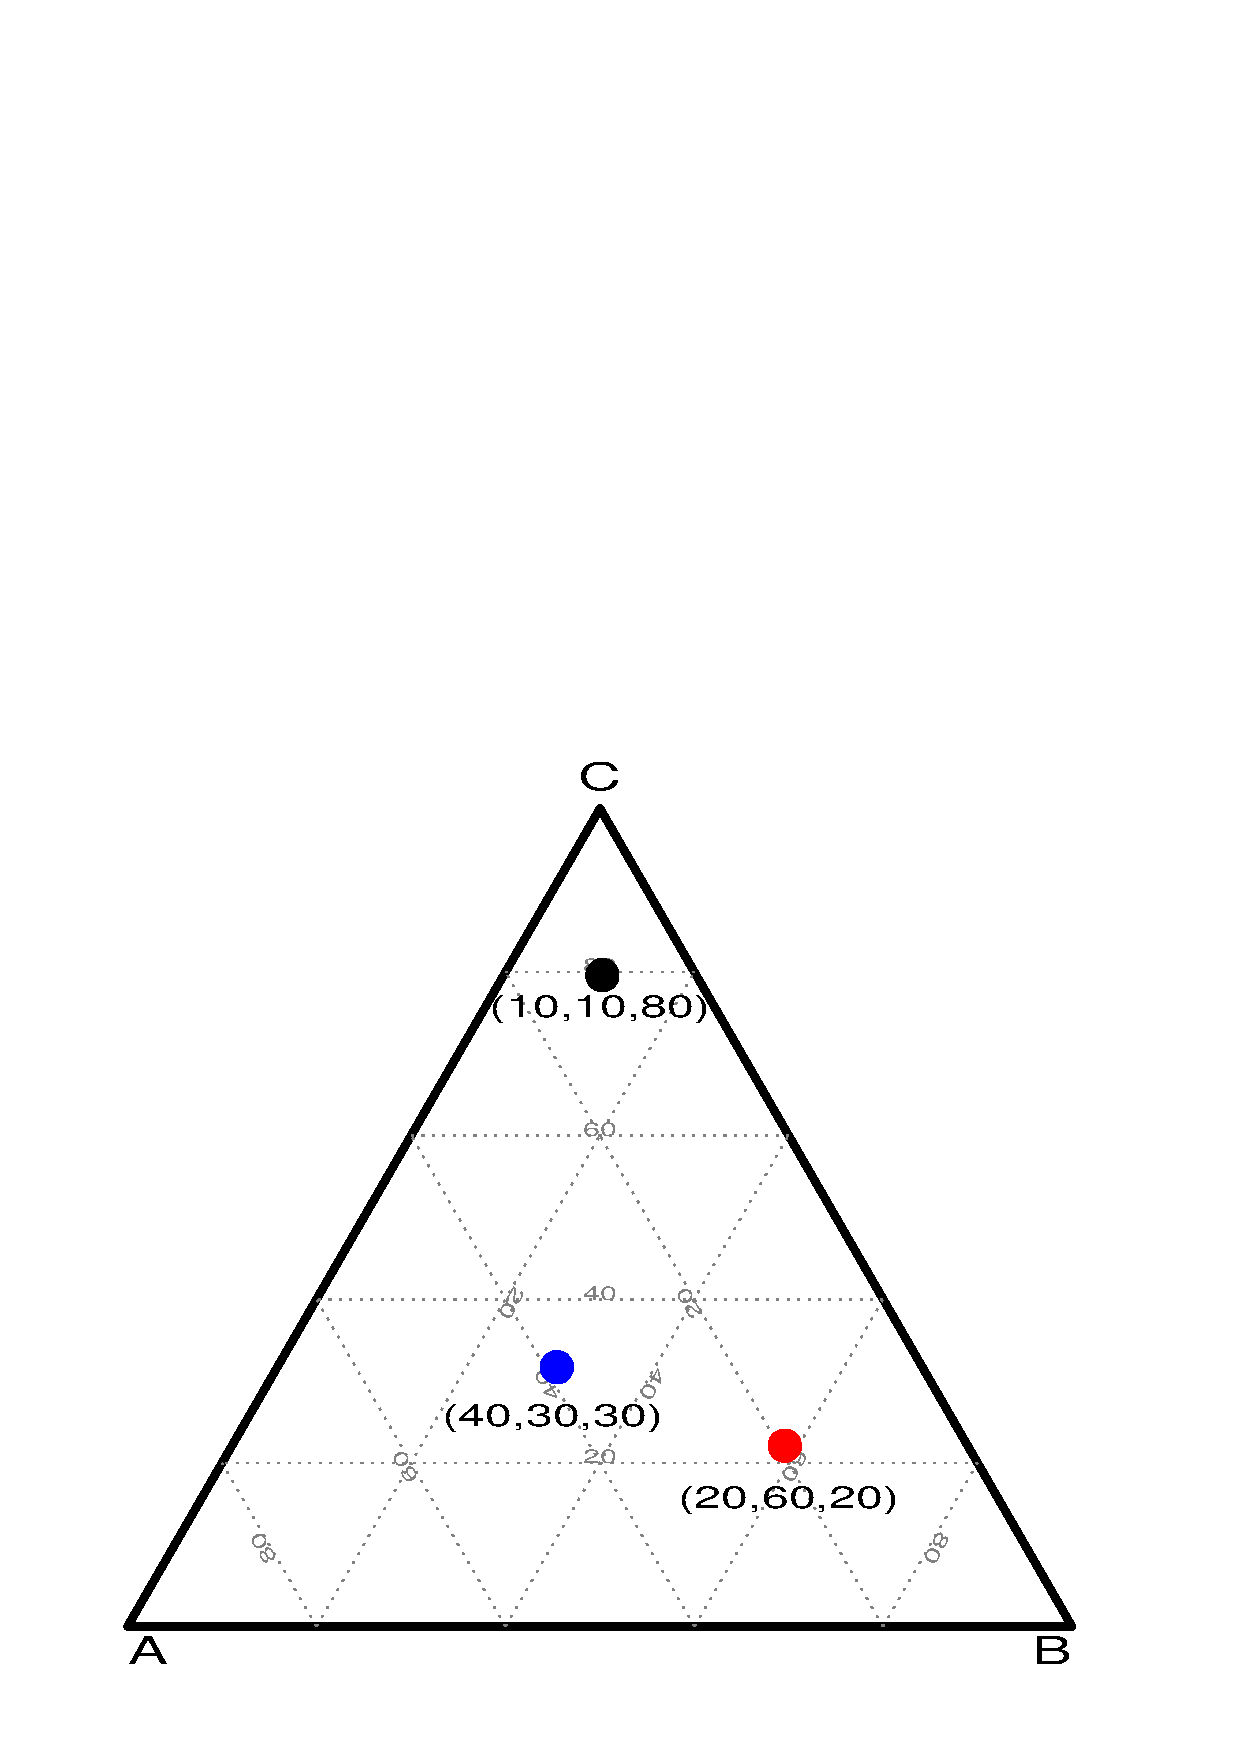
\includegraphics[scale=.6]{ch3/fig/tripdemo2}
  \caption[A trilinear plot]{An illustrative trilinear plot}\label{fig:tripdemo2}
\end{figure}

The construction of trilinear plots is described in detail
by \citet{FedenczukBercov:91}.
Briefly, let $P(a, b, c)$ represent the three components  normalized so
that $a + b + c = 1.0$.
If the apex corresponding to Point A in \figref{fig:tripdemo2}
is given $(x, y)$ coordinates of $(x_A, y_A) = (0, 0)$,
and those at apex B are $(x_B, y_B) = (100, 0)$,
then the coordinates of apex C are $(x_C, y_C) = (50, 50\sqrt{3})$.
The coordinates $(x_P, y_P)$  of $P$ are then calculated as
\begin{eqnarray*}
y_P & = & c \: y_C \\
x_P & = & y_P \left( \frac{y_C - y_B}{x_C - x_B} \right)
+ \frac{\sqrt{3}}{2} y_C (1 - a) \\
\end{eqnarray*}

The figures shown here are produced using the \macro{TRIPLOT},
which is listed in \macref{mac:triplot}.

\begin{Example}[arthrit5]{Arthritis treatment}
%\example{Arthritis treatment}
In the Arthritis treatment data, our interest is focused on the
relative numbers of individuals in the three outcome categories
for the four groups defined by the combinations of Treatment
and Sex.

\figref{fig:arthtri} shows clearly that both groups given the
active treatment result in greater proportions of successful
outcomes (some or marked improvement) than do the placebo
groups.
In addition, regardless of treatment, females show greater
proportions of successful outcomes than do males.

\begin{figure}[htb]
  \centering
  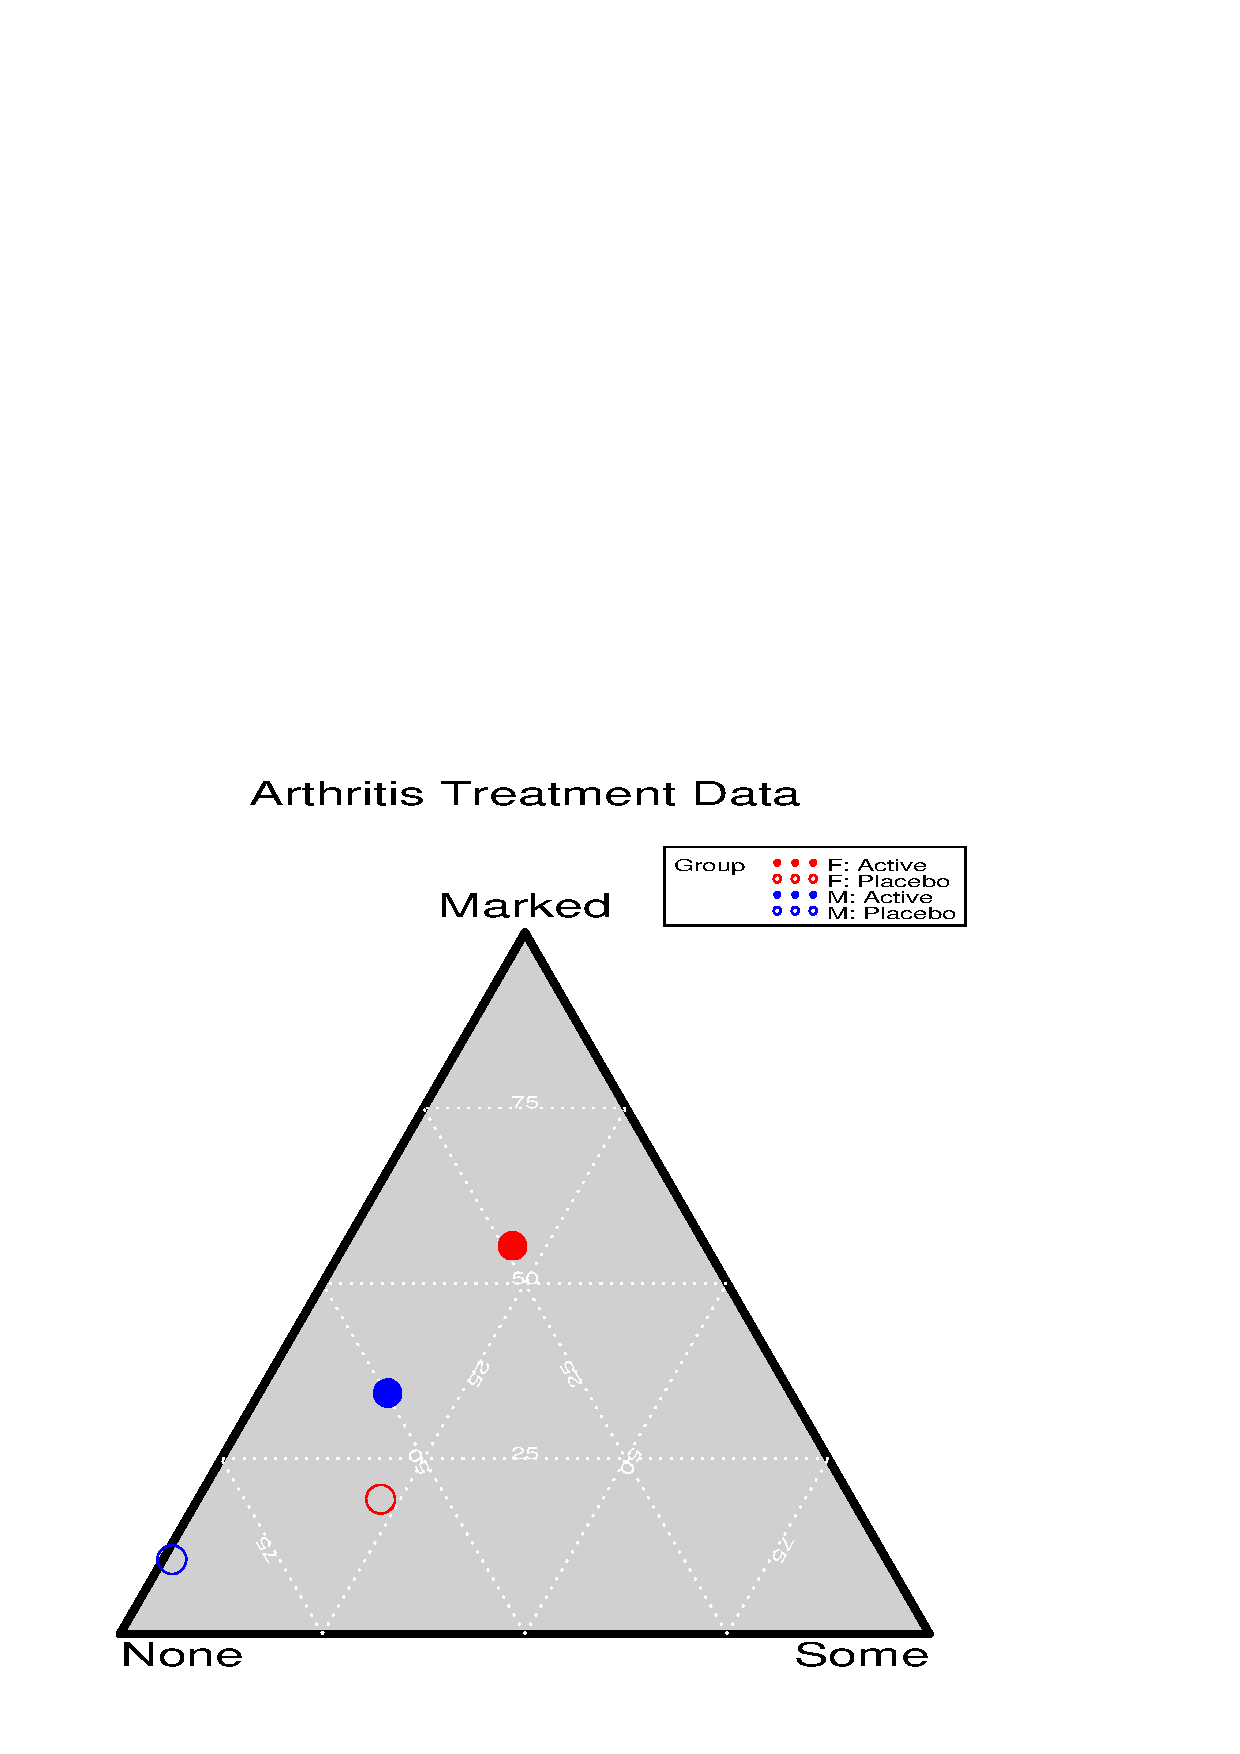
\includegraphics[scale=.6]{ch3/fig/arthtri}
  \caption[Trilinear plot for Arthritis treatment data]{Trilinear plot for Arthritis treatment data}\label{fig:arthtri}
\end{figure}

\figref{fig:arthtri} is produced using the \macro{TRIPLOT}
as follows.  For convenience in identifying the treatment-sex combinations,
these two variables are combined into a single \texttt{GROUP} variable,
used as the value of the \texttt{CLASS=} parameter in the macro call.
%% input: /users/faculty/friendly/sasuser/catdata/arthtri.sas
%% last modified: 14-Jan-98 14:02
\begin{listing}
title 'Arthritis Treatment Data';
data arth;
   input sex $ treat $ @;
   input none some marked;
   length group $10;
   sex = substr(sex,1,1);
   group = trim(sex) || ': ' || treat;
   label group='Group';
datalines;
Female  Active    6  5  16
Female  Placebo  19  7   6
Male    Active    7  2   5
Male    Placebo  10  0   1
;
%triplot(data=arth,
   var=None Some Marked, class=group,
   symht=4, 
   symbols=dot circle dot circle,
   colors=red red blue blue, 
   backclr=grayd0, backpat=solid,
   gridclr=white, gridby=25);
\end{listing}

\end{Example}

\begin{Example}[baseball]{Baseball fielding}
The \emph{Baseball \Dset} from \SSSGref{A2.3}
includes data on the salaries and batting and fielding performance of 322 major league in the 1986 baseball season.
Fielding performance includes the numbers of Errors,
Putouts and Assists made by each player.
(Putouts occur when a fielder causes an opposing player to be tagged or forced out;
assists are credited to other fielders involved in making that
putout.)

\figref{fig:basetri} shows a triplot for this data.
Because of the large number of observations in the \Dset,
the mean number of putouts, assists and errors was calculated for each team
and for each position, giving a reduced \Dset\ of 169 observations.%
\footnote{Putouts and assists also occur far more often than errors,
so the values of each variable were also first scaled to a common range.}
These observations are graphed in \figref{fig:basetri} coding the
player's position by the plotting symbol.

\begin{figure}[htb]
  \centering
  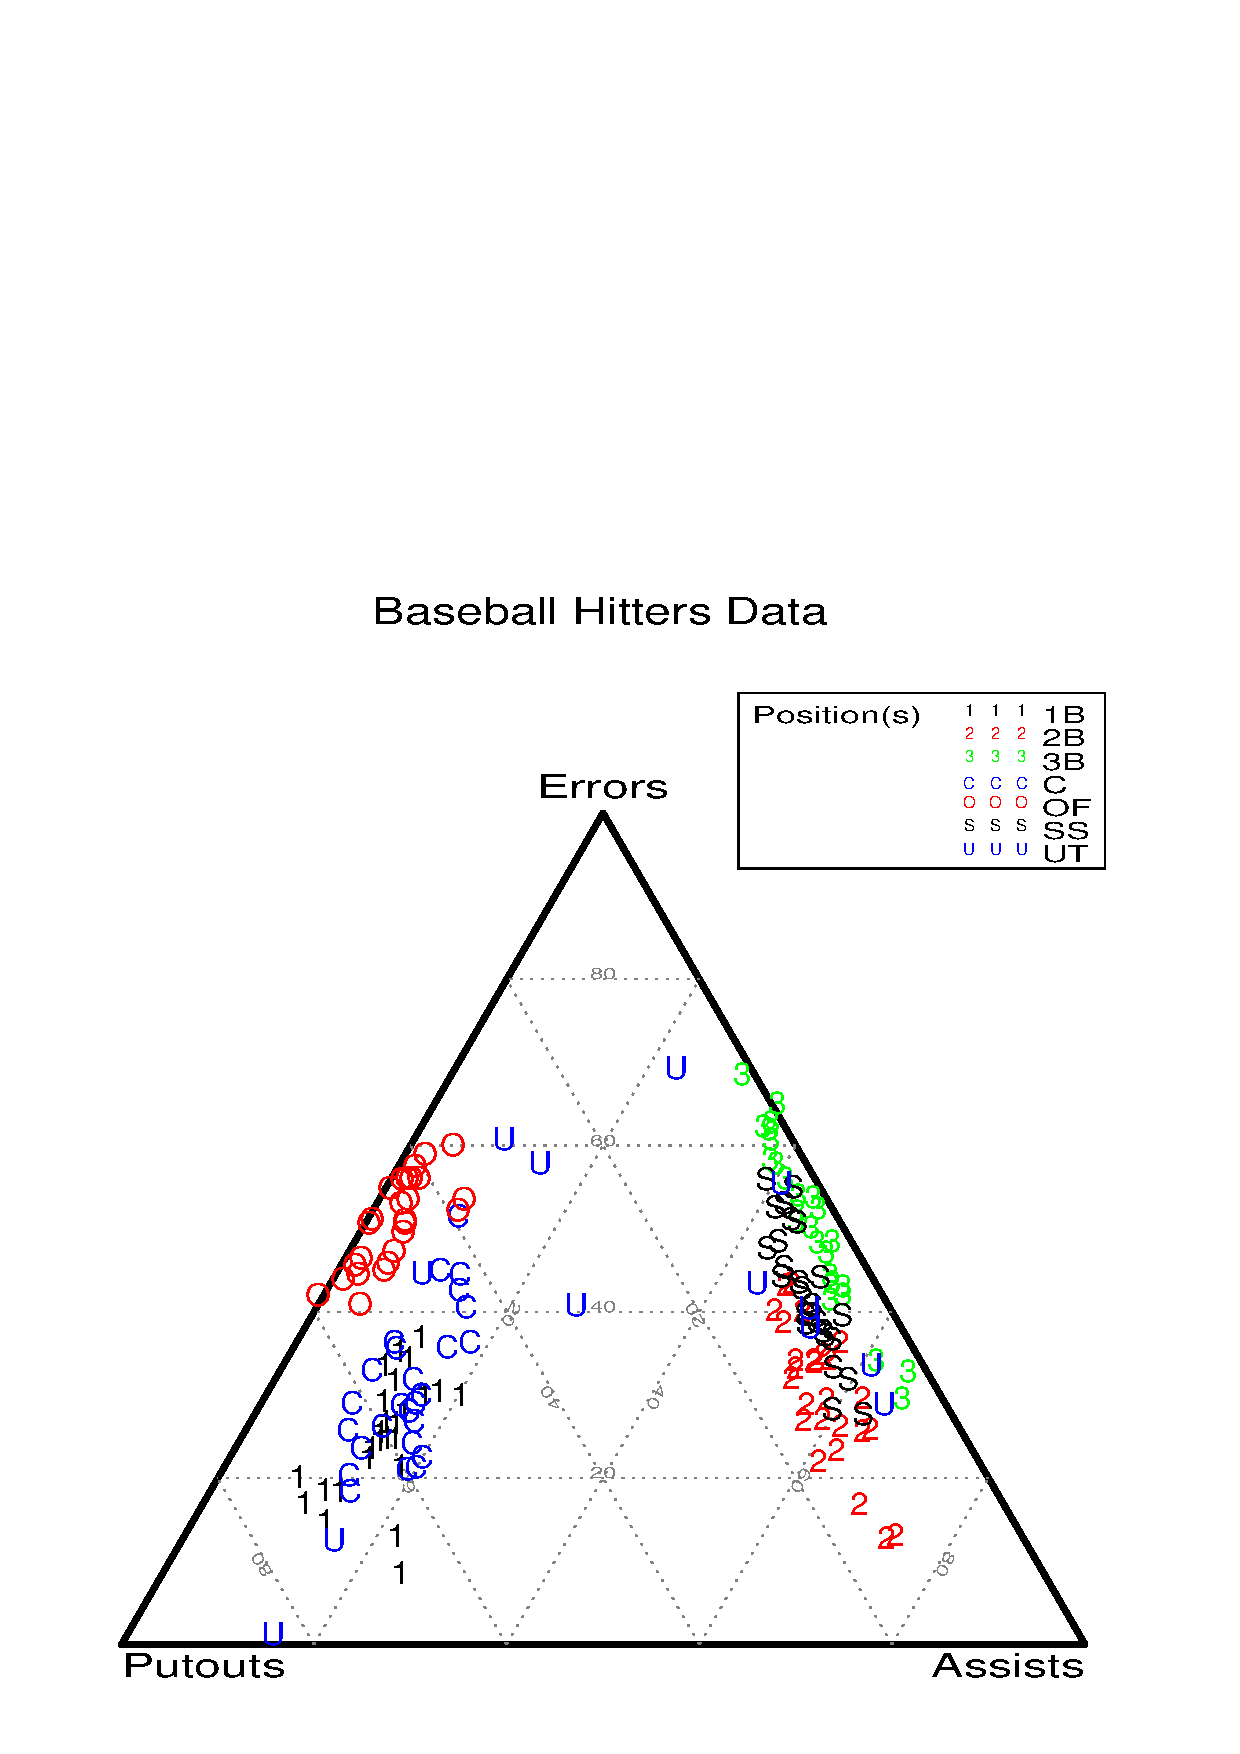
\includegraphics[scale=.6]{ch3/fig/basetri}
  \caption[Trilinear plot for baseball data]{Trilinear plot for baseball fielding data}\label{fig:basetri}
\end{figure}

It may be seen that two main types of
players may be distinguished by their relative proportions of
putouts and assists: Outfielders, catchers and first basemen
contribute to defense primarily in making putouts; other infielders
primarily make assists.  The utility players (UT) play in a variety
of positions and are scattered throughout the plot.
Beyond this main observation, you can also see that outfielders and
third basemen tend to make more errors than players in other positions.
\end{Example}

\begin{Example}[lifeboat1]{Lifeboats on the \emph{Titanic}}
We examine the question of who survived and why in the sinking of the \emph{RMS Titanic} in \secref{sec:mosaic-threeway} (\exref{ex:titanic}),
where we analyze a four-way table of the 2201 people on board (1316 passengers and 885 crew),
classified by Class, Sex, Age, and Survival.
A different \Dset\ which sheds some light on the same issues is
appropriate here.

After the disaster, the British Board of Trade launched several
inquiries, the most comprehensive of which resulted in the
\emph{Report on the Loss of the ``Titanic'' (S.S.)}
by Lord Mersey
\citep{Mersey:1912}.
Section 4 of this document contains a detailed account of the saving
and rescue of the passengers and crew who survived.
The \emph{Titanic} was outfitted with 20 boats, half on each of the
port and starboard sides,
 of which 14 were large
lifeboats with a capacity of 65, two were emergency boats designed for
40 persons, and the remaining four were collapsible boats capable of holding
47, a total capacity of 1178 (considered adequate at that time).
Two of the collapsible boats, lashed to the roof of the officers
quarters, were ineffectively launched and utilized as rafts after the ship sunk.
The report lists the time of launch and composition of the remaining 18 boats according to male passengers, women and children, and ``men of crew'',
as reported by witnesses.
The \Dset\ \texttt{lifeboat} (see \datref{dat:lifeboat})
contains the data listed on p. 38 of that report.%
\footnote{The ``data'' lists a total of 854 in 18 boats, although only
712 were in fact saved.  Mersey notes ``it is obvious that these figures
are quite unreliable''.  Allowing for 60 people rescued from the water,
only 652 could have left in the boats \citep[p. 39]{Mersey:1912}.
We present an alternative \Dset, \pname{LIFEBOA2}, in \datref{dat:lifeboat},
based on more conservative and historically accurate informatio.}

Of interest here is the composition of the boats by these three categories
and according to the launching of the boats from the port or starboard
side, which can be shown in a trilinear display
using the following statements.
The parameter \pname{idsubset = men>.1} is used to label only boats
in which the proportion of male passengers exceeded 10\%.
(The values of variables have been scaled to sum to 1.0 for each observation
at the time the \mparm{idsubset}{TRIPLOT} is used.)
The \pname{labloc=0} parameter is used to label the axes at the value
corresponding to 0\%
rather than at the vertex (\pname{labloc=100}) as in the earlier plots.

\begin{listing}
legend1  position=(top right inside) across=1
   offset=(0,-25pct) mode=share frame;
%triplot(data=lifeboat,
   var=Crew Men Women,
   id=boat, class=side,
   legend=legend1, labloc=0,
   idht=1.7, symht=1.7,
   idsubset=men>.1,
   symbols= circle dot, colors=red blue);
\end{listing}
\begin{figure}[htb]
  \centering
  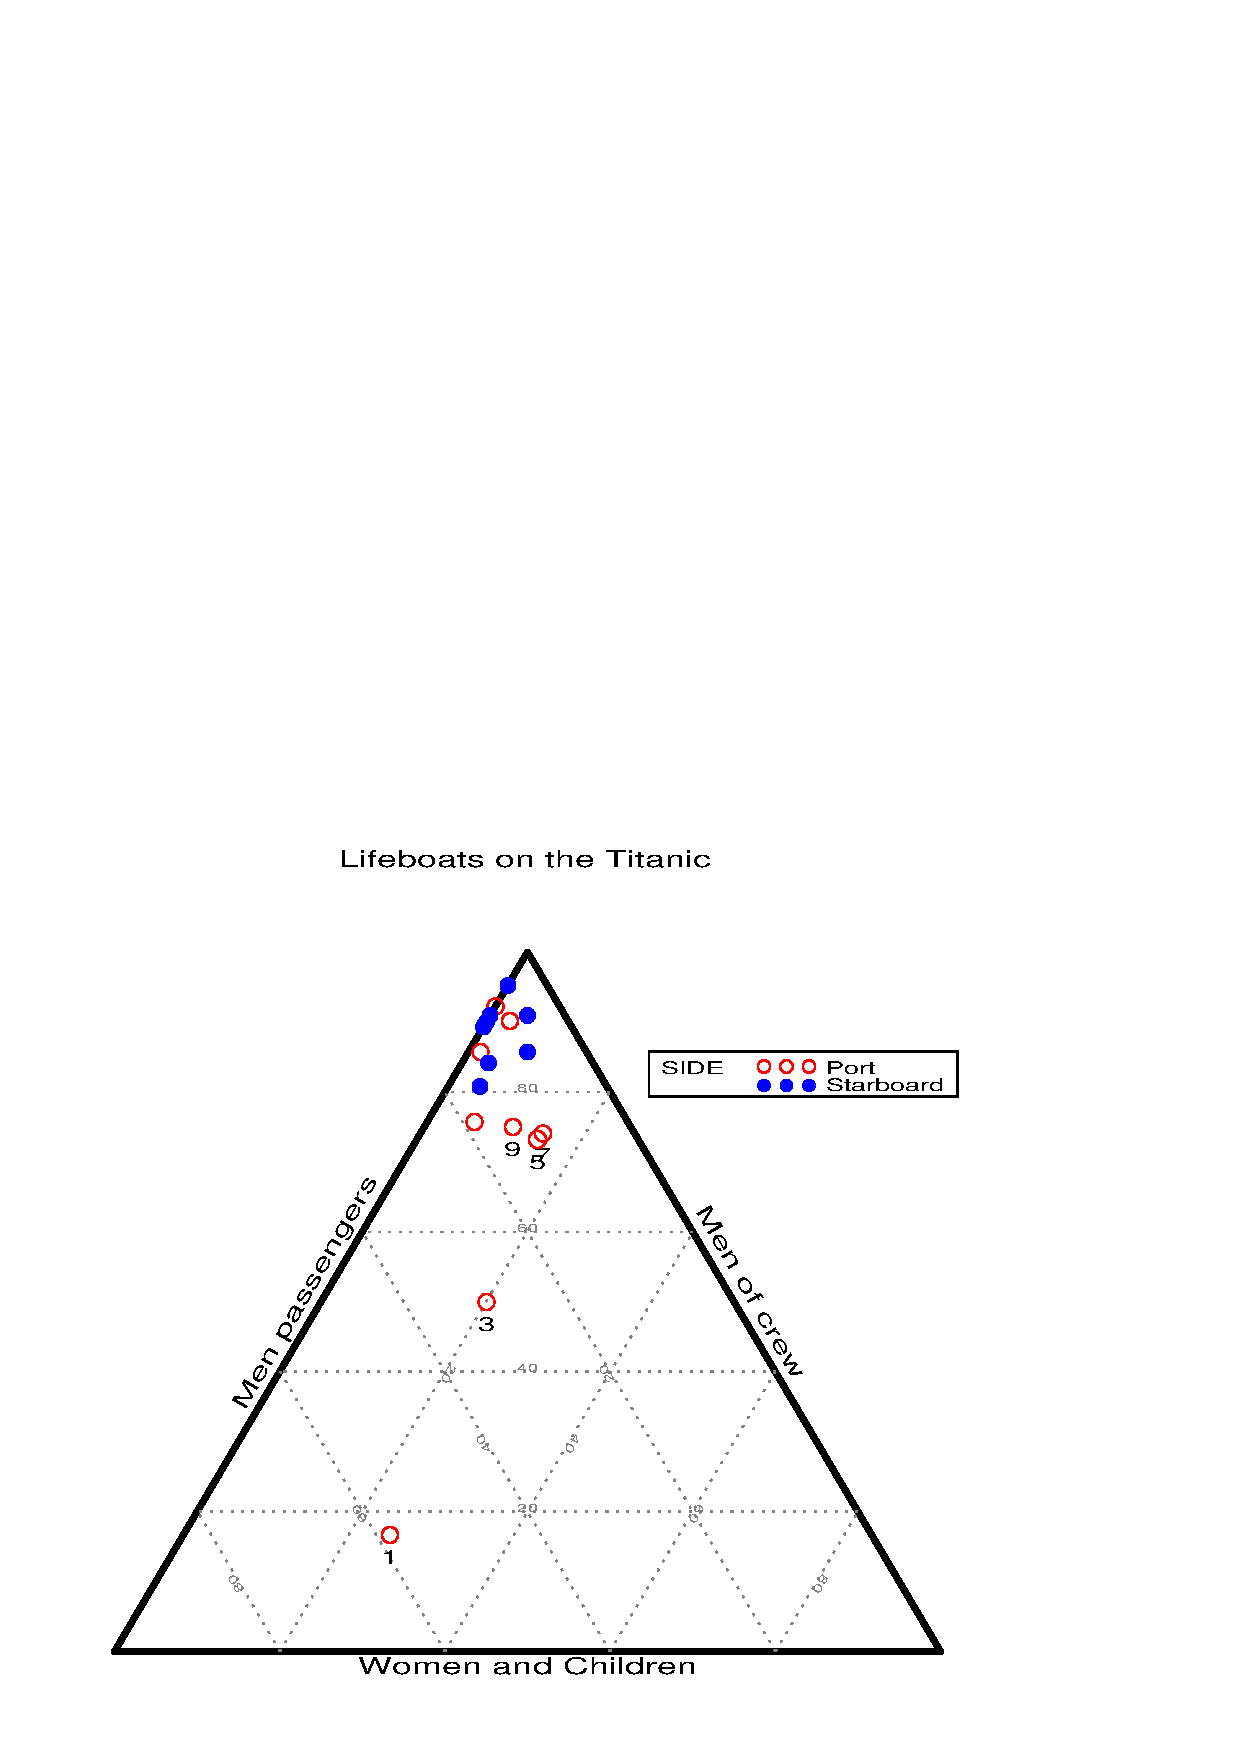
\includegraphics[scale=.6]{ch3/fig/lifeboat1}
  \caption[Lifeboats on the \emph{Titanic}]{Lifeboats on the \emph{Titanic},
  showing the composition of each boat.  Boats with more than 10\% male
  passengers are labeled.}%
  \label{fig:lifeboat1}
\end{figure}

The result, shown in \figref{fig:lifeboat1}, makes it immediately apparent
that many of the boats launched from the port side differ substantially
from the remaining boats, whose passengers were almost entirely women
and children.  Boat 1 had only 20\% (2 out of 10) women and children, while the percentage for boat 3 was only 50\% (25 out of 50).


The triplot scales the numbers for each observation to sum to 1.0,
so differences in the total number of people on each boat
cannot be seen in \figref{fig:lifeboat1}.
The total number reported loaded is plotted against launch time in \figref{fig:lifeboat2},
with a separate regression line fit to the data for the port and starboard
sides.
It seems clear that the rescue effort began in panic on the port side,
with relatively small numbers loaded, and (from \figref{fig:lifeboat1}),
small proportions of women and children.
But the loading regime improved steadily over time.
The procedures began more efficiently on the starboard side
and the numbers loaded increased only slightly, though still
with large variability from boat to boat.
\begin{figure}[htb]
  \centering
  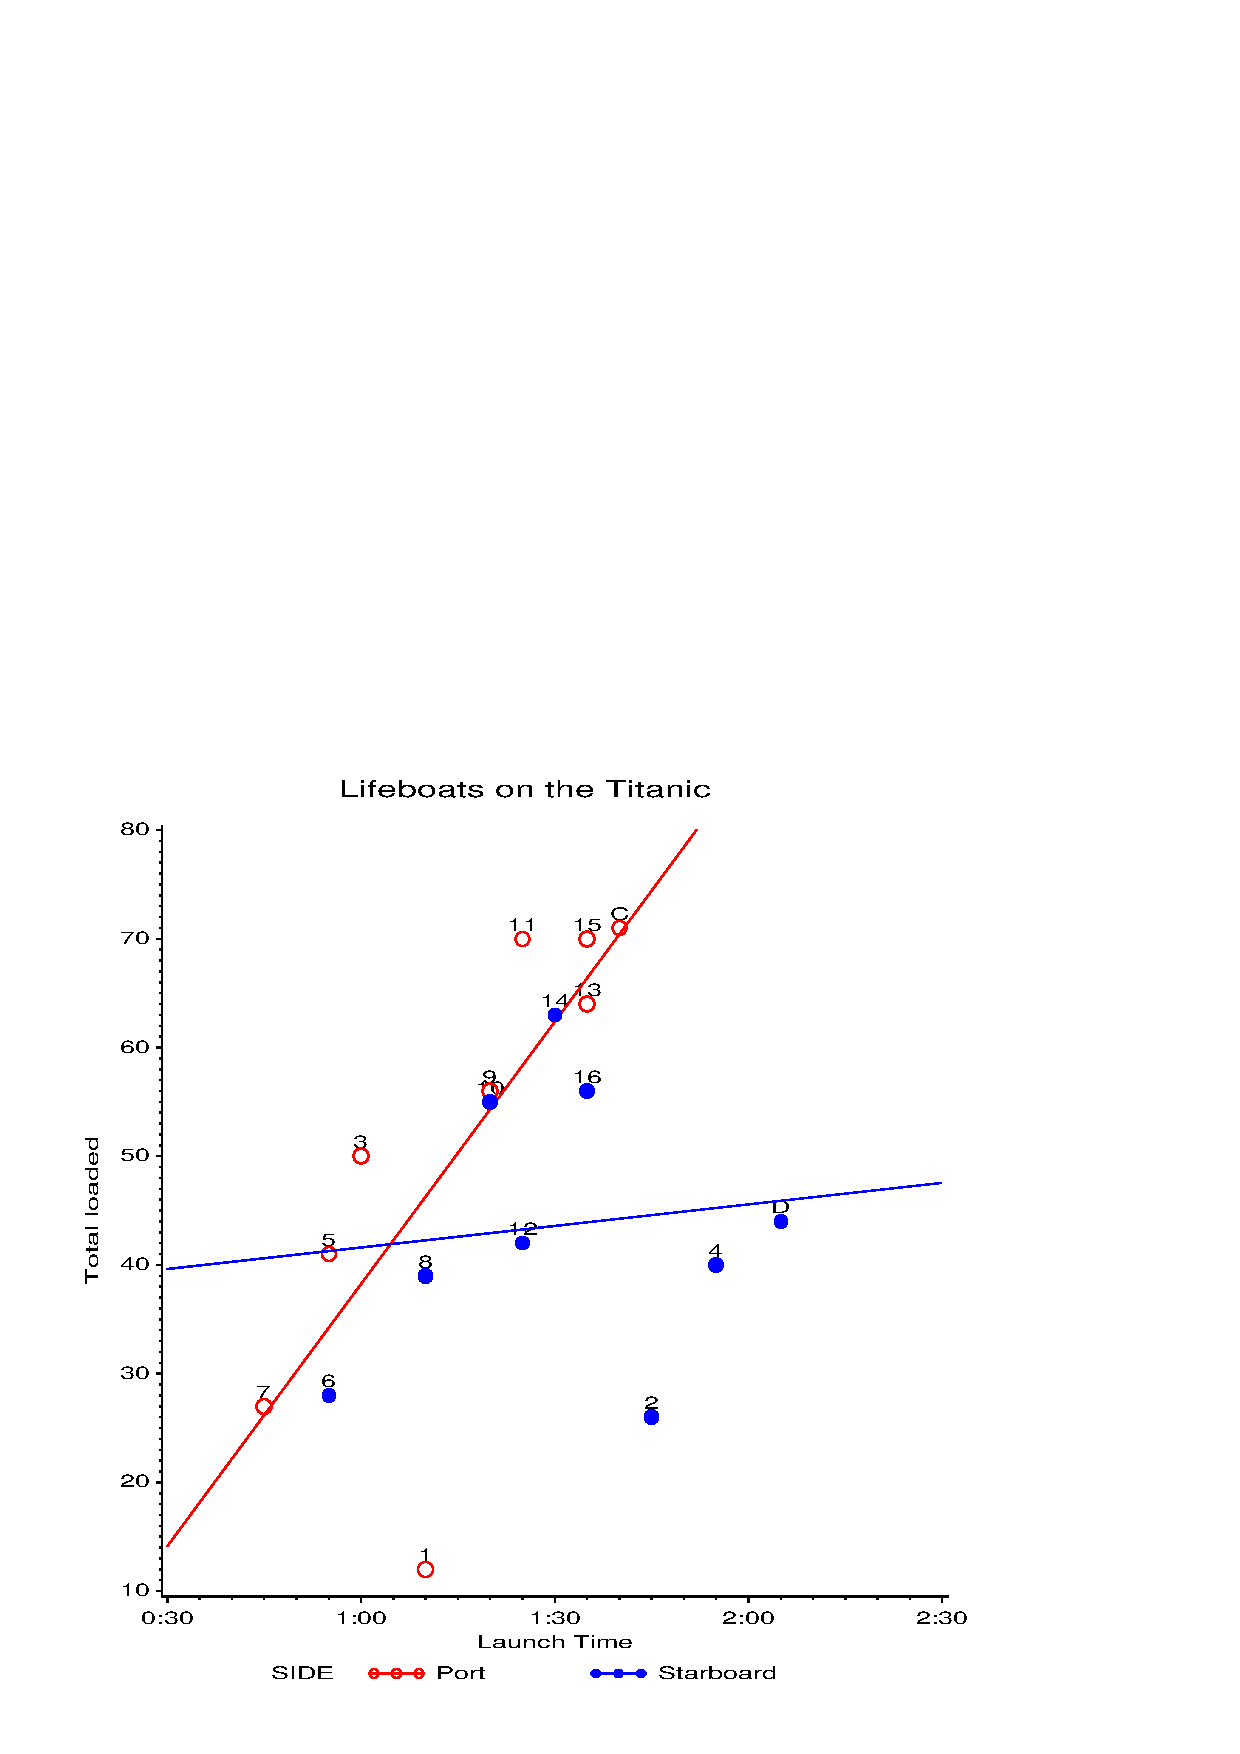
\includegraphics[scale=.6]{ch3/fig/lifeboat2}
  \caption[Lifeboats on the \emph{Titanic}]{Lifeboats on the \emph{Titanic},
  showing the numbers loaded on each boat.
  Regression lines for each side indicate a difference in regimes for
  the port and starboard sides.}%
  \label{fig:lifeboat2}
\end{figure}
\end{Example}



%\section{Chapter summary}
\begin{itemize}
\item Correspondence analysis is an exploratory technique, designed to
show the row and column categories in a two- (or three-) dimensional
space.  These graphical displays, and various extensions, provide
ways to interpret the patterns of association and visually explore 
the adequacy of certain \loglin models.

\item The scores assigned to the categories of each variable are optimal
in several equivalent ways.
Among other properties,
they maximize the (canonical) correlations between the quantified
variables (weighted by cell frequencies), and make the regressions
of each variable on the other most nearly linear, for each CA dimension.

\item Multi-way tables may be analyzed in several ways.
In the ``stacking'' approach, two or more variables may be combined
interactively in the rows and/or columns of an \nway table.
Simple CA of the restructured table reveals associations between
the row and column categories of the restructured table,
but hides associations between the variables combined interactively.
Each way of stacking corresponds to a particular \loglin model
for the full table.

\item Multiple \ca is a generalization of CA to two or more variables
based on representing the data as an indicator matrix, or the Burt matrix.
The usual MCA provides an analysis of the joint, bivariate relations
between all pairs of variables.

% \item An extended form of MCA provides a means to display higher-order
% associations among multiple categorical variables.
% For $2^Q$ tables composed of $Q$ binary variables, this analysis yields
% simple geometric relations that may be interpreted in terms of odds ratios.
% \TODO{Delete this if \secref{sec:ca-mcainter} is not included.}

\item The biplot is a related technique for visualizing the elements of
a data array by points or vectors in a joint display of their row and
column categories. A standard CA biplot represents the contributions to
lack of independence as the projection of the points for rows
(or columns) on vectors for the other categories.

\item Another application of the biplot to \ctab data is described, based on analysis
of log frequency.
This analysis also serves to diagnose patterns of independence and
partial independence in two-way and larger tables.
\end{itemize}

%\section{Further reading}
